%\documentclass[prb, twocolumn, 12pt]{revtex4}
%nofootinbib
\documentclass[pra,twocolumn,groupedaddress,10pt]{revtex4}

\usepackage[papersize={8.5in,11in}]{geometry} % set page size in a standard way
\usepackage{amsmath}    % need for subequations
\usepackage{amsthm}     % need for theorems and definitions
\usepackage{amssymb}     % need for symbols like \varnothing
\usepackage{graphicx}   % need for figures
\usepackage{verbatim}   % useful for program listings
\usepackage{color}      % use if color is used in text
\usepackage{subfigure}  % use for side-by-side figures
\usepackage{hyperref}   % use for hypertext links, including those to external documents and URLs
\usepackage{tikz}
%\usepackage{tikz,fullpage}
\usetikzlibrary{arrows,%
                petri,%
                topaths}%
\usepackage{tkz-berge}
\usepackage{tikz-cd}
\usepackage{mathrsfs}
\usepackage{hyperref}
\usepackage{thmtools}
\usepgflibrary{shapes}
\usepackage{url}
\usepackage[stretch=10]{microtype}
\usepackage{enumitem}

%\usepackage[position=top]{subfig}


% don't need the following. simply use defaults
\setlength{\baselineskip}{16.0pt}    % 16 pt usual spacing between lines

% below float fixing from mintaka.sdsu.edu/GF/bibliog/latex/floats.html
% Alter some LaTeX defaults for better treatment of figures:
    % See p.105 of "TeX Unbound" for suggested values.
    % See pp. 199-200 of Lamport's "LaTeX" book for details.
    %   General parameters, for ALL pages:
    \renewcommand{\topfraction}{0.9}	% max fraction of floats at top
    \renewcommand{\bottomfraction}{0.8}	% max fraction of floats at bottom
    %   Parameters for TEXT pages (not float pages):
    \setcounter{topnumber}{2}
    \setcounter{bottomnumber}{2}
    \setcounter{totalnumber}{4}     % 2 may work better
    \setcounter{dbltopnumber}{2}    % for 2-column pages
    \renewcommand{\dbltopfraction}{0.9}	% fit big float above 2-col. text
    \renewcommand{\textfraction}{0.07}	% allow minimal text w. figs
    %   Parameters for FLOAT pages (not text pages):
    \renewcommand{\floatpagefraction}{0.7}	% require fuller float pages
	% N.B.: floatpagefraction MUST be less than topfraction !!
    \renewcommand{\dblfloatpagefraction}{0.7}	% require fuller float pages

	% remember to use [htp] or [htpb] for placement

% additional definitions
% from http://www.maths.tcd.ie/~dwilkins/LaTeXPrimer/Theorems.html
\newtheorem{theorem}{Theorem}[section]
\newtheorem{lemma}[theorem]{Lemma}
\newtheorem{proposition}[theorem]{Proposition}
\newtheorem{corollary}[theorem]{Corollary}

\theoremstyle{definition}
\newtheorem{defn}{Definition}[section]

\newtheorem{conjecture}[theorem]{Conjecture}

% From http://tex.stackexchange.com/questions/140978/arrow-accented-with-a-dot-natural-transformation
\newcommand{\naturalto}{%
	\mathrel{\vbox{\offinterlineskip
			\mathsurround=0pt
			\ialign{\hfil##\hfil\cr
				\normalfont\scalebox{1.2}{.}\cr
				%      \noalign{\kern-.05ex}
				$\longrightarrow$\cr}
		}}%
}

%\newenvironment{proof}[1][Proof]{\begin{trivlist}
%\item[\hskip \labelsep {\bfseries #1}]}{\end{trivlist}}
%\newenvironment{definition}[1][Definition]{\begin{trivlist}
%\item[\hskip \labelsep {\bfseries #1}]}{\end{trivlist}}
%\newenvironment{example}[1][Example]{\begin{trivlist}
%\item[\hskip \labelsep {\bfseries #1}]}{\end{trivlist}}
%\newenvironment{remark}[1][Remark]{\begin{trivlist}
%\item[\hskip \labelsep {\bfseries #1}]}{\end{trivlist}}

%\newcommand{\qed}{\nobreak \ifvmode \relax \else
%      \ifdim\lastskip<1.5em \hskip-\lastskip
%      \hskip1.5em plus0em minus0.5em \fi \nobreak
%      \vrule height0.75em width0.5em depth0.25em\fi}

%

% above is the preamble

\begin{document}

\title{On the Identity Architecture of Conscious Reality}
\author{S. Kasivajhula}
%\email{sid[at]drym.com}
%\noaffiliation
\affiliation{sid@drym.org}
%\date{\today}

\begin{abstract}

``Identity architecture shows us what things ultimately are, and how they come together. It seems that Siddhartha Gautama (the Buddha), anticipating the essence of the present work by over two thousand years, told us what that thing is that they come together as. Awareness of that thing is the experience of Nirvana -- enlightenment -- the freedom from the cycle of birth and rebirth.''

A recursive, tree-based model of identity is developed as a new mathematical object and framework. The model is grounded in the notion of an ``identity context'' which is related to the Grothendieck Universe of set theory and can serve as an abstract category that can be specialized to arbitrary mathematical and nonmathematical objects. An axiomatic basis for the model entailing a notion of ``epistemic priority'' is introduced as a possible alternative to the ZFC axioms of set theory, and it is suggested that this basis has desirable features absent in ZFC. The traditional classification of knowledge as \emph{a priori} and \emph{empirical} is revisited, and a further subdivision and augmentation suggested based on buddhist \emph{citta-matra} (Consciousness-Only) principles. A natural basis for a particular general manifestation of formal undecidability is introduced, and together with Kantian ``noumenal'' undecidability, implications for limitations and extensions of dialectical scientific method are motivated. The model is applied to the formalization of privacy as a very general notion, to the functioning of ``the brain,'' to motivating a novel political and economic system including formalization and generalization of notions of private and public property, to natural phenomena motivating that space and time may be emergent rather than foundational, and to the origin and nature of religious traditions.

\end{abstract}

\maketitle

\tableofcontents

\section{Introduction} \label{sec:introduction}

An ocean of sensation commences experience. This soon gives way to a calmer sea of feeling, to undulating shapes and waves of sound. Forms move, sounds ebb and flow, and other feelings move with them. Utterances gradually coalesce into words, shapes to entities, feelings differentiate into touch, taste, smell, sound, and sight. And these grow to constitute more complex models that define a tractable world of experience which, in time, gives rise to our humanity.

Along the way, we encounter others like us. Entities, that is, for which the models we develop inescapably apply equally to ourselves. As communities, we then develop models of the universe of our collective experience, and we mould this universe in ways conforming to those models. These new models are much the same as the primordial ones, but a notable feature of this collective context is that it is the one in which our conception of ``self'' is useful.

Within this realm, as part of our continuing imperative to make sense of experience, we assign names to things, and to people. Names correspond to models, and with a sufficiently rich taxonomy we are able to characterize most of the things that we encounter. In other words we ascribe to people and things \textit{identity}, and these identities define the universe of our experience.

Identity is ultimately the only reality we know, and in the present manuscript we will attempt to establish its nature.

\subsection{Motivating Examples} \label{sec:motexa}

To motivate some of the ensuing discussion, let's consider the following (contrived) thought experiment: Voldemort is a failed Dark Lord now attempting to make a living as the town baker in a small town. He will serve all who visit his bakery except muggles. Unfortunately for Voldemort, in this little town the entire population is muggle, a fact he is as yet unaware of. Additionally, the townsfolk practice an obscure religion wherein engaging in the act of baking is forbidden. Furthermore, if they were to learn the ideological views of the baker, they would in all likelihood have him exiled.

It is apparent that as things stand, Voldemort cannot make an honest living, and the townsfolk cannot have their daily bread. There is a way out, however, and it is for the residents to withhold their status as muggles in their transactions with the baker, and for Voldemort likewise to be discreet about his ideological beliefs that have little to do with his ability to bake. In this arrangement, the town would have a competent baker, and Voldemort can be a contributing member of society despite his misguided beliefs -- an optimal result within the specified scope of the experiment.

The point to note here is that perfect fidelity in relation to identity is oftentimes less optimal than (and merely a limiting case of) selective fidelity. Taking this observation as a clue, let us develop intuition in a more familiar setting: user identity on the internet.

Traditionally in human societies, people have one official name, and this name is effective enough at characterizing an individual that there's never really been much of a need to question this basic fact of life. Some variant of ``What is your name?'' starts practically every new interaction on the planet, with the full expectation on the part of the asker of one absolute answer. The reason one identity is such an effective model for people is that cause and effect, which is ultimately what models are meant to describe, have in this case historically (usually) been localized within a single entity (``person'') that we can perceive directly with our senses.

Now with the advent of telecommunications and especially the internet, that is starting to change dramatically. Cause and effect are often separated by vast (and ``unknowable'') distances, and interactions can occur across such widely varying contexts that modeling people by a single identity is increasingly an almost arbitrary choice, and certainly no longer as effective as it once was. Indeed, although in the real world we've always employed this model to characterize others, it's rarely the one that we've assumed ourselves. People assume different identities all the time, though they may not always be aware of it (different identities employed in work and in social contexts is one of the more obvious examples). Yet by force of habit we persist in this approach of enforcing a single identity where a multitude may be a more effective model.

Finally, we note that identity applies to much more than just human interactions. Anything in the universe can be said to possess identity by definition, and so a characterization of identity itself must apply to all such things and interactions.

\subsection{Conception of a Model of Identity} \label{sec:conmodide}

Let us first, by consulting our intuition, make some observations on the nature of identity. Since we ascribe identity to every ``thing'' in our experience, we can for now consider identity as equivalent to ``thing'' (though in defining these precisely later, we will draw a distinction between them). As such, we may make the following observations:

\begin{enumerate}
	\item As motivated previously, everything in our experience is an identity.
	\item We are ourselves identities.
	\item A single identity is able to act through multiple identities (e.g. Clark Kent and Superman).
	\item Multiple identities are able to constitute a single identity (e.g. many players constitute a sports team).
	\item It is possible, in principle, to act anonymously.
\end{enumerate}

With the above properties in mind, we begin our investigation by examining several high-level structures in terms of their ability to satisfy our requirements.

\section{Topological Structure} \label{sec:topstr}

The core underlying structure we consider is a (directed) \textit{tree}. Each node in this tree represents an identity, and edges between two nodes represent constituency. That is, $A \twoheadrightarrow B$ represents that $A$ constitutes $B$. Note that, in order to have a truly general model, every identity is to be considered qualitatively equivalent to any other identity. Within this paradigm, we will explore a few variations on the tree structure and assess each in relation to the aforementioned properties, progressively generalizing to capture additional desirable qualities.

\subsection{Arborescence} \label{sec:arborescence}

\begin{figure}[htp]
\centering
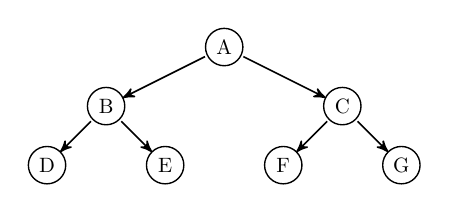
\begin{tikzpicture}[scale=0.75,transform shape]
  \tikzstyle{LabelStyle}=[fill=white,sloped]
%  \tikzstyle{EdgeStyle}=[bend left]
  \Vertex[x=0,y=0,LabelOut=false]{A}
  \Vertex[x=-2,y=-1]{B}
  \Vertex[x=2,y=-1]{C}
  \Vertex[x=-3,y=-2]{D}
  \Vertex[x=-1,y=-2]{E}
  \Vertex[x=1,y=-2]{F}
  \Vertex[x=3,y=-2]{G}
  \tikzstyle{EdgeStyle}=[post]
  \Edge[](A)(B)
  \Edge[](A)(C)
  \Edge[](B)(D)
  \Edge[](B)(E)
  \Edge[](C)(F)
  \Edge[](C)(G)
%  \Edge[label=$$](K)(F)
\end{tikzpicture}
\caption{\label{fig:arborescence}Arborescence}
\end{figure}

The arborescence\cite{arborescence} is a simple tree structure defined by having exactly one directed path from the root node to every other node in the tree. It supports each node having a number of children which may themselves have a number of children. This expresses the property of a single identity (the parent node) being able to act through multiple identities (the child nodes). Note also that, as alluded to earlier, each child node is itself an identity, qualitatively equivalent to the parent identity in every way. Therefore, this identity representation could extend an arbitrary number of levels, endlessly bifurcating all the way down.

\subsection{Polytree} \label{sec:polytree}

\begin{figure}[htp]
\centering
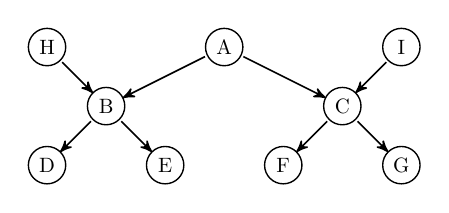
\begin{tikzpicture}[scale=0.75,transform shape]
  \tikzstyle{LabelStyle}=[fill=white,sloped]
%  \tikzstyle{EdgeStyle}=[bend left]
  \Vertex[x=0,y=0,LabelOut=false]{A}
  \Vertex[x=-2,y=-1]{B}
  \Vertex[x=2,y=-1]{C}
  \Vertex[x=-3,y=-2]{D}
  \Vertex[x=-1,y=-2]{E}
  \Vertex[x=1,y=-2]{F}
  \Vertex[x=3,y=-2]{G}
  \Vertex[x=-3,y=0]{H}
  \Vertex[x=3,y=0]{I}
  \tikzstyle{EdgeStyle}=[post]
  \Edge[](A)(B)
  \Edge[](A)(C)
  \Edge[](B)(D)
  \Edge[](B)(E)
  \Edge[](C)(F)
  \Edge[](C)(G)
  \Edge[](H)(B)
  \Edge[](I)(C)
%  \Edge[label=$$](K)(F)
\end{tikzpicture}
\caption{\label{fig:polytree}Polytree}
\end{figure}

The polytree\cite{polytree} is a more general model than the arborescence and allows a node to have multiple parents. This expresses the property of an identity being comprised by multiple identities. We call such an identity a \textit{hive identity} or a \textit{composite identity} (these are relative terms). Human institutions such as marriage, nations, and corporations are such identities. Ant colonies, bee hives, starling murmurations are such identities. So indeed are physical atoms, chemical molecules, and living cells.

\subsection{Multitree} \label{sec:multitree}

\begin{figure}[htp]
\centering
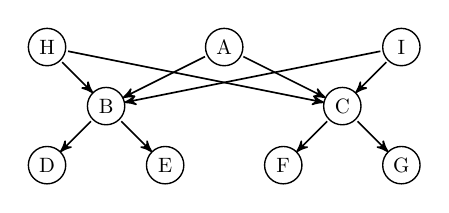
\begin{tikzpicture}[scale=0.75,transform shape]
  \tikzstyle{LabelStyle}=[fill=white,sloped]
%  \tikzstyle{EdgeStyle}=[bend left]
  \Vertex[x=0,y=0,LabelOut=false]{A}
  \Vertex[x=-2,y=-1]{B}
  \Vertex[x=2,y=-1]{C}
  \Vertex[x=-3,y=-2]{D}
  \Vertex[x=-1,y=-2]{E}
  \Vertex[x=1,y=-2]{F}
  \Vertex[x=3,y=-2]{G}
  \Vertex[x=-3,y=0]{H}
  \Vertex[x=3,y=0]{I}
  \tikzstyle{EdgeStyle}=[post]
  \Edge[](A)(B)
  \Edge[](A)(C)
  \Edge[](B)(D)
  \Edge[](B)(E)
  \Edge[](C)(F)
  \Edge[](C)(G)
  \Edge[](H)(B)
  \Edge[](I)(C)
  \Edge[](H)(C)
  \Edge[](I)(B)
%  \Edge[label=$$](K)(F)
\end{tikzpicture}
\caption{\label{fig:multitree}Multitree}
\end{figure}

The multitree\cite{multitree} is a strengthening of the polytree, possessing only the constraint that no node can have parents that have a common ancestor, i.e. that there can be no set of nodes that form a ``diamond'' in the tree. This model expresses the ability of identities to form different child identities with the same parents. For example, two people can be friends as well as colleagues. As another example, the same set of chemical elements can form two different molecules, or isomers.

\subsection{``Identitree''} \label{sec:identitree}

\begin{figure}[htp]
\centering
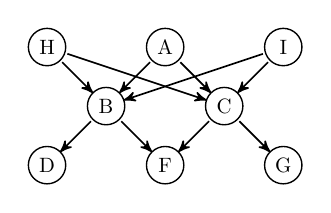
\begin{tikzpicture}[scale=0.75,transform shape]
  \tikzstyle{LabelStyle}=[fill=white,sloped]
%  \tikzstyle{EdgeStyle}=[bend left]
  \Vertex[x=0,y=0,LabelOut=false]{A}
  \Vertex[x=-1,y=-1]{B}
  \Vertex[x=1,y=-1]{C}
  \Vertex[x=-2,y=-2]{D}
  \Vertex[x=2,y=-2]{G}
  \Vertex[x=0,y=-2]{F}
  \Vertex[x=-2,y=0]{H}
  \Vertex[x=2,y=0]{I}
  \tikzstyle{EdgeStyle}=[post]
  \Edge[](A)(B)
  \Edge[](A)(C)
  \Edge[](H)(B)
  \Edge[](I)(C)
  \Edge[](B)(D)
  \Edge[](C)(G)
  \Edge[](B)(F)
  \Edge[](C)(F)
  \Edge[](H)(C)
  \Edge[](I)(B)
%  \Edge[label=$$](K)(F)
\end{tikzpicture}
\caption{\label{fig:identitree}Identitree}
\end{figure}

The identitree is a generalization of the multitree which eliminates the ``no-diamonds'' constraint. This enables identities that have common ancestors to unite. It may seem unclear why this sort of union would be needed, but consider that in the multitree model, two identities with only a single common ancestor, however distant, would be unable to unite. The identitree enables this union (which, as a clarification, does not refer to a biological relationship but a conceptual one).

\subsection{``Bodhitree''} \label{sec:bodhitree}

\begin{figure}[htp]
\centering
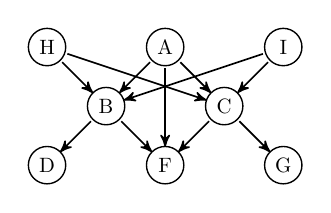
\begin{tikzpicture}[scale=0.75,transform shape]
  \tikzstyle{LabelStyle}=[fill=white,sloped]
%  \tikzstyle{EdgeStyle}=[bend left]
  \Vertex[x=0,y=0,LabelOut=false]{A}
  \Vertex[x=-1,y=-1]{B}
  \Vertex[x=1,y=-1]{C}
  \Vertex[x=-2,y=-2]{D}
  \Vertex[x=2,y=-2]{G}
  \Vertex[x=-2,y=0]{H}
  \Vertex[x=2,y=0]{I}
  \Vertex[x=0,y=-2]{F}
  \tikzstyle{EdgeStyle}=[post]
  \Edge[](A)(B)
  \Edge[](A)(C)
  \Edge[](H)(B)
  \Edge[](I)(C)
  \Edge[](B)(D)
  \Edge[](C)(G)
  \Edge[](B)(F)
  \Edge[](C)(F)
  \Edge[](H)(C)
  \Edge[](I)(B)
  \Edge[](A)(F)
%  \Edge[label=$$](K)(F)
\end{tikzpicture}
\caption{\label{fig:bodhitree}Bodhitree}
\end{figure}

The only restriction in the identitree model is that an identity cannot unite with an ancestor node. The removal of this restriction results in the ``bodhitree,'' which it can be shown is topologically equivalent to an acyclic graph\footnote{While structurally the bodhitree is equivalent to an acyclic graph, we will employ the term bodhitree when discussing identity trees specifically as opposed to more general graphical depictions such as of network connectivity. Thus in application the bodhitree has an implicit notion of causality, and so as a convention, and in contrast to an acyclic graph, all edges flow in a particular direction to depict this (of course, there could be alternate depictions that capture this). It is our hope as the models for identity are further developed, that bodhitree representations (pictorial and otherwise) will continue to incorporate these developments in order to convey information most usefully.}. The ability to unite with an ancestor node seems of questionable value, but consider that in the other models with such a restriction in place, descendants are distinguished in the context of ancestors, violating our requirement for all identities to be qualitatively equivalent. We will return to this after further elaborating the mathematical model for identity. Let us first formalize the above development in precise definitions. Note that the bodhitree/acyclic graph is the most general model, with each preceding one above being a further specialization.

\begin{defn}
	A \emph{graph}\footnote{We will assume graphs are directed unless otherwise specified. Since undirected graphs may be modeled by directed graphs by treating edges as the unordered pair of directed edges $\{(u,v),(v,u)\}$\cite{chartrand}, directed graphs may be seen as a more general model, which motivates our choice of terminology.} $\Gamma$ is an ordered pair $(V, E)$ consisting of a finite nonempty set $V$ together with an irreflexive relation $E$ \cite{chartrand}. The elements of $V$ are called \emph{vertices}, or \emph{nodes}, and the elements of $E$ are ordered pairs of vertices called \emph{edges}. A (directed) sequence of linked edges connecting one vertex to another is called a \emph{path}.
	\begin{equation}
		\begin{split}
			\Gamma &= (V, E) \text{, where} \\
			V &\neq \varnothing \text{, and } E \subset V \times V \mid \\
			(u,v) \in E &\implies (v,u) \notin E \text{, and} \\
			(u,u) &\notin E \,\, \forall u \in V .
		\end{split}
		\nonumber
	\end{equation}
\end{defn}

\begin{defn}
	An \emph{acyclic graph}, or \emph{bodhitree}, is a graph such that $E$ does not contain a path from some vertex $u$ to itself.
\end{defn}

\begin{defn}
	An \emph{identitree} is a bodhitree such that if $(u, v) \in E$, then there is no path in $E - \left\{\left(u, v\right)\right\}$ originating at $u$ and terminating at $v$.
\end{defn}

\begin{defn}
	A \emph{multitree} is a bodhitree such that for any vertices $u, v \in V$, if a path exists between them then it is unique. Any multitree is also an identitree.
\end{defn}

\begin{defn}
	A \emph{polytree} is a bodhitree such that for any vertices $u, v \in V$, there is a unique undirected path (i.e. ignoring the ordering on the edges) between them. Any polytree is also a multitree.
\end{defn}

\begin{defn}
	An \emph{arborescence} is a polytree containing a least element in $V$ (``root'' vertex) with respect to the natural ordering on edges.
\end{defn}

\section{Mathematical Model} \label{sec:matmod}

\subsection{Foundations} \label{sec:foundations}

The models above characterize our high-level intuitions of the behavior of identity. Now we develop a mathematical foundation on which to base further development of the model.

Let's collect some observations, following which we'll develop the model:

\begin{enumerate}
	\item Identities must exist ``somewhere,'' i.e. within some ``context'' whose nature is to be elaborated.
	\item Since identities ought to be a universal model, it follows that anything that can be considered to ``exist'' in some context must be an identity in that context.
	\item All identities are qualitatively equivalent (and together with intuitions discussed earlier this appears to imply the bodhitree model above).
\end{enumerate}

Due to the fractal nature of identity architecture, the definitions below may sometimes reference ideas that have not yet been defined, and which are then defined later. This apparent circularity can be resolved by imagining that at the level of each definition, the referenced concepts are either at a ``lower'' or ``higher'' level as the case may be, and as such are assumed to simply have been provided beforehand, similar to the case of set theory where the elements of sets are themselves sets. Finally, many of the axioms below are intended to be superseded in the framework of Epistemic Priority described in \autoref{sec:epipri}.

\begin{defn}[Identity Context] \label{def:idecon}
	An \emph{identity context}, or simply \emph{context}, is a universe $\mathcal{W}$ of identities (which for now can be thought of as sets) such that:
	\begin{itemize}
		\item There exists an identity with no ancestors: $\exists \varnothing_W \in \mathcal{W}$ (\emph{Axiom of Existence/Anonymous Identity})
		\item If $x, y \in \mathcal{W}$, then $\exists q \in \mathcal{W} \mid \{x,y\} \twoheadrightarrow q$ (\emph{Axiom of Hive Identity}\footnote{Corresponds to the Axiom of Pairing in set theory.})
		\item If $x \in \mathcal{W}$ and $y \twoheadrightarrow x$, then $y \in \mathcal{W}$ (\emph{Axiom of Transitivity})
		\item If $x \in \mathcal{W}$, then $\exists q \in \mathcal{W} \mid \mathscr{P}(\chi(x)) \twoheadrightarrow q$ (\emph{Axiom of Power Identity}\footnote{Corresponds to the Axiom of Power Set in set theory.})
		\item If $J \in \mathcal{W}$ where $J$ is a set, and $\{x_{\alpha}\}_{\alpha \in J}$ is a family of constituents of $\mathcal{W}$, then $\exists q \in \mathcal{W} \mid \bigcup_{\alpha \in J} {\chi(x)}_{\alpha} \twoheadrightarrow q$ (\emph{Axiom of Union});
	\end{itemize}
	where $\chi$ is a function on $\mathcal{W}$ mapping each identity to the set of its parents; $x \twoheadrightarrow y$ denotes that $x$ is a parent of $y$, i.e. $x \twoheadrightarrow y \iff x \in \chi(y)$; and the notation $\{x,y\} \twoheadrightarrow q$ is shorthand for ``$x \twoheadrightarrow q$ and $y \twoheadrightarrow q$.'' These axioms for sets define a \emph{Grothendieck Universe}\cite{grothendieck}\cite{foundcat}, a foundational construct in mathematics. In the terminology from set theory, subsets of $\mathcal{W}$ are called \emph{classes}. If a class is not itself a set in the universe, then it is called a \emph{proper class}.
	Note that defining the identity context this way naturally entails a bodhitree hierarchy of identities (under the relation of constitution, $\twoheadrightarrow$), as desired. Additionally, this characterization allows us to consider an identity context as a \emph{category of identities} (in the category theoretic sense).
\end{defn}

\begin{defn}[Axiom of Worlds]
	For any conceivable entity $Q$, there exists a context $\mathcal{W}$ such that $Q$ is an identity in that context\footnote{This is analogous to the ``axiom of universes''\cite{maclane} in set theory, esp. in connection with grothendieck universes.}.
	\begin{equation}
		\forall Q \; \exists \mathcal{W} \mid Q \in \mathcal{W}. \nonumber
	\end{equation}
	In particular, this axiom guarantees the existence of a context $\mathcal{W}$ such that a proper class in a given context constitutes an identity in $\mathcal{W}$.
\end{defn}

\begin{defn}[Constituent]
	Identities that actually manifest in a context $\mathcal{M}$ (from the possible identities allowed in the universe) will in general be called \emph{constituents} or \emph{members}. ``$x$ is a constituent of $\mathcal{M}$'' will be denoted $x \in \mathcal{M}$.
\end{defn}

\begin{defn}[Body]
	The set $B$ of identities that form an identity $Q$ is called the \emph{body} of $Q$; i.e. $\chi(Q) = B$.
\end{defn}

\begin{defn}[Component]
	Elements of the body of an identity $Q$ will be called \emph{components} or \emph{features} of $Q$. ``$x$ is a component of $y$'' will be denoted $x \twoheadrightarrow y$.
\end{defn}

For any identity, there is the context to which it belongs (the ``outside'') and the context it defines (the ``inside''). We will formalize these notions:

\begin{defn}[World]
	Given an identity, the \emph{world} is defined to be the context within which it exists. Members of the world are called \emph{things}.
\end{defn}

\begin{defn}[Mind]
	Given an identity, the \emph{mind} is defined to be the context it defines. Members of the mind are called \emph{thoughts}.
\end{defn}

When considering a particular pair of contexts entailing a mind/world relationship, we will denote the mind by $\mathcal{M}$ and the world by $\mathcal{W}$. If it becomes necessary to consider outer worlds beyond $\mathcal{W}$ or inner minds within $\mathcal{M}$, we will denote these by $\mathcal{W}_0$, $\mathcal{W}_1$, $\mathcal{W}_2$ \ldots, going outward, and $\mathcal{M}_0$, $\mathcal{M}_1$, $\mathcal{M}_2$ \ldots, going inward, with $\mathcal{M}$ and $\mathcal{W}$ without further qualification taken to mean $\mathcal{M}_0$ and $\mathcal{W}_0$ respectively. ``Thoughts'' and ``things'' are relative terms associated with a particular choice of mind/world boundary: things in one world may well be treated as thoughts in relation to an outer world.

\begin{defn}[i-morphism]
	For identities $(X, \phi)$ and $(Y, \psi)$, an \emph{i-morphism} from $X$ to $Y$ is a mapping $f : X \rightarrow Y$ such that for $x_1, x_2 \in X$,
	\begin{equation}
		f(\phi(x_1)(x_2)) = \psi(f(x_1))(f(x_2)) ,
		\nonumber
	\end{equation}
	where $\phi$ and $\psi$ are the actions (defined below) of the identities $X$ and $Y$ respectively.
\end{defn}

For example, if $(X, \phi)$ is a group, then under an i-morphism $f$, $(f(X), \psi)$ would be a group as well. The i-morphism can be seen as an abstraction of the ideas of monoid homomorphism, group homomorphism, ring homomorphism, and so on, and closely related to (but not quite the same as) the categorical notion of ``morphism.''

For an identity $(X, \phi)$ we can define a set of $\phi$-endomorphisms on $X$ consisting of all i-morphisms $X \rightarrow X$. We will denote this set of $\phi$-endomorphisms by $\hom(X, X)$.

\begin{defn}[Identity Action]
	An \emph{identity action}, or simply \emph{action} of an identity $(A, \phi)$ on an identity $(B, \psi)$ is an i-morphism
	\begin{equation}
		\rho : A \rightarrow \hom(B,B) ,
		\nonumber
	\end{equation}
	from $A$ to the set of $\psi$-endomorphisms on $B$. It will be denoted $A \odot B$ (it's an ``eye'').

	Every action of $A$ on $B$ gives rise to a reaction -- an action of $B$ on $A$. This, in turn, being an action itself, gives rise to a reaction from $A$, and so on, recursively. This reaction sequence is said to terminate when an action equals the trivial action. We can call such a sequence an \emph{interaction}. The action of $A$ on $B$ translates, in the mind of $B$, into interactions between the constituents of $B$, and so on.
\end{defn}

The identity action, couched in formalism though it is, is an intimately intuitive notion. The idea is that when we manipulate anything in the world around us, that manipulation is a relationship between the understanding of that object we possess in our mind and the set of all possible transformations (``endomorphisms'') of that object in the world. In other words we are able to change the world around us (including our bodies as members of the world) in ways that we understand how to do in our minds (note that this doesn't imply that the result conforms to our understanding -- only the manipulation), and within the bounds of what's possible in the world. The identity action captures and generalizes this notion. Mathematically, it can be seen as an abstraction of the notions of ``group action,'' ``monoid action,'' ``ring action,'' and so on, with each of these notions being treated as specific instances. This is developed further in \hyperref[app:algact]{appendix}.

As a further clarification, note that the reaction sequence described here is a deterministic consequence of the initial action and of the nature of the identities involved, and does not refer to any subsequent action on the part of the other identity which may be entailed in the conventional sense of the word ``reaction'' -- such an action would be a distinct action. The algebraic relationship between action and reaction remains to be specified in future work.

The action of a hive identity can be specified directly in terms of the actions of its constituents. There is an antecedent result for sets that the action of a family of sets $(\Omega_i)_{i \in I}$ on a set $E$ can be specified as an action of the disjoint union of the $\Omega_i$ that extends each of the actions of the $\Omega_i$ on $E$\cite{bourbaki}. This can be seen to be a special case derivative of the more general categorical construction of \emph{coproduct} (of which the disjoint union is an instance, in the category of sets), and we can consider the action of a hive identity to be an action of a form of coproduct (i.e. one that generalizes the coproduct construction in terms of i-morphisms and not just (categorical) morphisms all of the same type) of all of its constituents. This specification is left to be developed in future work.

\begin{defn}[Identity]
	In a world $(\mathcal{W}, \psi)$, an \emph{identity} $Q$ is a tuple $(\mathcal{M}, B, \phi, \mu, \omega)$ where $\mathcal{M}$ is an identity context provided by the Axiom of Worlds (the \emph{mind}\footnote{The mind context here is obtained via invocation of the Axiom of Worlds in relation to the world $\mathcal{W}$ as an identity, as an implied generalization from the fact that ``the world'' is conceivable as a thought in a human mind, whereas the world contains no representation of a human mind except in other (human) minds \emph{associated} with the world.}), $B$ is the set of identities in $\mathcal{W}$ that form $Q$ (the \emph{body}), $\phi$ is an identity action, $\mu : \mathcal{W} \rightarrow \mathcal{M}$ is a free functor (the ``\emph{perception functor}''), and $\omega : \mathcal{M} \rightarrow \mathcal{W}$ is a forgetful functor (the ``\emph{expression functor}'') such that for $T \in \mathcal{M}$ and $G \in \mathcal{W}$:
	\begin{equation}
		\begin{split}
			\omega(\phi(T)(\mu(G))) &\naturalto \psi(\omega(T))(G) \text{ and} \\
			\mu(\psi(G)(\omega(T))) &\naturalto \phi(\mu(G))(T)\text{,} \\
			\text{i.e. } \omega(T \odot_{\mathcal{M}} \mu(G)) &\naturalto \omega(T) \odot_{\mathcal{W}} G \text{ and} \\
			\mu(G \odot_{\mathcal{W}} \omega(T)) &\naturalto \mu(G) \odot_{\mathcal{M}} T .
		\end{split}
		\nonumber
	\end{equation}

	\begin{center}
		\begin{tikzcd}
			\mathcal{W} \arrow{d}{\mu} \arrow{rd}[inner sep=1pt]{1_{\mathcal{W}}}[name=T,below]{} & & & \mathcal{M} \\
			\mathcal{M} \arrow{r}{\omega} \arrow[Rightarrow, to path=-- (T) \tikztonodes]{}{} & \mathcal{W} & \mathcal{M} \arrow{r}{\omega} \arrow{ru}[inner sep=1pt]{1_{\mathcal{M}}}[name=S,below]{} & \mathcal{W} \arrow{u}{\mu} \arrow[Rightarrow, to path=-- (S) \tikztonodes]{}{}
		\end{tikzcd}
	\end{center}

	where $\naturalto$ represents a natural transformation. $\mu$ and $\omega$ can thus be seen to constitute a form of categorical equivalence (in the sense of category theory) between the mind and the world, and in particular an adjunction (the ``\emph{mind/world adjunction}'') $\mu \dashv \omega$.
\end{defn}

If $\mu$ and $\omega$ form an isomorphism, then the mind is said to be \emph{transparent} and in this case the body could be identified with the mind. For discussion of mathematical objects we will generally assume that the mind is transparent. The nature of the action characterizes, and is characterized by, the nature of the identity. For example, if the action of an identity $Q$ is simply the trivial mapping of $B \rightarrow \hom(B,B)$, then this identity $Q$ is simply a set. With additional specification of the action, the identity is developed into more sophisticated structures such as monoids, groups, rings, etc. (\hyperref[app:algact]{appendix}), or even more complex structures that could serve as models for things in our experience that are not obviously algebraic.

We may often speak of minds ``in'' a world, or minds ``within'' a world, as this usage is natural and captures a useful intuition; however the terms do not strictly imply ``containment'' in the usual sense. As a philosophical note, ``existence'' is \textit{defined} as an identity in a context, thus, to say that a mind is ``in'' a world may suggest that the mind is an identity in that world, but in fact the mind itself is not -- only the identity with which it is associated is. Thus a mind being ``in'' a world should more precisely be interpreted as a mind being ``associated'' with that world, or alternatively, ``the identity whose mind this is'' being in that world. The world does provide the dialectical context that all minds associated with that world share, and the ``in'' usage captures this aspect of containment. On the other hand, the world (as a whole) in fact is (i.e. corresponds to) an identity in the mind, as deriving from the Axiom of Worlds and the definition of Identity.

\begin{lemma}[Maya] \label{lem:maya}
	With respect to identities $Q_i = (\mathcal{M}_i, B_i, \phi_i, \mu_i, \omega_i)$ in a world $\mathcal{W}$:
	\begin{center}
		$x \in \mathcal{W} \implies \mu_i(x) \in \mathcal{M}_i \; \forall i$
	\end{center}
	``Things in a world are represented as thoughts in every mind within that world.'' On the other hand, in general thoughts do not exist independently as things.\footnote{The name references the Vedantic concept of \emph{M\={a}y\={a}}, which does not refer in particular to mental representation of an external world, but more abstractly to conscious epistemic representation of true reality, for which mental representation of the physical world is often used as a metaphor in Vedantic works, and which may be treated as a specific manifestation of maya. Since the present lemma does not apply specifically to human minds associated with the physical world but to mind and world abstractly, it is largely in the spirit of the Vedantic conception.}
\end{lemma}

\begin{corollary}[Decidability] \label{cor:decidability}
	Assertions that are true or false in the mind are in general undecidable in the world (e.g. via dialectical method).
\end{corollary}

\subsection{Dynamics} \label{sec:dynamics}

A blues band gets together to have a jam session in the apartment of one of the band members. The drummer counts them off and they begin a funky improvisation. They're feeling the groove, each member playing off of the ideas that emerge in their music. Their activities also affect other things in their immediate surroundings, such as the sound resonating with furniture and cavities in the room. The smooth bassline travels through the walls and reaches the ear of one of the crotchety neighbors, who registers mild annoyance and reluctant enjoyment. The music is faintly audible outside the building and alters the course of a few dust particles in the air outside. The band members are also visible through a window, the light from which travels outward and has distant insignificant interactions in the surrounding universe.

The above can be seen as an example of \emph{genesis}.

\begin{defn}[Genesis]
	Genesis is a computation associated with the manifestation of an identity within a context. For a family of identities $(q_{j})_{j \in J}$ in a world $\mathcal{W}$, an action $\odot (q_{j})_{j \in J}$ implicitly defines a mind context in which the transformed (under $\odot$) identities $q_{j}'$ reside, which corresponds to a new identity $Q_{0} = (\mathcal{M}_{0}, \phi_{0})$. The action $\odot$ on each of the constituents $q_{j}$ factors internally within their minds as interactions between the thoughts of the $q_{j}$. The action also affects other identities in the world to different extents, which can be abstracted as a hive action of $Q_{0}$ on a subset of $\mathcal{W}$ to form, relative to each constituent $i$ in that subset, a mind $Q_{i} = (\mathcal{M}_{i}, \phi_{i})$ containing $Q_{0}$ to the extent of the action of $Q_{0}$ on $i$. In this manner, the computation continues generating constituent-relative containing minds and terminates at the stage where the action of $\odot$ on $\mathcal{W}$ is trivial, at which stage there exists a ``terminal'' mind $Q = (\mathcal{M}, \phi)$ containing all the $Q_{i}$ as thoughts. Note that each action entailed in the computation germinates an interaction.
\end{defn}

\begin{defn}[Somatic]
	The members of a world that initiate genesis of an identity correspond to the \emph{somatic} constituents in the mind of that identity in relation to that world (since they form the body of the identity in the world as defined earlier).
\end{defn}

\begin{proposition}
	Descendants in a bodhitree are structurally related to ancestors.
\end{proposition}

\begin{corollary}[``Law of Karma'']
	Effects are structurally related to causes.
\end{corollary}

These can be derived from the definition of identity action and the nature of genesis.

Chester\cite{chester} has previously motivated an algebraic characterization of identity, observing that the symmetries of an object (in the sense of group theory) as ``sameness under altered scrutiny'' characterize the identity of that object with respect to the observer, and that groups therefore characterize identity in some sense. We could interpret this in our model to mean that one's ``description'' of an identity, being an identity tree, is invariant under alternate description. That is, the same identity with respect to a particular observer may be described in multiple ways, but the bodhitrees corresponding to the different descriptions must be equivalent in some algebraic sense, forming a group. This description could be said to correspond to the \emph{information} the observer has about a particular identity. Additionally, the image of the action of $a$ on $b$ by definition conveys some of the structure of $a$ to $b$, and it is to this extent that $a$ exists in the $b$-relative mind. We can interpret this as a conveyance of information from $a$ to $b$.

Muller\cite{muller} proposes a unification of all forms of entropy (information) as derivative of group structure via the Cauchy-Frobenius-Burnside Lemma:

\begin{equation}
	I = \log\biggl(\frac{1}{|G|} \sum_{g \in G} S^{g}\biggr) ;
\end{equation}

where $I$ is the information conveyed (e.g. in bits, if the base of the logarithm is chosen to be $2$), and the parenthetical expression is the number of orbits under the action of the group $G$ on a set $S$, given by Burnside's lemma. If the action of an identity $a$ on an identity $b$ can be interpreted as a group action (i.e. a group homomorphism to the automorphisms of $b$), then the applicability of Burnside's Lemma would immediately follow to give us a candidate amount of entropy conveyed from $a$ to $b$, in the sense of Muller. But if the action is not a group action, then the amount of information conveyed may need to be derived from some natural group characterization of the image of the action (possibly involving free groups or Grothendieck groups\cite{grogroup}). Alternatively, it's possible such an information-theoretic characterization may be accomplished using ``logical entropy'' as described by Ellerman\cite{ellerman} or by following the program described in Devlin\cite{devlin}.

\textit{For the remainder of this document, we will generally speak in terms of ``absolute'' contexts for which the constituents are fixed and each constituent is aware of all actions performed within that context. Although in nature contexts are to be considered relative to each observer as described above, employing such an ``absolute'' characterization will allow us to explore idealized properties of identities and contexts without getting lost in the dynamical details.}

\section{Anonymous Identity} \label{sec:anoide}

\subsection{An Illustrative Example} \label{sec:illexa}

Consider the following three variations on a particular situation:

\paragraph{}

Alice walks into an elevator and, having eaten a heavy meal of beans for lunch, feels a tightness in the abdomen and decides to let one rip. Good thing no one else is around, she thinks to herself.

\paragraph{}

Alice and Bob walk into an elevator having both eaten large helpings of beans at lunch. One of them can't hold back and decides to let one go. They both avoid eye contact as Bob knows he did it, and Alice knows he did too.

\paragraph{}

Alice, Bob, and Carol walk into an elevator having all had heaping servings of beans for lunch. They knew they'd have to pay the price eventually but all they could think of over lunch was how yummy the beans were. Fate comes to collect an early fare from one of them, and they can't help but deliver a slow, silent-but-violent dose to the assembled gentry. Alice looks at Bob, who returns an amused and knowing look. They glance surreptitiously at Carol who smiles at them both in a vaguely accusing manner as if to say, ``He who smelt it, dealt it.'' They all walk out without saying a word. Presumably one of them knows who did it, but it is a secret they will take to the grave.

\subsection{Origin of Anonymous Identity} \label{sec:orianoide}

The example above illustrates a simple truth -- anonymity cannot exist if there are fewer than three interacting identities. If there are only two people in the elevator there can be no doubt as to the identity of the perpetrator of flatulence. But with three people, suddenly it's impossible to tell. \textit{Anonymity begins at $3$}. 

This fact could explain why the institution of marriage between two people has been so successful and persistent through the ages. From an identity perspective, it's the maximum number of somatic constituents you could have while still being able to achieve perfect fidelity of information across the constituents. Each partner in the pair knows their own activities, and by virtue of knowing which of the pair's activities are not their own, they also know fully the activities of the partner (in the idealization).

\begin{figure}[htp]
	\centering
	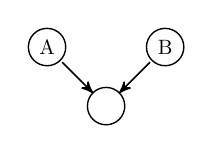
\begin{tikzpicture}[scale=0.75,transform shape]
		\tikzstyle{LabelStyle}=[fill=white,sloped]
		%  \tikzstyle{EdgeStyle}=[bend left]
		\Vertex[x=-1,y=0,LabelOut=false]{A}
		{
			\SetVertexNoLabel
			\Vertex[x=0,y=-1]{C}
		}
		\Vertex[x=1,y=0]{B}
		\tikzstyle{EdgeStyle}=[post]
		\Edge[](A)(C)
		\Edge[](B)(C)
		%  \Edge[label=$$](K)(F)
	\end{tikzpicture}
	\caption{\label{fig:marriage}Marriage}
\end{figure}

Now some cultures sustain polygamous marriages, and apparently these are functional enough to have persisted over the centuries. How can this be? We will discuss this in the section on \hyperref[sec:phirelhistra]{\textit{religious traditions}}.

\subsection{Nature of Anonymous Identity} \label{sec:natanoide}

When an anonymous act is performed within the mind of an identity $Q$, by definition it is an act for which no member will claim responsibility. Therefore it is unknown which of the known constituents of the mind was responsible for the act. But at the same time, clearly \textit{somebody in $Q$} did it. How can this be captured? Consider a simple $3$-member identity where an anonymous act $X$ has been performed (Fig.~\ref{fig:anonymous}). Identity $A$ knows it didn't perform the act and so models it as derivative of the composite of $B$ and $C$. Say $C$ didn't perform the act either, so $C$ models it as derivative of the composite of $A$ and $B$. $B$ actually performed the act, but since it is not accepting responsibility for it, $B$ must within the mind of $Q$ model the act as derivative of the composite of $A$ and $C$. None of the models agree, and they can argue till the end of the world who was responsible for what, but there's simply no way to know who is ``lying'' and who isn't. Instead, the only way the models can be consistent is if the act is agreed to have been performed by the intersection of the three models $\{A, B\} \cap \{B, C\} \cap \{A, C\}$, which is the empty set. Therefore, anonymous acts are those corresponding to the empty set $\varnothing$ of identities, which is in line with our axiomatic definition of anonymous identity in \autoref{def:idecon}. Note that this is the empty subset within the mind of $Q$, which can as such still be identified with ``some identity in $Q$.'' In this regard it is to be treated as different from the empty subset in the world external to $Q$, in a sense soon to be made precise. As such, while in set theory the empty set is unique, here an anonymous identity (as with all identities) is defined with respect to a particular identity context (although the anonymous identity of a mind does correspond to the representation of the world anonymous identity in the mind under a perception functor). To highlight this distinction, and as a matter of notation, given an identity $Q = (\mathcal{M}_Q, B_Q, \phi_Q)$ in a world $\mathcal{W}$, we will denote the anonymous identity of the world by $\varnothing_\mathcal{W}$ and the anonymous identity of the mind of $Q$ by $\varnothing_{\mathcal{M}_Q}$ or simply $\varnothing_Q$. Finally, note that in the above interaction, all of the individual identities are aware of the ``true'' model from their perspective, and this is the model that they will use \textit{internally} -- that is to say, in their own mind contexts.

\begin{figure}[htp]
	\centering
	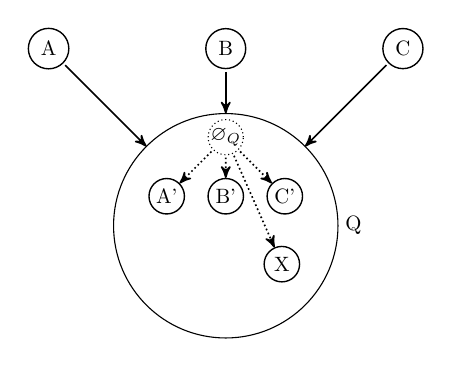
\begin{tikzpicture}[scale=0.75,transform shape]
		%\tikzstyle{LabelStyle}=[fill=white,sloped]
		%\draw[solid] (0,0) circle (2cm);
		\GraphInit[vstyle=Normal]
		\Vertex[x=-3,y=3]{A}
		\Vertex[x=0,y=3]{B}
		\Vertex[x=3,y=3]{C}
		{
			\tikzset{VertexStyle/.style = {draw=black,shape=circle,minimum size=3.8cm,inner sep=0pt}}
			\Vertex[x=0,y=0,LabelOut=true]{Q}
		}
		%\tikzset{VertexStyle/.append style = {draw=darkgray,text=darkgray}}
		{
			\tikzset{VertexStyle/.style = {draw=black,shape=circle,style=densely dotted,minimum size=0cm,inner sep=0pt}}
			\Vertex[x=0,y=1.5,L=$\varnothing_Q$]{QQ}
			%\tikzset{VertexStyle/.style = {draw=black,shape=circle,style=densely dotted,minimum size=0cm,inner sep=0pt}}
			%\Vertex[x=0,y=4.5,L=$\varnothing_W$]{WW}
		}
		{
			\tikzset{VertexStyle/.append style = {shape=circle,minimum size=0.6cm,inner sep=0pt}}
			\Vertex[x=-1,y=0.5,L=A']{A1}
			\Vertex[x=0,y=0.5,L=B']{B1}
			\Vertex[x=1,y=0.5,L=C']{C1}
			\Vertex[x=0.95,y=-0.65]{X}
		}
		\tikzstyle{EdgeStyle}=[post]
		\Edge[](A)(Q)
		\Edge[](B)(Q)
		\Edge[](C)(Q)
		{
			\tikzstyle{EdgeStyle}=[post,densely dotted]
			\Edge[](QQ)(A1)
			\Edge[](QQ)(B1)
			\Edge[](QQ)(C1)
			\Edge[](QQ)(X)
			%\Edge[](WW)(A)
			%\Edge[](WW)(B)
			%\Edge[](WW)(C)
		}
		%\tikzset{EdgeStyle/.append style = {draw=darkgray,text=darkgray}}
	\end{tikzpicture}
	\caption{\label{fig:anonymous}Anonymous Identity}
\end{figure}

A central notion in Vedanta philosophy is \emph{Brahman}, conceived to be the Absolute that inhabits and defines all reality. One particular argument used to demonstrate its conception is via the notion of \emph{mithya}, which denotes the ``dependent reality'' of a particular thing in relation to a more fundamental thing. For example, clay pots and jars are said to be mithya in relation to clay. In like manner, the argument goes, all existence is mithya in relation to Brahman. Furthermore, just as clay has fewer properties than objects made of clay, Brahman as the ultimate ground is said to be \emph{nirguna} -- having no properties whatsoever\cite{waite}. The notion so derived is essentially equivalent to anonymous identity in the present conception\footnote{As a ``historical'' note, anonymous identity did not initially have a basis in consciousness as Brahman does, which is the reason the concept was not developed in identification with the latter. They now share a compatible epistemic foundation.}. However, as should be evident from the definitions, anonymous identity does not carry any connotations of being ``absolute.'' In particular, in the example of clay and vessels made of clay, clay corresponds to the anonymous identity in the world of all things that can be made from clay. We may say that clay is the ``brahman'' of all things made from clay. Within the framework of identity architecture, the existence of an ``absolute'' brahman does not seem to be implied and, if held, must be treated as an axiom rather than as an implication of the argument.

It is nevertheless the case that in any context if we follow the known identity tree upward, we will eventually reach a set of identities for which there is no information about their genesis. These identities, following the reasoning outlined earlier, must also be modeled as anonymous acts, i.e. descended directly from the unique anonymous identity of the context. By considering the outermost world perceivable, we are led to conclude that all known identities must ultimately derive from the anonymous identity of that world\footnote{This is possibly related to the construction in set theory, via the cumulative hierarchy, of all sets in a Grothendieck universe by iterating set operations on the empty set.}, also depicted in Fig.~\ref{fig:anonymous}, and we may conceive this to be a ``relative brahman.'' Just as water takes the shape of any container, so does an anonymous identity -- or a brahman -- take the forms of all identities\footnote{Water may be seen to exhibit this property due to the fact that its shape (``no shape'') is the anonymous identity in the context of shapes. Thus anonymous identity provides the basis for this property of water (as a macro identity, not a molecule).}.

\begin{defn}[Anonymous Identity]
	Given a bodhitree $T$ and a set of identities $X$, a common ancestor $q$ of the $x_i \in X$ in $T$ is \emph{anonymous} in relation to them. Any act performed by $q$ is an \emph{anonymous act} in relation to $X$. Any hive with a body comprised entirely of such anonymous identities is itself anonymous in relation to $X$.
\end{defn}

\begin{defn}[Brahman]
	The unique supremum in $T$ in relation to the set $X$ corresponds to `the' anonymous identity or \emph{brahman} in the mind of a hive with body $X$. Since the supremum is not guaranteed to exist $n$ steps antecedent to the members of $X$ $\forall n$, the brahman may exist only as an infinite limit. Two such infinitary brahmans (e.g. in relation to two different sets of identities) in the same bodhitree need not necessarily be the same.
\end{defn}

These definitions formally justify why anonymity arises in the flatulence example described earlier -- ``an identity capable of flatulence'' is a common ancestor of the $3$ human identities in the elevator\footnote{This principle is also what allows us to blame the dog.}. The implied generalization is that \textit{any} such action that is derivative of a shared ancestor could conceivably be anonymous in this context, for example the presence of body odor, a human utterance, the pressing of elevator buttons (e.g. when others aren't looking), and so on.

\begin{proposition}[``Parable of the Fish'']\footnote{Referring to the ``parable'' told among physicists that in relation to fish, the ocean may be imperceptible or appear to have no properties due to the fact that it is present implicitly as the background of all things. But indeed the ocean does have properties (in relation to us) and is vastly complex. The suggestion is that we too may inhabit an ``ocean'' of sorts. A ``strong'' variation on this parable is that the ocean may be \emph{arbitrarily} complex and still be imperceptible to its inhabitants.}
	Given a bodhitree $T$ and a set of identities $X$, a common ancestor $q'$ of a common ancestor $q$ in relation to $X$ is indistinguishable from $q$ within the mind of $X$.
\end{proposition}

\section{Philosophical Conception} \label{sec:phicon}

\subsection{The Relationship between Consciousness and Reality}

So far we have described a mathematical framework within which a general abstraction of things and interactions may be represented, and have hinted at an underlying philosophical point of view. Let us now formally unravel this philosophical viewpoint.

Western philosophy has traditionally delineated two forms of knowledge: (1) \emph{empirical} knowledge, derived from the senses and our experience of the world, and (2) \emph{a priori} knowledge, not derived from the senses but nevertheless known. A priori knowledge was early conceived in a religious sense as ``preceding'' existence and being associated with a soul, but in more recent times starting with Locke\cite{russell}, this type of knowledge has increasingly been conceived in a ``weak'' sense -- ultimately deriving from experience even if not directly via perception. For example, mathematical abstractions derived inductively from empirical perception can be viewed as a priori in the modern (Kantian\cite{kant}) sense.

Still, the relationship between consciousness and experience is a subtle one, and it is worthwhile to investigate the evolution of thought on this particular point. Descartes\cite{descartes} explored this relationship by famously engaging in (what is now called) ``Cartesian doubt'' -- doubting everything, taking nothing for granted, and attempting to build one's entire edifice of knowledge from first principles. In doing so, he would observe that there were varying degrees of certainty that one could have about different types of knowledge: in particular, thought, he held, was more certainly ``true'' than the objects of the world. The argument (which would later be called ``the cogito'') that it is through thought that one infers one's existence in the world, ``I think, therefore I am,'' was the touchstone of his work.

A position of this sort is to be found in the Upanishads (foundational works in the Indian philosophical tradition). But instead of settling on a generalized conception of ``thought'' as the basis for reality as cogito does, the Upanishadic position was to take consciousness itself as the prime certainty, treating thought as simply another manifestation within consciousness qualitatively not much different from sensory perceptions. To mirror cogito's framing, it may be said that this position views ``I am'' to be the highest certainty\footnote{It is often stated as such, e.g. in \cite{brihadaranyaka}, but for the most part this view is foundational and tacitly assumed in subsequent development.}, and all other things as contingent in relation to it.

Although a subtle distinction, this turns out to have made all the difference; indeed, it turns the entire edifice of what we assume to constitute reality on its head. Formerly, as indeed in the present mainstream scientific viewpoint, consciousness is a phenomenon to be explained in terms of a presupposed substantial world -- how, we ask, does consciousness arise from a brain? But under the ``Consciousness First'' inversion, consciousness, possessing greater epistemic certainty than substance, need not be justified in relation to the latter. It is material things -- brains, for example -- that must be justified in relation to consciousness. What, we may ask, is the nature of a brain -- both as a substantial entity as well as an abstract one -- in relation to consciousness?

As a natural consequence of this inversion, philosophers in the Upanishadic tradition were evidently driven to study consciousness itself, directly, and they developed a systematic technique in order to do so -- the practice of \emph{dhy\={a}na}, or meditation\footnote{It is quite likely that either the practice of dhyana itself or some other similar contemplative practice preceded the philosophical inversion being discussed, and may have quite possibly led to it. It has also been suggested\cite{bronkhorst} that dhyana specifically (as opposed to other contemplative, ascetic practices) was discovered by Buddha.}. The direct study of consciousness is outside the scope of dialectical method (and by extension empirical\footnote{In the conventional, more-limited sense of `empirical' that we redefine as `dialectical' in the following section.} science) due in part to the dialectical undecidability (\autoref{cor:decidability}) that is inherent in such a study, but also due to other reasons which will be elaborated shortly. Given this, dhyana is a natural approach to the problem -- for when a phenomenon is to be studied ``scientifically'' it must first be isolated. This is precisely what dhyana achieves with regard to consciousness; all phenomena, perceptions, thoughts -- everything that is not consciousness itself -- are eliminated from experience in the practice of dhyana, so that what remains is consciousness alone, and one may then conduct experiments, so to speak, by perturbation of one's state of being by intuitive motion (or lack thereof). It is a little more than this, however, for eliminating phenomena from conscious experience does not merely isolate consciousness; it also brings into direct experience the very basis upon which those phenomena -- and reality more broadly -- are defined. Thus, dhyana is an epistemic notion in reality, a conceptual state of being, \textit{before it is anything else}.

Still, a priori, this need not get us anywhere. There seems to be no obvious basis against which we may expect that this approach need necessarily yield anything of value at all. It is, however, the testimony of practitioners throughout history -- to which this author must add his own -- that it does indeed yield results. Elaborate technical terminology is used in the meditative tradition to describe the various states of consciousness and the models that are proposed to account for them. Indeed, it appears to be the case that dhyanic insight forms the core of the entire Dharmic philosophical tradition, which could explain why it has proved difficult to integrate into the mainstream, containing as it does these ``mystical'' suggestions. Most of the schools of this tradition (including Buddhist, Jain, and Vedantic philosophy) seem to agree that there is a final insight or ``goal'' that is to be derived through the practice of dhyana and the cultivation of intellectual and intuitive insight. That goal is recorded to be \emph{Nirv\={a}\d{n}a} -- a purported liberation from empirical existence. The conceptions of this phenomenon differ in the various schools in subtle yet likely significant ways. Without addressing such theoretical conclusions at this stage, we propose to lay the groundwork for such a discussion, a framework within which the viability and significance of such ideas may be reckoned with.

\subsection{Categories of Knowledge} \label{sec:catkno}

In addition to the two categories of knowledge identified earlier, we may consider a third: knowledge derived via meditative insight. Buddhists appear to have referred to such knowledge as \emph{\={a}rya gy\={a}na}\cite{lankavatara}, meaning ``noble knowledge'' (often translated as ``Noble Wisdom'')\footnote{It is actually \emph{\={a}rya j\~{n}\={a}na}. We use the derivative ``gy'' found in modern Indic languages in place of ``j\~{n}'' as it is easier to pronounce.}. Additionally, consistent with this characterization, the Upanishads enumerate four ``states of consciousness'': (1) \emph{jagrat}, or waking, (2) \emph{svapna}, or dream, (3) \emph{sushupti}, or deep (dreamless) sleep, and (4) \emph{turiya}, literally the ``fourth'' state\cite{mandukya}. To achieve a similar level of comprehensiveness, and unifying these with the Western classification identified earlier, we sustain the categories: (1) empirical knowledge; derived from experience, and (2) a priori knowledge; not derived directly from experience but nevertheless known. Further, we propose that of these, empirical knowledge may be further subdivided into three categories: (1) dialectical knowledge\footnote{From dialectical in the sense of `dialogue': an abstract characterization of a type of knowledge (e.g. of the usual, waking world) that is defined in relation to more than one mind (e.g. in particular, other minds in addition to just that of the subject).}; the conventional ``empirical'' kind, derived from the conventional senses in the waking world and amenable to dialectical method, (2) dream knowledge; derived in dreams, and (3) aryagyanic knowledge; derived via intuitive, meditative apprehension. In line with Kant's broad conception of the a priori realm, we consider this realm to represent that in which all other types of knowledge may be related and synthesized. This conception is depicted in Fig.~\ref{fig:typesofknowledge}.

\begin{figure}[htp]
	\centering
	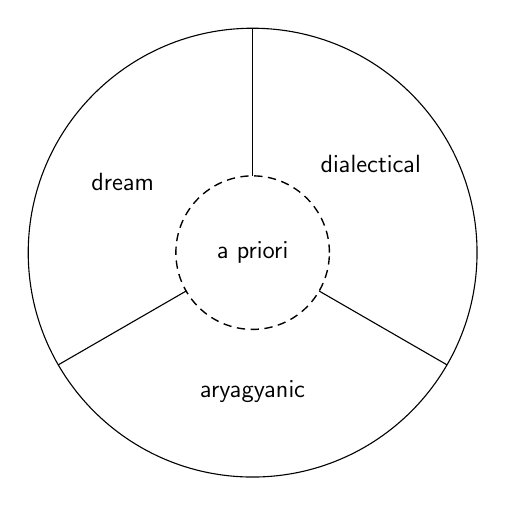
\begin{tikzpicture}[scale=0.75,transform shape]
		\GraphInit[vstyle=Normal]
		{
			\tikzset{VertexStyle/.style = {draw=black,shape=circle,minimum size=7.6cm,inner sep=0pt}}
			\SetVertexNoLabel
			\Vertex[x=0,y=0,LabelOut=true]{Q}
		}
		{
			\tikzset{VertexStyle/.append style = {shape=circle,style=densely dashed,minimum size=2.6cm,inner sep=0pt}}
			\Vertex[x=0,y=0,L=\large \textsf{a priori}]{Q'}
		}
		\draw (0,1.3) -- (0,3.8);
		\draw (1.126,-0.65) -- (3.291,-1.9);
		\draw (-1.126,-0.65) -- (-3.291,-1.9);
		\node at (2,1.5) {\large \textsf{dialectical}};
		\node at (-2.2,1.2) {\large \textsf{dream}};
		\node at (0,-2.35) {\large \textsf{aryagyanic}};
		%\node at (-1.7,-0.1) {\large \textsf{em-}};
		%\node at (-0.2,1.5) {\large \textsf{pi-}};
		%\node at (1.7,-0.3) {\large \textsf{ri-}};
		%\node at (0.3,-1.5) {\large \textsf{cal}};
	\end{tikzpicture}
	\caption{\label{fig:typesofknowledge}Types of Knowledge}
\end{figure}

The ``Consciousness First'' viewpoint was developed over a fruitful period of over a thousand years into what may be considered to be its logical conclusion: that it is not simply that consciousness has precedence over substance, but indeed that there is nothing else besides consciousness. This position is found in the \emph{citta-matra} (Consciousness-only or Mind-only) doctrine of Yogacara buddhism, and also in the conception of \emph{Brahman} in Advaita Vedanta as the Ultimate element -- \emph{sat-cit-ananda} (`existence-consciousness-bliss') -- that suffuses all reality\cite{waite}. Without commenting on the nuances of the doctrines of brahman or citta-matra, we assert that this general view -- ``Consciousness Only'' -- is the one we are inclined to adopt. That is to say, we take the position that \emph{consciousness is the ``stuff'' of nature and reality, and identity architecture either partially or completely accounts for its structure}.

Such ideas, while ostensibly philosophical, are also submitted as applying to the reality that is accessible to empirical investigation (in the broadened sense of empirical proposed above). Still, pushing as they do the boundaries of what is considered to be science, we feel it imperative to examine the foundations of what we consider to be knowledge and the standards by which different types of knowledge may be assessed. In doing so, we will examine what it means to know something, to what extent it can be asserted that something is known, and what sorts of questions are well-posed in an epistemic sense. Before we continue, we introduce a notion from buddhist philosophy known as \emph{ida\d{m}pratyayat\={a}} (translated as ``this/that conditionality''\footnote{This principle has such staggering applicability that a good English name for it might be ``Buddha's hammer,'' since in relation to it, ``every problem is a nail.''}). This notion entails the position that it is impossible to define anything in a vacuum; things are only defined in relation to something else. It is an abstract principle of relativity\footnote{Note that if we apply idampratyayata to the position that ``consciousness is the only reality,'' we must concede that consciousness is not well-defined except in relation to some complementary reality, and so an independently existing ``consciousness'' cannot be said to exist as such. This appears roughly to be the \emph{\.{s}\={u}nyat\={a}} (``emptiness'') position of Madhyamaka buddhism.}. For example, ``something'' and ``nothing'' are only definable in mutual reference to each other, and not independently\footnote{Additionally, it may be seen that ``nothing'' is simply an anonymous identity in relation to a given set of identities, that is to say a set of ``somethings,'' and is thus not conceived in an absolute sense.}.

\subsection{Epistemic Priority} \label{sec:epipri}

The notion of `truth' is subtle, and manifests differently in the a priori and dialectical realms. In the former, it has the character of being mathematical in nature, axiomatically founded, and logically proved. That is, propositions are demonstrated as true by way of logical inference from propositions that have already been demonstrated as true using the same mechanism. At the foundation we are forced to admit axioms -- propositions that are \emph{defined} to be true and are not provable. Without loss of abstraction, we could take these foundations of a priori truth to be the axioms of set theory together with axioms for logical inference. The most commonly adopted set-theoretic axioms are the ten Zermelo-Fraenkel-Skolem axioms including the Axiom of Choice, collectively known as the ZFC axioms. Set theory is built up from these ten axioms, and with additional axioms, higher structures are introduced such as groups, fields, topologies, and so on. All of these mathematical structures and their properties are `true' by virtue of logical consistency with the axioms.

In the dialectical realm, truth applies not to propositions themselves (which are constructed in the a priori realm and are therefore subject to the notion of truth in that realm) but to the \emph{correspondence} between a priori true models and the things they purport to model. Kant in his conception of ``noumena'' -- things as they are in themselves, prior to perception and categories of human understanding -- suggested that the noumena are in some sense forever outside our understanding: to the extent that they exist independently of our perception, nothing can be said about them that does not involve our (relational) understanding of them. This is a subtle idea with many interpretations. In one interpretation, the notion appears to describe something that exists without relation to anything else, which, by admitting idampratyayata, is not a well-defined conception. But noumenon is also interpreted in a different sense, as a \emph{limiting} conception which is the basis for the perceived entity. As Kant says, ``though we cannot know these objects as things in themselves, we must yet be in a position at least to think them as things in themselves; otherwise we should be landed in the absurd conclusion that there can be appearance without anything that appears.''\cite{kant} This is a key idea in relation to the dialectical world, that while our knowledge of noumena may be taken to increase to any arbitrary extent, there is no basis for the assertion that our a priori models are \emph{true} about them. We may say that dialectical truth is \emph{noumenal} in this sense. This noumenal undecidability may be seen, for example, in the inability of ``induction by enumeration'' to establish that, just because a correspondence between a model and a phenomenon has been observed to hold in $N$ instances, that it must necessarily hold on the $N+1$th instance\cite{russell}. On the other hand, it can be argued that we may conclude from a single instance of failure that the correspondence is false. Thus we may only determine whether our a priori models are \emph{false} or \emph{undecidable} (i.e. not yet shown to be false) in their correspondence with noumena\footnote{Although, the observation that a correspondence is false itself constitutes a dialectical assertion, and thus seemingly subject to the same undecidability as the original noumenal correspondence under consideration. This ``Hofstadter loop'' in scientific method is no doubt of importance and ought to be further specified in future work. Also along these lines, as intimated earlier it is likely that the mind should be treated as a context provided by the Axiom of Worlds, and in particular, the `world' (considered as a whole) exists as an identity, i.e. a thought, in the mind. It would then seem to be the case that noumenal undecidability of the dialectical world follows from mind/world undecidability with the world being treated as a mind in the mind.}. In the latter case, the truth of the correspondence may be adopted as an \emph{axiom}. This may be seen as justification for Popper's\cite{popper} falsifiability as an essential requirement in (dialectical) scientific investigation, that due to the noumenal nature of truth in the dialectical realm, \emph{dialectical} theories that are not falsifiable are forever outside our already constrained powers to evaluate.

In any case, our a priori edifice of truth is a key structure in founding truth and knowledge, to whatever extent these may be conceived. How the axioms upon which it is founded are chosen is therefore an important point. At present the axioms are conventional in nature, conforming to common sense and intuition, and largely possessing a self-evident quality that makes them unobjectionable. Still, in the event a contradiction were ever discovered, what would be the criteria on which to judge which axioms to keep? There are none. We may say that all of the axioms have roughly the same ``epistemic priority,'' that is, they are equals in their role as constituting the foundation of mathematics, and more generally, of a priori truth. Perhaps as an alternative to this, our epistemic foundations may be laid a different way such that, in a Cartesian sense, different priorities may be assigned to axioms as having greater or lesser certainty than others. We sketch one such possible axiomatic basis below. Note that by their very nature these axioms must take the form of ``affirmations.'' Note also that the axioms are not independent but are, rather, roughly cumulative. The numbers alongside correspond to their apparent priority.

\begin{enumerate}[label={[\textbf{\arabic*}]},start=0]
	\item Differentiation / Relational existence. (\emph{Tao} / \emph{Tathat\={a}}\footnote{Idampratyayata is the \emph{principle} at play here. Tathat\={a} is the buddhist notion translated as ``suchness'' or ``reality as it is,'' and appears to be the notion we are reaching for. The relationship to noumena seems to be that while the latter's conception presupposes a subject in a world of things in themselves, the former presupposes nothing, preceding the categories of subject and object. Since this notion is ``pre-intellectual'' it is unspeakable and cannot be described without reduction in epistemic priority. Thus the tantalizing possibility presents itself that this is the very notion referred to as ``the Tao'' by Lao-Tzu\cite{taoteching}. This latter notion is notorious for being vague, but the present exegesis would explain why it could not be anything other than vague in description, while at the same time being rather precise in its conception. It would indeed be the case, for instance, that ``the Tao that can be told is not the eternal Tao'' -- due to the reduction in priority. The etymological similarity of `Tao' to the Sanskrit \emph{tat} is also suggestive of the possibility of equivalence. In this connection, Pirsig\cite{pirsig} also identifies Tao as a pre-intellectual notion, although he suggests an identification with his conception of ``Quality.''})
	\item \begin{enumerate}
			\item I am / I am aware / I am conscious. (\emph{Axiom of Existence/Subject})
			\item I am aware of something / of identities. (\emph{Axiom of Identity/Object})
		\end{enumerate}
	\item \begin{enumerate}
			\item I am aware that I am aware \ldots (\emph{Axiom Schema of Self})
			\item I am aware of relationships that exist between identities. (\emph{Axiom of Relation})
		\end{enumerate}
	\item \begin {enumerate}
			\item I am aware that there is the genesis of identities. (\emph{Axiom of Genesis})
			\item I am aware that there is the cessation of identities. (\emph{Axiom of Cessation})
			\item I am aware that identities can be grouped into classes based on identities (``properties'') that manifest in them (\emph{Axiom of Universals/Equivalence})
			\item I am aware that identities are partially orderable in terms of relationships that exist between them (\emph{Axiom of Order})
		\end{enumerate}
	\item \begin{enumerate}
			\item I am aware that the sequence of affirmations in 2(a) does not terminate. (\emph{Axiom of Infinity})
			\item ``Two'' identities that share all (relational) universal properties are the \emph{same} identity. We may address the provisional separateness by a special relation denoted as $a = b$. (\emph{Equality}\footnote{Note that for two identities that are colloquially ``the same'' but are actually two in number, they are not ``equal'' under this definition since they do not share \emph{all} relational properties. In particular, they may be distinguished by their (relative) physical locations. In this situation, the two identities are merely \emph{isomorphic} under the relevant definable actions.})
			\item I am aware that identities are partially orderable in terms of genesis and cessation. (\emph{Axiom of Bodhitree -- Causation / Prat\={i}tyasamutp\={a}da}\footnote{Pratityasamutpada, translated as ``dependent origination'' -- the buddhist doctrine of causation. Like so many other buddhist concepts, pratityasamutpada possesses the quality of what may be called ``radical generality,'' applying not only to phenomena in the physical world, but to thoughts, feelings, impressions and actions, seamlessly across the mind/world interface. It appears also to apply to abstract philosophical considerations of being (e.g. in ``The Twelve Nidanas,'' which, coincidentally, can be viewed as an epistemic hierarchy) that are neither mental nor physical in nature.})
			\item I am aware that identities are partially orderable in terms of universal relationships. (\emph{Axiom of Bodhitree -- Forms/Mithya/Taxonomy}\footnote{From Plato's ``Theory of Forms,'' which conceived ``true'' reality to be ideal entities of which manifest entities are imperfect approximations. It seems plausible that this is the ancestral idea from which the more precise notion of a `universal' was later developed (by Plato himself and by others). In any case, we will take this conception to correspond to universals (standing in for the requirement to be ``ideal'') and additionally, in combining this with the Vedantic mithya mentioned earlier, imagine these universals to be ordered in a hierarchy -- essentially a taxonomy. On another note, the conception of the forms bears a resemblance to the Jain \emph{anekantavada} and it's possible there is a connection between them. While the latter holds that, presupposing an underlying truth, all perspectives on that truth are necessarily incomplete and approximate (e.g. the story of the ``Blind Men and the Elephant,'' which, incidentally, appears to have originated in anekantavada), Plato's forms conceives that even in the case where an underlying truth may not be presupposed (e.g. agreeably different elephants), that \emph{there is an underlying truth}, of an ``ideal'' nature (e.g. an ``ideal'' elephant), and that the perceived instances are only approximations of that underlying truth. See also the suggested connection between Plato's Allegory of the Cave and the buddhist \emph{trisvabhava} in the notes on \autoref{sec:awamem} for a more detailed discussion of this manner of link.})
		\end{enumerate}
	\item Some identities resemble the self in their causal properties. (\emph{Axiom of Living Being/Others})
	\item \begin{enumerate}
			\item There are some identities that others are aware of. (\emph{Axiom of World})
			\item Others are aware of identities. (\emph{Empathy})
		\end{enumerate}
	\item \begin{enumerate}
			\item Others are aware. (\emph{Strong Axiom of Empathy})
			\item There are identities that others are not aware of. (\emph{Axiom of Mind})
			\item Others are aware of identities that I am not aware of. (\emph{Other Minds})
		\end{enumerate}
	%\setcounter{enumi}{5}
\end{enumerate}

Note that items 4(b), 6(b) and 7(c) above are not axioms but, rather, conventions or logical consequences of other axioms (the foundations for logical inference must also be set within the above scheme; we leave that for future development). For example, 7(c) is a consequence of 6(a) and 7(b). As a general rule, we may say that the epistemic priority of a proposition is equal to that of the lowest priority axiom employed in its proof, which in this case is $7$.

A provisional dependence hierarchy of the axioms is depicted in Fig.~\ref{fig:axiomtree}.

\begin{figure}[htp]
\centering
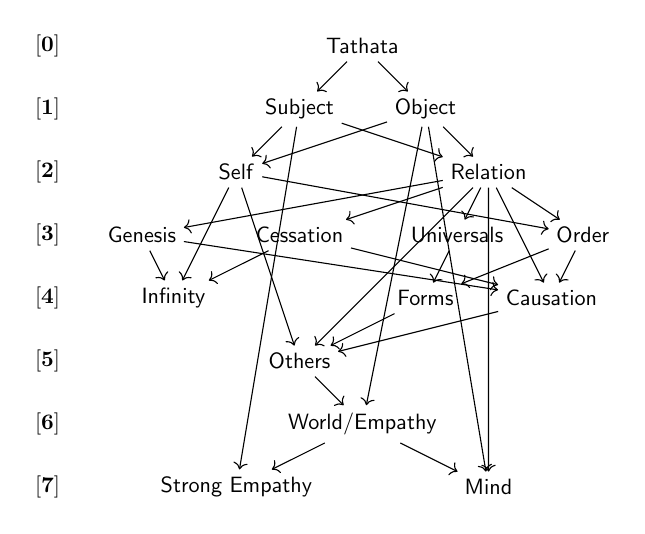
\begin{tikzpicture}[scale=0.80,transform shape]
	\node (pp0) at (-5, 0) {[\textbf{0}]};
	\node (pp1) at (-5, -1) {[\textbf{1}]};
	\node (pp2) at (-5, -2) {[\textbf{2}]};
	\node (pp3) at (-5, -3) {[\textbf{3}]};
	\node (pp4) at (-5, -4) {[\textbf{4}]};
	\node (pp5) at (-5, -5) {[\textbf{5}]};
	\node (pp6) at (-5, -6) {[\textbf{6}]};
	\node (pp7) at (-5, -7) {[\textbf{7}]};

	\node (p0) at (0, 0) {\textsf{Tathata}};
	\node (p1a) at (-1, -1) {\textsf{Subject}};
	\node (p1b) at (1,-1) {\textsf{Object}};
	\node (p2a) at (-2,-2) {\textsf{Self}};
	\node (p2b) at (2,-2) {\textsf{Relation}};
	\node (p3a) at (-3.5,-3) {\textsf{Genesis}};
	\node (p3b) at (-1,-3) {\textsf{Cessation}};
	\node (p3c) at (1.5,-3) {\textsf{Universals}};
	\node (p3d) at (3.5,-3) {\textsf{Order}};
	\node (p4a) at (-3,-4) {\textsf{Infinity}};
	\node (p4b) at (1,-4) {\textsf{Forms}};
	\node (p4c) at (3,-4) {\textsf{Causation}};
	\node (p5) at (-1,-5) {\textsf{Others}};
	\node (p6) at (0,-6) {\textsf{World/Empathy}};
	\node (p7a) at (-2,-7) {\textsf{Strong Empathy}};
	\node (p7b) at (2,-7) {\textsf{Mind}};

	\begin{scope}[every path/.style={->}]
		\draw (p0) -- (p1a);
		\draw (p0) -- (p1b);
		\draw (p1a) -- (p2a);
		\draw (p1a) -- (p2b);
		\draw (p1b) -- (p2a);
		\draw (p1b) -- (p2b);
		\draw (p2b) -- (p3a);
		\draw (p2b) -- (p3b);
		\draw (p2a) -- (p4a);
		\draw (p2a) -- (p3d);
		\draw (p2b) -- (p4c);
		\draw (p2a) -- (p5);
		\draw (p2b) -- (p5);
		\draw (p3a) -- (p4a);
		\draw (p3b) -- (p4a);
		\draw (p4c) -- (p5);
		\draw (p5) -- (p6);
		\draw (p1b) -- (p6);
		\draw (p6) -- (p7a);
		\draw (p6) -- (p7b);
		\draw (p1a) -- (p7a);
		\draw (p1b) -- (p7b);
		\draw (p2b) -- (p7b);
		\draw (p2b) -- (p3c);
		\draw (p2b) -- (p3d);
		\draw (p3c) -- (p4b);
		\draw (p3d) -- (p4b);
		\draw (p3a) -- (p4c);
		\draw (p3b) -- (p4c);
		\draw (p3d) -- (p4c);
		\draw (p4b) -- (p5);
	\end{scope}
\end{tikzpicture}
\caption{\label{fig:axiomtree}Epistemic Priority}
\end{figure}

Epistemic priority is useful in that it allows us to think precisely about precedence of ideas. In particular, it provides a firm basis for our earlier suggestion that consciousness need not be justified in relation to a presupposed brain, since the latter occurs arguably at a lower epistemic priority, and certainly not at a higher one. Also significantly, it may be seen that ``empirical'' (i.e. our dialectical) scientific method operates at epistemic priorities $\geq 3$ (and $\geq 6$ if we require it to conform to traditional dialectical agreement), while dhyana as a direct investigation of consciousness proceeds at priorities $0 - 1$ (while also reducing to $\geq 6$ if results are communicated dialectically). This does not speak to \emph{validity} in any sense -- it only provides criteria by which different types of knowledge may be related. It may be possible for lower priority knowledge to be justified in terms of higher priority knowledge, but the reverse endeavor is not well-founded.

\subsection{Additional Notes}

The following are uncategorized, inchoate notes of a philosophical nature that are recorded here as they may be found to be clarifying.

\paragraph{The Ultimate Primitive} \label{sec:ultpri} Plato conceived that the world of the senses is subsidiary to a more pure reality of `the forms.' He imagined that particular things perceived by the senses (e.g. a particular cat) are imperfect approximations of the pure, unique, eternal forms (e.g. an ideal cat), and that these forms alone are truly real. We may consider Plato's forms to typify a conception of an ultimate primitive in terms of specification of \emph{inherent nature}.

Another conception of an ultimate primitive is one of pure causation, perhaps most developed in some strands of early buddhism which conceived all reality to be in flux, an eternal stream of ``becoming,'' with no well-defined persistent entities. Thus this ultimate primitive is purely \emph{functional}.

A third conception of an ultimate primitive is the notion of `dharmas' as used especially in Mahayana Buddhism. Dharma is notorious for being a very difficult word to translate. A common, general difficulty encountered in translation is when no exact equivalent exists in the target language, but in the case of dharma, in addition to this difficulty, it seems likely that the word encodes one of those ``radically general'' concepts mentioned earlier that are hallmark of buddhist philosophy. This would account for the fact that dharma is used in a wide variety of different contexts; uses which are difficult to reconcile in terms of particulars if one is not aware of the underlying general notion. Based on usage and on discussion of this issue (e.g. in \cite{dharmadhatu}), it seems plausible that dharma refers to ``essential principle'' or ``underlying pattern'' in a very general sense. Thus we may speak of the dharma of a scorpion, or the dharma of human society, or the dharma of a warrior. That is, a scorpion, human society, and a warrior as corresponding to ``patterns'' in reality\footnote{It seems to be the case that dharma over time may have taken on a ``Platonic'' flavor in common usage, referring not merely to the abstract pattern of, say, a warrior, in reality, but more specifically, that pattern corresponding to the \emph{ideal} warrior, or more generally the pattern corresponding to the ideal -- and unspeakable -- version of oneself.}.

Another way of looking at this is that in thinking about specific physical objects, a convenient abstraction that unifies them is `thing'. But when we talk of ideas, or of feelings and thoughts, or of collections of substantial objects, it becomes less apt to think of them as things. `Dharma' seems to be the abstraction we are reaching for here which applies to anything conceivable. Additionally, while `thing' has the effect of ``forgetting'' all specific information about an entity, `dharma' instead (as envisioned here) operates in two modes: the first may be framed as saying that an entity ``is'' a dharma; that is, acknowledging an (any) entity as being a pattern in reality, in the same manner that `thing' does. The second mode is to refer specifically to the entity itself -- without excluding any specific details but not identifying any either -- as it exists as a pattern in reality; ``the dharma that is this entity'' or ``the dharma \emph{of} this entity.'' The dharmas thus can be taken to exist in a one-to-one correspondence with elements of reality. In this elaboration it appears to emerge that `thing' has a different orientation than `dharma': the former is an abstraction deriving from convenience, while the latter derives from and embodies a particular philosophical outlook. Note that this conception of dharma exists at epistemic priority \textbf{0} as it entails neither subject nor object nor any assumptions as to the nature of the thing being discussed. This interpretation of `dharma' seems to be supported in that an alternate name for `tathata' appears to be `dharmata.' Dharmas thus can be viewed as a particular type of ultimate primitive, of a particularly \emph{elemental} sort.

Identities provide yet another conception of an ultimate primitive, which can be seen to exhibit qualities of both the `forms' and `functional' primitives. Identities are like the forms in that they apply to the nature of things as entities in themselves. At the same time, consistent with the buddhist idampratyayata, the properties of an identity are \emph{context-dependent} and not absolute. An ideal bed only exists in relation to an implicit anonymous identity with respect to which the \emph{action} of the identity conforms to `bed-ness.' An identity and its action are mutually defining and not independent, and these may differ from context to context. Additionally, the action of the identity conveys structural information ``functionally'' and thus provides a mechanism for causation. Indeed ``properties'' of an identity derive from causal effects on the identities with respect to which those properties are defined. This qualifies the relationship of identities to form and function, but not to dharmas. With dharmas, we could consider that identities provide a \emph{model} for the more elemental notion of dharmas. This also suggests a general principle: that a model for $X$ always exists at a strictly lower priority than $X$.

Summarizing, we may say that the dharmas are the unspeakable, elemental reality underlying particular things; and forms, causation, and identity architecture are conceptions of, models for the dharmas.

\paragraph{`Seamlessness' of Identity Architecture} Identity is a proposed formal model for the notion of a generalized `thing'. As a result, it applies universally. The upshot of this is that a development in a particular area can be translated into a development about identities more generally, which can once again be translated into a development in a different, ``unrelated'' domain. Insights in one field could translate into insights in all fields, and vice versa, via the translation into identities. For instance, the mechanics of evolution by natural selection in biological systems may be abstracted as a causal interaction in a bodhitree, and any results found for this bodhitree would apply to any other field where (and to the extent that) the dynamics can be reduced to a bodhitree that is topologically similar to the one derived for biological systems. This notion likely has a precise category-theoretic formulation, involving free and forgetful functors and so on, which may be developed in future work.

\paragraph{On Universals} \label{sec:onuni} There seem to be two qualitative entities characterizable as ancestors in a bodhitree. First, there are causal ancestors. That is, identities that, through interactions with other identities, \emph{cause} the genesis of other identities which are its descendants. The second kind correspond to the notion of `universals' in philosophy; that is, general notions of which particular things are specific instances. For example, mangoes, lemons, and tomatoes exist in the world, but the abstract notion of a `fruit' does not, even though all mangoes, lemons, and tomatoes are conceived to be instances of it. Philosophers since ancient times have wondered about the epistemic status of the universals -- where do they exist? What is their nature? We could conceive `fruit' as corresponding to an identity which is an ancestor of particular, ``real,'' fruits encountered in the world. Now, if the particular fruits exist in the world context, which context does `fruit' exist in? A possible answer is that both `fruit' as well as the definability of such a bodhitree exist in the (any) mind context associated with the world, rather than in the world itself, following from an Axiom of Worlds intuition coupled with the evident fact that human minds are, in fact, able to conceive of an abstract fruit though such a conception does not exist in the world. This conception motivates the generalization that in any context treated as a world, universals in relation to that context exist in minds in that world, and universals in relation to those minds exist in minds within those minds. This conception also suggests that the dichotomy between ``causal'' and ``universal'' ancestors derives from the former existing in the world, and the latter existing in the mind, and suggesting further that universals may participate in causal interaction in the mind, which seems to be true\footnote{Identity ancestors ``acting through'' descendants in the manner that people act through organizations (as described in \autoref{sec:topstr}) does not obviously fit either universals acting through particulars or causal ancestors acting through effects. Further refinement in the mathematical models will likely reveal the exact conception of and relationship between these types of entities.}.

\paragraph{The `Acts-through' relationship} As discussed above philosophy has traditionally been interested in the relationship between particular things and `universal' properties which they may share. The object-oriented paradigm in computer programming may be viewed as a recent exploration along these lines. In this paradigm, for modeling purposes, a distinction is made between the relationships `is-a' and `has-a'. We may consider an `acts-through' relationship as possibly being more clarifying as a general conception. That is, while a square `is-a' rectangle, no one would say that an orchestra `is-a' human being. And yet, with identities the important consideration seems to be whether an identity can \emph{act as} another identity or not (this is essentially the idea of `polymorphism' in object-oriented programming). In this example, if a human being is needed for some purpose, one may just as well use an orchestra since an orchestra can do anything that a generic human being could. But the reverse is not true, if an orchestra is needed, a human being could not serve that role. The relationship here is that the human being `acts through' the orchestra. Similarly, a rectangle `acts through' a square. This relationship is expressed as an ancestor `acting through' a descendant in a bodhitree\footnote{Ancestors `acting through' descendants is equivalently framed as descendants `acting as' ancestors, but the former provides some clarity on economic considerations of fairness developed in \autoref{sec:humins}.}, subject to any mathematical constraints or modifications imposed by the model.

\paragraph{Bodhitree-aware Nomenclature} In naming things, it may be useful to have conventions as to whether the name describes the thing itself, or its lineage. For example, in talking about Plato's philosophy, we might say ``Platonic,'' while in talking about philosophy derived from, influenced by, or in the style of Plato we might say ``Platonian.'' It may be impractical to impose such conventions over the current diversity (and inconsistency) in suffix usage, so perhaps some alternate system (e.g. involving hyphens) should be developed. This would also alleviate the great confusion that arises from present terms such as the ``Western philosophy'' and ``Indian philosophy'' already employed above, which suggest that the salient constituents in philosophy are geographical (or worse, national) in nature. Instead, the terms ought to represent their lineage; perhaps ``Parmenidean''\footnote{from Parmenides, a founding figure in ``Western'' philosophy.} and ``Upanishadian''\footnote{from the Upanishads, foundational philosophical works in the ``Indian'' tradition.} philosophy would be better. It is likely that a \emph{common ancestor} is the most appropriate basis in naming things. Similarly terms like ``English mathematics'' and ``German philosophy'' should be avoided in favor of terms indicating lineage or substance. Other instances of confusion (usually unconscious confusion) arise in terms describing things existing at different times, where a modern name is retrospectively applied to an ancestral thing. As a didactic example, ``ancient China'' is particularly undesirable, applying not only the name of a modern identity to an ancient one, but additionally one that, being predominantly associated with a modern nation largely deriving from modern political ideas (such as those of Marx, Lenin and Mao) and less so derivative of the traditions of the ancient identity under consideration, is a misleading characterization of the ancient ancestor masquerading as ``China.'' Thus the nation of the People's Republic of China is an entirely different identity from the various cultural identities that are significantly associated with (but not significantly derivative of) that geographical region of the world, and which do actually derive significantly from the ancient traditions under consideration. Likewise, ``ancient Greece,'' ``ancient Egypt'' should be avoided in favor of something like ``X ancient civilization (associated with region Y),'' where `X' is bodhitree-derived if necessary and Y is the associated geographical region that may be included if warranted. Instances of fallacious national association in nomenclature particularly abound, and should be avoided. As another example, ``Western civilization'' and ``Eastern civilization'' are, in addition to falling prey to fallacious geographical association, also undesirable in another respect, which is that due to the nonlinear, recursive nature of identity interactions, the development of civilization around the world cannot be considered in the isolated manner that these terms presuppose. Such oversimplifying terms may also be avoided by employing more precise bodhitree-aware conventions such as the suggested common-ancestor (i.e. anonymous) convention. This would enable the study of cultural evolution \emph{structurally} as identity trees, rather than geographically or by any other such incidental -- even if salient -- attribute.

\section{Interpretation} \label{sec:interpretation}

As suggested earlier, identity can be seen as the substance of our reality. By its status in this regard, the models presented above allow us to reinterpret common ideas and institutions.

\subsection{Currency} \label{sec:currency}

A single organism (such as a human) must feed itself, defend itself against predators and competition, and must have access to a safe location for resting. When such organisms band together into larger groups, economies of scale emerge enabling the division of responsibilities into focused functional groups, which allows the requirements of all members to be aggregated and handled in batches. The group can be said to comprise a higher organism, i.e. a hive identity. As the organism grows in scale, it becomes more challenging to properly assess its needs, and so a market economy emerges where these needs can be determined organically: a shortage of a particular resource drives up the incentive to address it within the organism, and when that incentive exceeds the opportunity cost for some subset of members to address it, that subset rises to the need.

Initially, the organism may sustain a barter economy, but over time, trade in specific goods and services becomes cumbersome and it becomes apparent that the objective of the implicit market economy is to accord -- \textit{within the mind context} -- a level of access to goods and services to a constituent that is commensurate with the value of the goods and services provided by it. It is soon realized that this may be more precisely captured in a form of monetary currency.

When the organism encounters other human settlements in the world, a form of currency exchange is developed that allows trade between them. We can say that the value possessed by a constituent represents a fraction of the total value in the \textit{mind}, which is convertible into a fraction of total value in the \textit{world}, and so on, in a self-similar manner. This fraction is naturally characterized as a real number between $0$ and $1$, which we can define as representing the extent to which the \textit{agency} of the hive is expressed in that constituent. We may equivalently conceive of this as the \textit{wealth} of the constituent in the context. This notion is related to today's notion of (financial) ``wealth,'' motivating the choice of terminology, but it is important to note that they have a different conceptual basis, and we can consider the latter to be a crude approximation (``crude'' for reasons which will be explored in \autoref{sec:humins}) of the conception as defined here.

Observe further that under this characterization, the fraction of context value contained in a constituent $q_i$ can be interpreted as the proportion of the ``amount'' of identity of $Q$ that is contained in $q_{i}$, since $q_{i}$ ``controls'' the functioning of $Q$ in the world precisely to the extent of its own wealth within the mind $\mathcal{M}$ of $Q$. And in the same manner, $Q$ guides the functioning of the world identity to an extent commensurate with its wealth in the context $\mathcal{W}$, and so on. In this sense, since all constituents in a context derive from the anonymous identity of that context, we can equate the totality of wealth in a mind with the anonymous identity of the mind (i.e. $1.0 \varnothing_Q$), which in turn we may as well equate with the identity itself as it exists in the world (i.e. $1.0 \varnothing_Q = w_{\mathcal{W}}(Q) \varnothing_{\mathcal{W}}$).

\begin{defn}[Wealth]
	In any context $\mathcal{W}$, \emph{wealth} is a function defined on $\mathcal{W}$ that maps each constituent $q \in \mathcal{W}$ to a real number $w_{\mathcal{W}}(q) \in [0, 1]$ at a particular point in time, and is recursively determined as:
	\begin{equation} \label{eq:wealth}
		\begin{split}
			w_{\mathcal{W}}(\varnothing_{\mathcal{W}}) &= 1.0 \\
			w_{\mathcal{W}}(q) &= \sum_{i} w_{Q_i}(q) \cdot w_{\mathcal{W}}(Q_i) ;
		\end{split}
	\end{equation}

	where the $Q_{i}$ correspond to minds in $\mathcal{W}$ to which $q$ belongs, and $w_{x}$ represents wealth in context $x$\footnote{While the wealth of the anonymous identity being defined as $1.0$ provides a ``base case'' for the definition, the characterization of wealth in terms of constituent minds is inductive in the ``wrong direction,'' although still presumably valid. A correct recursive definition is left for future work, and will likely involve the proportion of an abstraction of time that the anonymous identity spends as each non-anonymous descendant.}.
\end{defn}

Thus, in this conception, currency can be seen as a manifestation within the systems of human society of anonymous identity. This can be empathized with when one considers that every dollar (or whatever unit of currency) is equivalent to every other dollar and devoid of identity without reference to its context (would you accept a form of currency without knowing which country it's from?), and in sufficient quantities can ``take the form'' of any identity in the context in a process we call ``purchasing.'' Money can enable any individual or enterprise, regardless of form or purpose, and so it too is ``like water.''

Now with money proposed as corresponding to ``quantity'' of anonymous identity, we observe further that maintaining discrete quantities of currency within constituents for any nonzero extent of time is inefficient. Learned wisdom has it that one must keep money ``moving,'' but this notion isn't captured formally within our economic systems. It could be useful if such a continuous, time-variant system of currency were adopted, where all transactions occur as rates and times and not necessarily as discrete quantities. We could call such a quantity the \textit{influence} of an identity in a context.

\begin{defn}[Influence]
	For identities $q, r \in \mathcal{W}$, an \emph{influence} applied by $q$ on $r$ is a function $n(t)$ such that:
	\begin{equation}
		\begin{split}
			\Delta w(r) &= \! \int_{0}^{T} n(t)\,dt \label{eq:influence}, \text{ and} \\
			\Delta w(q) &= - \Delta w(r) ;
		\end{split}
	\end{equation}

	where $n$ is the influence applied on $r$ by $q$, $\Delta w$ is the change in wealth of an identity, and $T$ is the duration for which the influence is applied. An edge in a bodhitree can be interpreted to entail such an influence.

\end{defn}

Note that a one-time discrete exchange of money would be a special case of the above, and can be captured by employing an impulse function as the influence. In general the influences into and out of an identity should be at a steady state, i.e. their sum should equal zero:

\begin{equation}
	\sum_{i} n_i(t) = 0 .
\end{equation}

Influence and wealth are developed further in the section on \hyperref[sec:humins]{Human Institutions}.

\subsection{Identity and the Brain} \label{sec:idebra}

The natural application of the identity model is, of course, to the brain. Before we continue, it is worthwhile to reaffirm that our experience of the physical world exists entirely within a mental representation of that world which, we proffer, is in terms of identities. Within this representation, actions that we take actually manifest in the physical world, and interactions that occur in the physical world occur also in this representation. In other words this representation in the mind is in a state of persistent equivalence with the physical world, which we identified earlier as a form of categorical equivalence or adjunction. We will generally avoid speaking directly of this equivalence between actions in the mind and actions in the physical world, and will make no distinction between them. Its existence, however, has important implications which we address in the section on \hyperref[sec:natphe]{natural phenomena}.

\subsubsection{The Self} \label{sec:theself}

Anything we can conceive of as a thing is an identity in the sense of this document. Clearly a person meets this requirement and is an identity. Following from the definition of identity, the person defines a mind context relative to the world, which can be seen to correspond to the traditional idea of a mind (of course the terminology was chosen for this reason). By \autoref{lem:maya}, all things in the world have a representation in the mind as thoughts (a claim supported by our ability to think about objects even when we close our eyes). Now as a person, one is able to conceive of oneself, and is able to act as a causative agent in the form of this ``self.'' The conception of the self can be seen to derive also from \autoref{lem:maya}: since every thing is represented in the mind as a thought, the identity itself, being a thing in the world, must exist in the mind as a thought, or a representation of itself. This natural characterization is shown in Fig.~\ref{fig:self}, and corresponds to the notion of the ``self.''\footnote{This conception of self is in the literal sense of ``self-reference'' rather than that of ``ego.''}

\begin{figure}[htp]
	\centering
	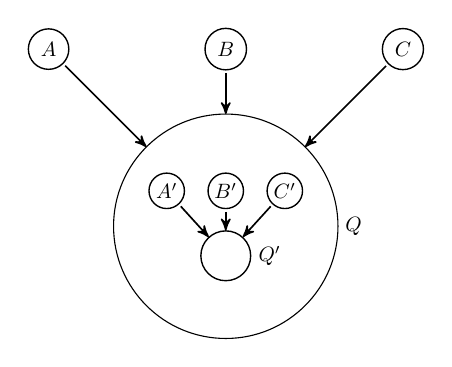
\begin{tikzpicture}[scale=0.75,transform shape]
		%\tikzstyle{LabelStyle}=[fill=white,sloped]
		%\draw[solid] (0,0) circle (2cm);
		\GraphInit[vstyle=Normal]
		\Vertex[x=-3,y=3,L=$A$]{A}
		\Vertex[x=0,y=3,L=$B$]{B}
		\Vertex[x=3,y=3,L=$C$]{C}
		{
			\tikzset{VertexStyle/.style = {draw=black,shape=circle,minimum size=3.8cm,inner sep=0pt}}
			%\SetVertexNoLabel
			\Vertex[x=0,y=0,L=$Q$,LabelOut=true]{Q}
		}
		%\tikzset{VertexStyle/.append style = {draw=darkgray,text=darkgray}}
		{
			\tikzset{VertexStyle/.append style = {shape=circle,minimum size=0.6cm,inner sep=0pt}}
			\Vertex[x=-1,y=0.6,L=$A'$]{A'}
			\Vertex[x=0,y=0.6,L=$B'$]{B'}
			\Vertex[x=1,y=0.6,L=$C'$]{C'}
		}
		{
			\tikzset{VertexStyle/.append style = {shape=circle,minimum size=24pt,inner sep=0pt}}
			%\SetVertexNoLabel
			\Vertex[x=0,y=-0.5,L=$Q'$,LabelOut=true]{Q'}
		}
		\tikzstyle{EdgeStyle}=[post]
		\Edge[](A)(Q)
		\Edge[](B)(Q)
		\Edge[](C)(Q)
		%\tikzset{EdgeStyle/.append style = {draw=darkgray,text=darkgray}}
		\Edge[](A')(Q')
		\Edge[](B')(Q')
		\Edge[](C')(Q')
	\end{tikzpicture}
	\caption{\label{fig:self}The Self}
\end{figure}

\begin{defn}[Self]
	Given an identity $Q = (\mathcal{M}, B, \phi, \mu, \omega)$ in a world $(\mathcal{W}, \psi)$, the \emph{self} of $Q$ is defined to be the thought $Q' = (\mathcal{M}', B', \phi', \mu', \omega')$ within $\mathcal{M}$ such that $Q' = \mu(Q)$.
\end{defn}

Note that as all identities are qualitatively equivalent, in particular $Q'$ is as fully an identity as $Q$, and can sustain a representation of itself within it. Similarly, the identities $A'$, $B'$, and $C'$ are representations of $A$, $B$ and $C$ within $Q$, and can harbor representations of each other within themselves within $Q$, and so on. Furthermore, each constituent in the mind of $Q$ can represent also the self of $Q$, i.e. can conceive of $Q'$ -- this fractal nature can be experienced when we think about doing something, for example, and then think about thinking about doing that thing (in Fig.~\ref{fig:self}, this would be experienced as the self of the thought (e.g. $A'$) that is thinking about the action of the self (i.e. $Q'$) of $Q$). This is exactly the kind of self-recursive nature described by Hofstadter\cite{geb}, corresponding approximately to what he refers to as a ``strange loop.''\footnote{The correspondence to Hofstadter's conception would probably be more exact in a non-well-founded (in the sense of set theory) specification.}

Further, it appears that when we think of anything, we ``are'' the self of that thought. Thinking of a book in one's field of view is experience as the self of that book-as-a-thought. Thinking of the self, we are the self of the self.

\subsubsection{Language} \label{sec:language}

Linguistic communication structurally can be seen as an instance of a more general process of conveyance of identity trees from one mind to another by use of dialectically constructed isomorphisms. Identities corresponding to `words' represent these dialectically constructed isomorphisms for language in particular; that is, words are intended to be isomorphic across minds. Although in practice they may not be so, we reinforce this by having universally-agreed-upon lexicons such as dictionaries and encyclopedias for arbitration of any disagreements\footnote{which reinforce isomorphism by the transitivity of the relation of being isomorphic.}.

Spoken language (for example) can be characterized as an action of the identities in the mind on identities in the world (which includes our physical forms and in particular our vocal cords), followed by, from the perspective of the other person, an action of the world (including their physical forms and in particular their auditory structures) on the identities in their mind. This would be facilitated at either end by an expression and a perception functor, respectively. Under this description, the ``deep structure'' described by Chomsky\cite{chomsky} could be taken to correspond to the identity architecture of the mind, some subset of which is isomorphic to the linguistic expression in each mind. This entire preceding interaction would be represented in the minds of the participants as existing within a nested mind constituted by (representations of) the two participants in the conversation. In the mind of one of the participants, this identity may communicate ``linguistically'' with other identities in his mind, ``spreading the word,'' as it were. Over time, the information gleaned in the conversation could thus be incorporated into the identity structure of the mind as a whole, with any remaining particulars being recalled from this identity as needed. This ``social'' nature of the identities in the mind is reminiscent of Minsky's ``society of mind,''\cite{minsky} where he considers specialized ``agents'' in the mind that work together in hierarchies to accomplish complex tasks. This process can also be considered an instance of the general recursive process of `cognition' outlined in the following section.

Sentences can be taken to represent ordered subsets of words which serve to construct and communicate identities that are not part of the standard lexicon (or else we would just use the word corresponding to the intended communication). The reason we resort to sentences instead of simply extending our lexicon to contain any novel identities is that if indeed ``subsets of words'' are what it takes to capture our experience, then representing new ideas directly as identities would require that each person carry around a representation of $2^{Card(W)}$\footnote{In fact, as mentioned previously, sentences are \textit{ordered} subsets and not just subsets. But since the order can be varied under alternate grammatical constructions (e.g. ``The girl threw the ball'' vs. ``The ball was thrown by the girl''), we consider the weaker model of unordered subsets of words as it is sufficient to express the argument. The number of (unordered) subsets of a set of size $n$ is $2^{n}$, which is strictly greater than $n, \forall n$.} words in their minds (with the attendant necessity of achieving dialectical isomorphism for each of them), where $W$ is the set of words they would have to know if they used sentences instead. This also implies that with a countably infinite number of words, we can represent an uncountable number of ideas using sentences, and therefore it is a superior computational model regardless of any efficiency considerations of storing additional words in one's head.

As such, sentences represent computational instructions to construct new identities from available ones. As an example, we can envision in a typical sentence each word and in particular the nouns as corresponding to identities in the shared lexicon; adjectives as conveying heredity of an identity that is not part of the lexicon -- and therefore enabling the recipient to construct this identity in their mind; verbs as conveying actions of identities on other identities and therefore communicating the genesis of new identities, which is simulated in the mind of the listener.

\subsubsection{Cognition} \label{sec:cognition}

When an experience in the physical world $\mathcal{W}$ is apprehended by a person $p = (\mathcal{M}_{p}, \phi) \in \mathcal{W}$, it can be seen to be an action of identities in the representation (via the perception functor) of the world in the mind, on the self. This action translates in the mind of the self into actions on the identities -- that is, the thoughts -- of the self. This further translates into actions on the selves of the thoughts of the self, and so on (since we can be considered to embody a particular (single) self at any point in time, it's possible that a particular computation is prioritized when we embody a self affected by it. This could represent the nature of the interactions that are described below in \hyperref[sec:dreams]{Dreams}). Each action gives rise to a reaction and to genesis, and these are all aggregated outward to form the reaction of the self in the mind, which, via the expression functor, translates into the reaction of the person to the experience in the physical world. The nature of this aggregation remains to be specified in future work, but may possibly be modeled in terms of the extent to which the identity of $p$ (in the sense of anonymous identity, i.e. ``quantity'' or wealth) is expressed in each of its constituent thoughts. All thoughts in the self, and thoughts within the minds within the self, can be conceived to weigh in on each issue in terms of their reactions to it, and be considered to the extent of their influence in the relevant contexts. This is developed further in the section on \hyperref[sec:humins]{Human Institutions}.

Beyond representation of the physical architecture of the world, our minds also represent identities such as human motivations and communications that are present in minds within the physical world (note that communications exist not within a human mind but in the mind of the hive identity constituted by participants in the communication. These participants form the body of this hive identity) that do not themselves have a faithful or persistent physical representation. We can understand this representation as existing in minds within our mind that are representations of those minds in the physical world. That we are able to construct these representations derives from the partial order defined by bodhitree evolution; that is, since new identities in a context manifest via actions of existing identities in the context, evolution of a context cannot simply occur arbitrarily within all possibilities supported in the universe. When an identity in the world is considered, therefore, we are able to inductively determine a heredity based on other known and inferred identities in the world and in minds within the world. In particular, every identity in the world has a defined heredity in the mind, even if this is simply that that identity is anonymous (i.e. descended directly from the unique anonymous identity of the world).

Edges in a bodhitree as discussed earlier can be interpreted as entailing influence, and as such, heredity construction could include assignment of likely influence of each inferred ancestor. Since influence is in terms of fractions of a particular anonymous identity and therefore takes values between $0$ and $1$, this could naturally correspond to an interpretation as probabilities, and it's possible a Bayesian or other probabilistic model could inform this process of heredity construction. In general in probability theory, the likely occurrence of any event has an associated distribution, which itself has an associated ``confidence'' distribution, which in its turn can also have a confidence distribution, and so on. These nested confidence distributions appear to correspond to models as nested selves.

Toward motivating future development, these considerations may be taken to suggest that cognition, in the sense of understanding, reasoning, and reacting, is likely best characterized as a recursive ``algorithm'' that is applied once at each mind/world interface, and whose result is incorporated in repeated applications of the same process within nested minds. As such it would be closely related to the mechanism of genesis, and it seems likely that a simple principle can be distilled here that would subsume both notions.

\subsubsection{Awareness and Memory} \label{sec:awamem}

By the definition of identity, the mind is a persistent representation of the world and every thing in the world is present in the mind to the extent that it is apprehended. Now we examine \autoref{lem:maya} to derive yet another noteworthy implication. Since representations of things exist in minds but thoughts don't exist in worlds, the lemma also implies that any identity $q$ within a world $\mathcal{W}$ contains a full internal representation of every mind to which it belongs\footnote{This follows from the fact that $q$ transitively corresponds to a thought in the mind of each of its descendants. Note that the mind of $q$ thus satisfies the ``Axiom of Worlds'' in relation to each of those descendant minds, and may represent any identity that could be conceived from the constituents of those minds.}. That is, if $q$ constitutes $n$ things in $\mathcal{W}$, then each of those $n$ minds are represented in $q$, although of course no representation of those minds necessarily exists in $\mathcal{W}$. As an illustration, in Fig.~\ref{fig:awareness}, the entire figure is also present within $B$. Taken together with the ``strange loop'' pattern of self manifestation discussed in \autoref{sec:theself} above, this aspect is highly reminiscent of the buddhist doctrine of ``interpenetration'' of all reality, as embodied in the vivid account of ``Indra's Net.''\cite{avatamsaka}

\begin{figure}[htp]
	\centering
	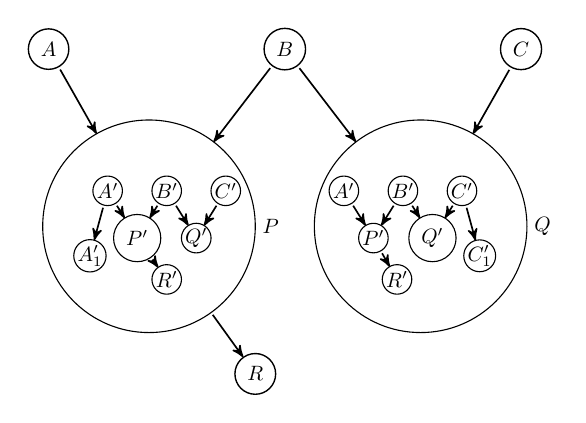
\begin{tikzpicture}[scale=0.75,transform shape]
		%\tikzstyle{LabelStyle}=[fill=white,sloped]
		%\draw[solid] (0,0) circle (2cm);
		\GraphInit[vstyle=Normal]
		\Vertex[x=-4,y=3,L=$A$]{A}
		\Vertex[x=0,y=3,L=$B$]{B}
		\Vertex[x=4,y=3,L=$C$]{C}
		{
			\tikzset{VertexStyle/.style = {draw=black,shape=circle,minimum size=3.6cm,inner sep=0pt}}
			\Vertex[x=-2.3,y=0,L=$P$,LabelOut=true]{P}
			\Vertex[x=2.3,y=0,L=$Q$,LabelOut=true]{Q}
		}
		\Vertex[x=-0.5,y=-2.5,L=$R$]{R}
		{
			\tikzset{VertexStyle/.style = {draw=black,shape=circle,minimum size=0.5cm,inner sep=0pt}}
			% mind of P
			\Vertex[x=-3,y=0.6,L=$A'$]{A'}
			\Vertex[x=-2,y=0.6,L=$B'$]{B'}
			\Vertex[x=-1,y=0.6,L=$C'$]{C`}
			\Vertex[x=-3.3,y=-0.5,L=$A_{1}'$]{A"}
			\Vertex[x=-1.5,y=-0.2,L=$Q'$]{Q`}
			\Vertex[x=-2,y=-0.9,L=$R'$]{R'}
			% mind of Q
			\Vertex[x=1,y=0.6,L=$A'$]{A`}
			\Vertex[x=3,y=0.6,L=$C'$]{C'}
			\Vertex[x=2,y=0.6,L=$B'$]{B`}
			\Vertex[x=1.5,y=-0.2,L=$P'$]{P`}
			\Vertex[x=3.3,y=-0.5,L=$C_{1}'$]{C"}
			\Vertex[x=1.9,y=-0.9,L=$R'$]{R`}
			% selves
			\tikzset{VertexStyle/.style = {draw=black,shape=circle,minimum size=0.8cm,inner sep=0pt}}
			\Vertex[x=2.5,y=-0.2,L=$Q'$]{Q'}
			\Vertex[x=-2.5,y=-0.2,L=$P'$]{P'}
		}
		%\tikzset{VertexStyle/.append style = {draw=darkgray,text=darkgray}}
%		{
%			\tikzset{VertexStyle/.append style = {shape=circle,minimum size=24pt,inner sep=0pt}}
%			%\SetVertexNoLabel
%			\Vertex[x=0,y=-0.5,L=$Q'$,LabelOut=true]{Q'}
%		}
		\tikzstyle{EdgeStyle}=[post]
		% world
		\Edge[](A)(P)
		\Edge[](B)(P)
		\Edge[](B)(Q)
		\Edge[](C)(Q)
		\Edge[](P)(R)
		%\tikzset{EdgeStyle/.append style = {draw=darkgray,text=darkgray}}
		% mind of P
		\Edge[](A')(P')
		\Edge[](B')(P')
		\Edge[](A')(A")
		\Edge[](B')(Q`)
		\Edge[](C`)(Q`)
		\Edge[](P')(R')
		% mind of Q
		\Edge[](A`)(P`)
		\Edge[](B`)(P`)
		\Edge[](B`)(Q')
		\Edge[](C')(Q')
		\Edge[](C')(C")
		%\Edge[](B`)(B")
		\Edge[](P`)(R`)
	\end{tikzpicture}
	\caption{\label{fig:awareness}Interpenetration/``Awareness''}
\end{figure}

While this representation in $B$ does not directly include any thoughts within the minds of $A$ or $C$ that are not expressed in the worlds $P$ and $Q$, such thoughts may be inferred inductively via the mechanism of cognition. Like any other identities in this representation, these represented thoughts are not guaranteed to be isomorphic to those they represent, but are likely to have a structural relationship to them that is to be specified in future work\footnote{The Advaita conception of maya suggests that the mental representation is partial (due to \textit{avidy\={a}} or, loosely, ``ignorance'') and entails ``projections'' of a known particular thing in place of an unseen particular instance of a perceived general thing, as illustrated in the metaphor of the rope and the snake\cite{waite}. This seems a plausible characterization in relation to the perception functor. As an aside, a related (possibly ancestral) idea in this connection is the buddhist \emph{trisvabh\={a}va}: that for any thing there are ``Three Natures'': (1) a superficial nature or appearance, (2) a structural nature consistent with that appearance, and (3) an underlying ``true'' nature consistent with that structure\cite{trisvabhava}. Interestingly enough, if these interpretations are accurate, Plato's Allegory of the Cave may equivalently serve to illustrate these ideas: the taking of the shadows to be ``real'' is the superficial nature, the shadows themselves and their interplay are the structural/``contingent'' nature, and the reality casting the shadows is the ``true'' nature. Conjecturally, it's possible Plato's Allegory made it in some form to the Indian Subcontinent and, in combination with the buddhist penchant for what can be described as ``radical generality,'' motivated the general principle that is trisvabhava, which later informed the more nuanced Advaita conception (which, incorporating as it does the ideas of universals and particulars, may reflect additional influence of the ``Greek'' tradition). To investigate such possibilities, a characterization of the ``fidelity'' of information transfer in the world (e.g. in terms of characteristic time and distance) across eras would be useful in framing theories of historical civilizational interaction and the evolution of ideas in a nonlinear world.}. This persistent internal representation of myriad worlds, together with the recursive representation of the self described previously, can be seen to constitute the structure of our experience of conscious awareness, and, in the aggregate, ``life.''

Memory, specifically the process of ``recollecting'' something, can be characterized as the act of utilizing available information to assemble the heredity of the mind within which the desired information exists, and then simply deriving a world-representation (via successive expression functors) of the identity corresponding to the memory. This world-representation would include any modifications or retractions imposed by the contexts along the path to the world.

\subsubsection{Dreams} \label{sec:dreams}

Every night of every day, every person in the world sleeps. And dreams. We've been doing this for thousands, millions of years. But the explanation of the nature of dreams has largely eluded us. Sometimes we wake from one and the recollection of it quickly escapes description. The dream is on the tip of one's tongue, and yet hopelessly out of reach. We've all experienced this; why does it happen? We attempt explanations in terms of identities.

When we sleep, we cease taking sensory input from the physical world, and the mind context corresponding to activity in the physical world -- including the self in that context -- ceases to be expressed. But as the world fades from experience the identities in the mind remain, and continue to interact as they always do. In the absence of the physical world and ``the'' self, we experience these interactions in the mind as the selves of the participating thoughts. Many of these thoughts may be sophisticated aspects of our full selves, and so these dreams we can remember more easily, since they are closer to our waking experience.

But so many other dreams make so much sense to us as we sleep, and then suddenly at the instant of waking they seem to confound description. This phenomenon could be because the thoughts that experience them are more primitive aspects of ourselves, and the worlds they inhabit may be quite different from the physical world. Therefore, the models (i.e. identity trees) used by them to describe their experience may be alien to experience in the physical world, and these models would be unlikely to correspond fully to words we use. For example, words like ``mother,'' ``neighbor,'' ``sky,'' or ``tree'' correspond to identities in the physical world. But in the minds within the mind, subsets of trees corresponding to these words may be employed to capture experiences relevant in those worlds, which would only be primordial aspects of physical world-concepts. So some aspect of ``neighbor'' may in a thought be used to describe an experience, but when we wake into the physical world, ``neighbor'' no longer captures that concept and we find our language inadequate to describe the notion. Such a dream quickly fades from expressibility. The same reasoning could also explain why memories from early childhood and infancy cannot be recollected, even by young children. Those experiences do not correspond to models (and words) used later in life.

Finally on a more abstract level, the epistemic hierarchy entailed in dreams seems to be similar if not identical to that of waking reality (this can be seen by reading through the affirmations in \autoref{sec:epipri} and considering their applicability to dreams). This is further reflected in that the above characterization of dreams is formally equivalent to the characterization of the waking world, which is in line with the experience of being unable to distinguish dream from waking from within the context of a dream. The qualitative evaluation of dreams as ``unreal'' is an inevitable result of dream reality being ``bounded'' -- being preceded and succeeded -- by waking reality, and thus being subject to privileged evaluation in the latter context, in which it is itself simply an identity -- ``the dream'' -- in the concerned mind, and subject to relational categorization. Therefore, perhaps all that can really be said objectively is that a relation of ``bounding'' exists between waking reality and dream reality. This relation is transitive, as is evident in the experience of a dream within a dream. In the framework of epistemic priority, dream reality appears to be differentiated from waking reality at a priority level of $\ge \textbf{2}$. The proposition that waking reality is not so bounded by a greater reality can only be an axiom (i.e. it is neither provable mathematically nor establishable dialectically) with some assignable priority, as an alternative to which, an infinite regress of sublatable realities\footnote{Any such realities would nevertheless be asserted to exist at priorities $\ge \textbf{2}$.} must be assumed.

\subsubsection{Music} \label{sec:music}

In music, tones of frequencies that are power-of-2 multiples apart have the same periodic structure and so sound the same to us, except ``higher'' or ``lower.'' This can be modeled as equivalence classes of pitches under the relation of ``sounding the same,'' and the classes under this conception then represent musical notes\footnote{In musical set theory such classes are called ``pitch classes'' but, unless we are mistaken, it seems that such a pitch class is just a formal model for the more informal idea of a note, and so we do not make this distinction for the moment and opt for the more familiar terminology.}. We can conceive musical notes to be identities. It follows that a collection of notes defines a hive identity (a ``chord'') and an identity context. Such a characterization is already extant in musical set theory\cite{musicalsettheory}, where such a context is called a musical set, or pitch-class set. The identity picture could be seen to provide a cognitive basis for studying music via musical set theory. It also motivates some generalizations which could conceivably inform further development.

A musical context can express relationships between the constituent notes in the form of hive identities constituted by them. It is often desirable to have a preferred note -- called the \textit{tonic} -- such that all other notes in a context are considered in terms of their relationship to this note. Such a construction could be captured as shown in Fig.~\ref{fig:key}, and corresponds to the notion of a musical key. We observe that, for example, the keys of \textit{C major} and \textit{A minor} are differentiated only by choice of tonic, which is captured by this construction. We can in general always construct a ``chromatic'' context composed of all available notes, for example all $12$ notes in the standard 12TET. Under our definition of a key, we can then define ``chromatic keys'' on this chromatic context by selecting a particular note as tonic. Note that members of a key are not notes but relationships; in the key of \textit{F major}, the identity of the note \textit{A} is ``a third.'' The ``underlying note'' \textit{A} is easily obtained by applying an expression functor, treating the relevant chromatic context as the world. Similarly we can consider this chromatic context to exist as a mind in the world of frequencies of sound, and then applying an expression functor to the note provides us with the underlying frequency, in this case $440$ Hz.

\begin{figure}[htp]
	\centering
	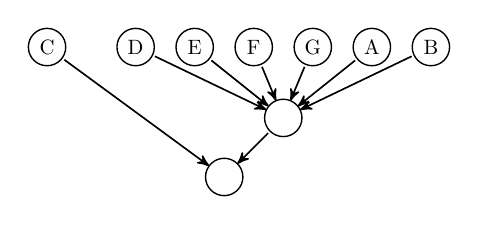
\begin{tikzpicture}[scale=0.75,transform shape]
		\tikzstyle{LabelStyle}=[fill=white,sloped]
		%  \tikzstyle{EdgeStyle}=[bend left]
		\Vertex[x=-2,y=0]{C}
		\Vertex[x=-0.5,y=0]{D}
		\Vertex[x=0.5,y=0]{E}
		\Vertex[x=1.5,y=0]{F}
		\Vertex[x=2.5,y=0]{G}
		\Vertex[x=3.5,y=0]{A}
		\Vertex[x=4.5,y=0]{B}
		{
			\SetVertexNoLabel
			\Vertex[x=2,y=-1.2]{H}
			%\SetUpVertex[FillColor=gray!70]
			\Vertex[x=1,y=-2.2]{J}
		}
		\tikzstyle{EdgeStyle}=[post]
		\Edge[](D)(H)
		\Edge[](E)(H)
		\Edge[](F)(H)
		\Edge[](G)(H)
		\Edge[](A)(H)
		\Edge[](B)(H)
		\Edge[](H)(J)
		\Edge[](C)(J)
		%  \Edge[label=$$](K)(F)
	\end{tikzpicture}
	\caption{\label{fig:key}Musical Key}
\end{figure}

One usually says that compositions are in a particular key, for example, ``Waltz in C-sharp minor.'' We can consider it equivalent to say that musical compositions are in a particular identity context. As such, some natural generalizations that could be explored include keys other than major and minor (such as the chromatic keys already discussed), and musical contexts composed of multiple keys (such contexts are no doubt already in use). Such a characterization could enable the study of the existing rules of music in a generalized form that could be applied in other non-standard tunings such as 19TET or forms of just temperament (musical set theory seems to be already applied in this manner). Additionally, by treating a chromatic key as a world and more specific keys (e.g. \emph{C major}) as minds within that world, it seems to be the case that musical transformations such as transpositions and modulations can be achieved by successive application of expression and perception functors.

Similarly, rhythm can also be interpreted in terms of identities. For example, the standard interpretation of the $\frac{6}{4}$ time signature ($6$-count) as distinct from the $\frac{3}{4}$ signature ($3$-count) -- that the emphasis on the first three beats is different from the second three beats -- appears to correspond to a characterization as a hive identity derived from $3$-count and $2$-count, and having aspects of both. Lewin in \cite{gmit} studies both musical notes and rhythms in terms of an abstract group-based structure he calls a Generalized Interval System (GIS). This unity in the mathematical structures of melody and rhythm seems to further ground the case for the applicability of identities to rhythm as well.

Finally, musical compositions are constructs that usually possess some high-level defining structure: a song may be composed of recurring sections such as a verse and chorus. Within each of these sections are distinct phrases consisting of particular melodies along with the accompanying harmonies, each of which of course consists of notes (generally) in the given key. At the highest level this entire structure may comprise a single movement, of which the composition may have several (in classical music, for example). And at the lowest levels, melodies and rhythms may possess further ornamentation -- melodies within melodies, and rhythms within rhythms, as especially evident in the Carnatic and Hindustani classical traditions. In all cases, the nested patterns must ``fit'' into the higher patterns if the identity of the higher pattern is to be expressed. As such, at a high enough level, there must exist a single meter into which all the patterns fit, which unifies and reinforces its identity as a single composition, as opposed to being just an overlapping multitude of musical patterns. This is indeed usually the case. This ``fractal'' structure in music betrays its ties to identities, and suggests that each level described may be studied independently in terms of identities. In music theory, Schenkerian analysis\cite{schenker} studies this type of nested structure.

There have been several other mathematical examinations of music and musical elements, for e.g. \cite{musicmath} and \cite{musselfsim}. As music is a cognitive phenomenon, we believe it must be the case that identity representation provides the basis for this mathematical structure.

\subsubsection{The Sense of Smell} \label{sec:sensme}

Similar identity abstractions can be found in our experience of the sense of smell. Different foods, for example, have different smells that we can pick out. Garlic smells a certain way, and onion another. Fish has a particular smell, as does sesame oil, truffle oil, mustard, chicken, steak, rice. But when we smell our favorite food -- eggplant curry, say -- as we are about to eat it, we don't smell the onion and the garlic and the eggplant. We smell \textit{eggplant curry}. Certainly, we could pick out the garlic within that smell just as we can pick out individual musical notes in a chord if we try. But our olfactory experience of the eggplant curry is a distinct one in its own right. Additionally, things could smell ``like Chinese food'' which corresponds to an anonymous identity (perhaps this anonymous identity includes soy sauce as a constituent) rather than a particular Chinese dish. As a more general example of this principle, we point to the familiar experience of being unable to discern the smell of a living space (or one's own smell, even) after being in it for a long time, while others are perhaps aware of its distinctive smell at first encounter. This can be seen as being due to that smell infusing and forming part of every other smell in the space, and thus, as a common ancestor, being constituent in the anonymous identity of smells in relation to inhabitants. As another example, the formulation of perfumes apparently follows identity construction -- different molecules possessing desirable smells are combined to create a unique olfactory experience (i.e. a hive identity) deriving from the properties of each of those molecules\cite{smellmolecules}.

\subsubsection{The Sense of Taste} \label{sec:sentas}

Food preparation is the practice of taking a number of ingredients and preparing them, putting them together in certain ways to create something that is more than the sum of its parts. If eggplant curry simply tasted like eggplant and like garlic and like onions, then one may as well eat each of those things separately, in any order. But our experience of the eggplant curry is quite different, and rather more enjoyable, than of any of its ingredients. Each dish is experienced as a hive identity comprised by its ingredients. Just as in music, where two notes may sound dissonant when played together, but consonant when played as part of a more complex chord, so it is with food where ingredients that may taste bad together by themselves (e.g. wasabi and soy sauce) can taste good when part of a more complex preparation (sushi).

\subsubsection{The Sense of Sight} \label{sec:sensig}

Our perception of color exhibits identity structure. Red and blue combined is purple -- a new color with a unique experience, distinct from either of its constituents. In other words, colors when combined yield other colors -- an obvious but noteworthy state of affairs. Our visual perception of objects can also be seen as exhibiting identity structure. Visual perception is entirely in terms of colors, contrasts, intensities in a two-dimensional matrix. But we don't see just colors and contrasts, we see \textit{things} -- books, laptops, people, cats. Each of these objects in our visual experience corresponds to a hive identity possessing various characteristic features which are themselves composed of characteristic features, and so on. A person could be characterized as having black hair (a purely visual characterization, irrelevant outside of visual perception), wearing a t-shirt. Black hair itself would have attendant features such as textures and reflectivity and spatial relationship with other identities such as face and body. In the field of computer vision, probabilistic models are developed to identify objects in scenes. Such models could benefit from a basis in identity architecture, and also be generalized to represent all of perception and reasoning, since after all, all forms of perceptual representation and reasoning are (we believe) in the same terms -- that of identities. This envisioning is consistent with proposals by Mountcastle\cite{mountcastle} and by Hawkins\cite{hawkins}.

\subsubsection{The Sense of Touch} \label{sec:sentou}

If we close our eyes and run our hands over an unknown object in our vicinity, we naturally develop a characterization such as ``a small box with a smooth top and a coarse bottom, with a metallic latch.'' When we compare this to the actual sensory input which could be expressed as something like ``edge, corner, edge, corner, smooth, edge, corner, rough, edge, cold,'' it's easy to see that the sense of touch also is in the hierarchical terms of identity. In the sense of kinesthetics, identities manifest in our execution of complex physical maneuvers such as playing sports, engaging in martial arts, dancing, acrobatics. These could all be seen as corresponding to identity trees composed of all the attendant minute motions. When we pick up a pen that has fallen to the ground, we don't imagine moving our hands and fingers together with our arms and waists and knees and straightening out by shifting our weight a certain way and then placing the pen back on the table in another subtle and clever hand-and-arm gesture. We simply think of picking up the pen and putting it back on the table -- a hive identity we constitute by all those minutiae in an identity tree. The actual performance of the act can be seen as an i-morphism from this identity structure in the mind to the set of endomorphisms of the relevant identity structures in the world (including even our own physical form), i.e. an identity action as described in \autoref{sec:matmod}.

\subsection{Privacy} \label{sec:privacy}

Identities motivate a natural model for privacy; indeed, privacy itself may be seen as derivative of intrinsic notions of identity. Actions of an identity (in both the literal and algebraic sense) on other constituents in a context give rise to genesis of new identities, and we consider this to fully characterize how information is manifested in a context.

In natural phenomena, identity contexts emerge implicitly (i.e. via genesis; also see \autoref{sec:natphe}), while in human societies, contexts emerge implicitly but can also be conceived of in a persistent way, and actions can be taken in accordance with these perceived identity contexts (which we referred to as ``absolute'' contexts earlier). For example, if a citizen of a small town were to stand in the town square and make a proclamation, citizens of the town who are witness to it feel free to discuss it with other townsfolk who were not present there. They understand that proclamation to have occurred in the mind of the town as a whole. In comparison, if one individual were to make a private disclosure to another (``I'm Batman.''), the latter would generally feel impelled to share that disclosure with no one else; that is, both individuals represent this disclosure to have occurred in the mind constituted by just those two individuals. It's a ``secret.'' We observe in passing that secrets as identity contexts can have (as is familiar) any number of participants (constituents) (``I'm only telling you guys -- don't tell anyone else''), but due to anonymous effects (\autoref{sec:anoide}), a secret is only enforceable in the physical world if it is shared between a maximum of two individuals.

\begin{figure}[htp]
	\centering
	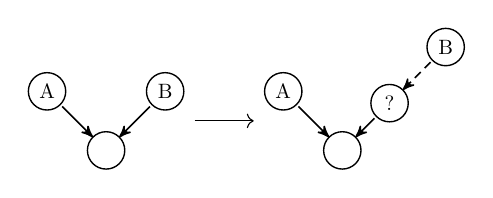
\begin{tikzpicture}[scale=0.75,transform shape]
		\tikzstyle{LabelStyle}=[fill=white,sloped]
		%  \tikzstyle{EdgeStyle}=[bend left]
		% original
		\Vertex[x=-3,y=0,LabelOut=false]{A}
		\Vertex[x=-1,y=0]{B}
		{
			\SetVertexNoLabel
			\Vertex[x=-2,y=-1]{C}
		}
		\tikzstyle{EdgeStyle}=[post]
		\Edge[](A)(C)
		\tikzstyle{EdgeStyle}=[post]
		\Edge[](B)(C)

		\draw [->] (-0.5,-0.5) -- (0.5,-0.5);

		% dissociated proxy
		\Vertex[x=1,y=0,LabelOut=false,L=A]{A'}
		\Vertex[x=3.75,y=0.75,L=B]{B'}
		\Vertex[x=2.80,y=-0.20,L=?]{D}
		{
			\SetVertexNoLabel
			\Vertex[x=2,y=-1]{C'}
		}
		\tikzstyle{EdgeStyle}=[post]
		\Edge[](A')(C')
		\Edge[](D)(C')
		\tikzstyle{EdgeStyle}=[post,densely dashed]
		\Edge[](B')(D)
		%  \Edge[label=$$](K)(F)
	\end{tikzpicture}
	\caption{\label{fig:privacy}Association/Dissociation}
\end{figure}

We propose the following properties for the evolution of persistent identity contexts:

\begin{enumerate}

\item Within a context, an identity may declare or revoke an association to a child identity at any time. This results in a new child context with the modified tree. (\emph{association})

\item Any thought can act through the self\footnote{The precise mechanism by which a thought can act through the self of a hive identity, as noted elsewhere, is to be specified in future work.}. (\emph{presentation})
	\begin{enumerate}
		\item An identity can act through any of its descendants (but descendants cannot act through ancestors).
		\item An identity can act through a ``dissociated identity.'' Acting through a dissociated identity is equivalent to acting anonymously in the world, but with the ability to ``reclaim'' the action being preserved.
	\end{enumerate}

\item All things in a world should be accessible as thoughts in every mind within that world; i.e. all information in a world is ``public'' with respect to every constituent. (\emph{perception})

\item World-representations of any thoughts that are not descendant from the self (and which are not mind-representations of things) should be trivial. In other words, identity trees within a mind should not in general be accessible from the world. (\emph{privacy})

\item It should be impossible (``hard'') to identify as descendant from a non-ancestor identity. (\emph{authentication})

\item It should be impossible (``hard'') to assert the association of an identity with one of its ancestors or descendants if that association has not been declared. (\emph{confidentiality})

\end{enumerate}

The first four properties are the core aspects, capturing and generalizing our everyday intuitions about privacy in human interactions. The first two enable Bruce Wayne and Batman to be two separate people to the world, and the same person to a few trusted aides. These can also be thought of as enabling an identity to act via a distinct ``identity proxy'' for each action it takes in the world, and further enabling the ability to associate or dissociate these proxies (and the associated actions) at any time. This type of pruning of one's identity tree could be seen as an explicit construction of one's so-called ``narrative identity''\cite{narrativeidentity} and is stronger than what we are practically able to achieve in human interactions in the physical world. The third and fourth properties ensure our intuitions about what we consider to be shared information, and what information should not be accessible outside a privileged context (note that these are relatively defined and support these notions of privacy in a self-similar manner at every level). These and the last two properties ensure integrity of the identity architecture and may be accomplished cryptographically. For this purpose, schemes based on Identity-Based Encryption (IBE) as proposed by Shamir\cite{shamir} and developed by Boneh and Franklin\cite{boneh} and by Cocks\cite{cocks} may be applicable.

Within a particular world $\mathcal{W}$, as already discussed, the anonymous identity $\varnothing_\mathcal{W}$ of that world is an ancestor of all identities in that world. This implies that the anonymous mind context ${\mathcal{M}}_{\varnothing_{\mathcal{W}}}$ contains a faithful representation of all non-anonymous minds within $\mathcal{W}$ (as described in \autoref{sec:awamem}). We call an identity \emph{omniscient in $\mathcal{W}$} if it has access to this anonymous mind ${\mathcal{M}}_{\varnothing_{\mathcal{W}}}$. By the requirement $2(a)$ above, only a supremum of all ancestors of $\mathcal{W}$ in $\mathcal{W}_1$, and its ancestors, would have such access; and in general no identity in $\mathcal{W}$ would have access to ${\mathcal{M}}_{\varnothing_{\mathcal{W}}}$. This supremum in $\mathcal{W}_1$ may be the $\mathcal{W}_1$-anonymous identity $\varnothing_{\mathcal{W}_1}$ itself, in which case we would have to continue, possibly indefinitely, to outer worlds until a non-anonymous supremum is reached, in order to find a non-anonymous identity (i.e. one that is in a position to ``act,'' since no nontrivial action can be defined directly on an anonymous identity, just as no nontrivial function can be defined on the empty set) that is omniscient in $\mathcal{W}$. By considering the world of human affairs, this reasoning ensures that, in general, no centralized authority \textit{in the world} having access to all information would exist. In particular, as will be elaborated in \autoref{sec:humins}, a nation is a hive identity in the world and is therefore a \textit{descendant} of its citizens. As a result, a nation, in particular, is not omniscient in $\mathcal{W}$ and therefore should not have access to the affairs of all of its citizens, unless for activities in which those citizens happen to be acting on behalf of the State, such as on diplomatic missions. Additionally, the model implies that elected representatives are representations of the hive identity constituted by a subset of citizens (and approximated by a human individual in political systems such as representative democracy). Therefore the activities of the representative -- acting in his capacity as representative -- should be treated as the actions of this hive identity, and in particular should be fully known to all constituents.

We also observe that while hive identities composed of humans is obviously a useful abstraction that has been applied throughout human history, it has seemingly always been dissociable in practice into its constituents (e.g. a corporation, tribe or nation) or embodied by a single individual (e.g. an elected representative), which can make the hive identity only implicit in some sense. But with the aid of cryptography we could \textit{guarantee} that such an identity is not dissociable into constituents, and so there would be no inherent way to distinguish an identity composed of $100$ humans (or a billion humans) from a single human, making such a hive identity as ``real'' a person as a human under a reasonable abstraction of personhood\footnote{Note that corporations, nations, and other such extant ``human institutions'' (see \autoref{sec:humins} for further development) are only crude approximations of the identity model, and these considerations of personhood do not apply to them. On the other hand, it is likely that the identity model is exactly implemented in the brain, basing the privileged status of personhood accorded to humans.}.

\section{Commentary and Conjecture} \label{sec:comcon}

\subsection{On the Experience of Living} \label{sec:expliv}

In the universe, there are phenomena that are meaningful at vastly different scales of space and time. The scale of billions of years in time is that at which the evolution of the universe and of life is meaningful. The scale of hundreds of thousands of light-years is that at which the structure of galaxies is a worthwhile study. These scales are almost unimaginable in the context of our everyday experience; still, our human scale is equally inconceivable and strange to a microorganism. The world experienced by a bacterium is one without books, desks, trees or buildings (as useful, emergent models). And yet these are such familiar features of our experience as humans. The scales that we consider to be ``reasonable,'' then, are not privileged in any intrinsic way. Our perception of them as ``normal'' would be entirely arbitrary if it were not for the fact that it is at these human scales that our actions yield tangible outcomes. It is at these scales that our influence is meaningful, and where our pursuits are tractable. The scale at which we operate, it seems, is dictated precisely by the scale of our influence.

This awareness of the arbitrariness of scale is intrinsic in our functioning, and intuitively apparent to every person on Earth. The following statements may serve to illustrate that we have no trouble adjusting the scale of our conceptions in everyday life:

\begin{enumerate}
	\item ``Look at this scratch on the cup here, next to the handle.''
	\item ``I heard a fire engine nearby.''
	\item ``San Jose is not far from San Francisco.''
	\item ``Alpha Centauri is a nearby star.''
	\item ``The Andromeda Galaxy is quite close to us.''
\end{enumerate}

\textit{Close to us.} We are speaking of something a million light-years away, but it sounds perfectly harmless to say that it is nearby. What is the implied identity here that we are embodying? It is not of ourselves as humans, but as a galaxy -- the Milky Way. It can be seen that the scale of our everyday existence is an arbitrary one that just happens to be so convenient as to be the one we embody almost all the time. We are perfectly capable of embodying identity at any scale -- and, indeed, it is quite likely that as our experience of living evolves in the years ahead, these scales will vary so widely as to render arbitrary even in practice any particular choice (such as the human scale) in this regard.

On another note, we observe that in life certain choices, such as crossing the road at this intersection or the next one, for the most part do not affect one's global trajectory through life at all (despite the possibility of serendipitous, life-changing encounters by crossing at this intersection, the likelihood of such chance encounters can be considered small enough to be negligible), while other choices, such as deciding to attend either of two universities, may dramatically alter the course of one's life. Both of these examples are binary decisions, and yet qualitatively they are clearly very different. These can be differentiated by the nature of their genesis: the former choice rapidly reaches the trivial action in a short amount of time, i.e. both alternatives terminate within the mind representing simply that we crossed the road at all, thereby not changing one's trajectory appreciably; while the different minds (i.e. whose actions on the world are different) resulting from the latter choice converge in a common mind only on much larger scales -- in a few decades or centuries it may not matter which university one decided to go to. Along the same lines, the actions entailed in the genesis of a major meteor impact reverberate for millions of years before terminating. Of course, it need not be the case that genesis must always terminate\footnote{Further algebraic development of action and reaction will be needed to shed light on the conditions under which genesis will terminate.}. % elaborate commutative / non-commutative

\subsection{On Natural Phenomena} \label{sec:natphe}

We directly perceive the world through the senses available to us. Over time, we've developed an understanding of the phenomena in nature that trigger these sensations (chemical interactions for taste and smell, pressure waves for hearing, and photons for sight), and now with this understanding we are comfortable treating the sensing of these phenomena by scientific instruments as extensions of our own senses. When the Hubble Space Telescope takes a picture of a distant galaxy, we are able to look at that picture and immediately interpret it as what that object would ``look'' like if one were near enough to be able to see it at the scale of the photograph. Similarly, there are things smaller than the eye can see, but which can be seen by specialized instruments and which, when presented to us, are interpreted as if we had seen these things ourselves with our own eyes. We've also discovered other phenomena that we cannot sense directly, but whose existence we infer by their interactions with those things that we do sense. Once again, instruments we construct to detect these phenomena serve as extensions of our senses -- probes into a universe that evidently exists out there.

But once we conceive of things they become thoughts, and whatever may exist out there, our experience of it resides entirely within. The substance of our experience is identities, and so, to the extent that the mind is an accurate representation of the world -- that is to say, to the extent that the perception functor between the physical world and our (human) minds is an \textit{equivalence} -- natural phenomena, too, can be characterized by identities.

We can begin to speculate on such a characterization. As a start, the mechanism of genesis can be construed as an ``algebraic'' or ``computational'' basis for natural phenomena (a computational approach to natural phenomena has been considered previously, for example as described in \cite{greatideas} and \cite{wolfram}). Objects in the universe, as already indicated, can be seen as identities, and phenomena as their actions. As an example of this, in solids, changes in temperature cause rapid and complex changes in atomic motion, but the emergent experience of this motion is barely perceptible and for the most part the solid is still ``the same'' in its large-scale interactions. The complexity of interactions resulting from atomic motion can be said to be encapsulated in a ``terminal mind'' that is small relative to the scale of the macroscopic identity, and whose contribution to the emergent macroscale action of the solid varies tractably. This can be seen as rather a general principle applying to all emergent phenomena in relation to component interactions, in particular providing a formal framework within which to justify division of scientific endeavor into different fields of study at different scales, as we do in our extant divisions of physics, chemistry, biology, sociology, and so on.

The `actual' existence of space and time has been a subject of investigation in philosophy since the beginning. On the one hand it is tempting to assume their existence, but on the other, such an assumption constitutes a strong claim about reality, one that philosophers have felt the need to either justify with equally strong arguments, or abandon. According to \cite{waite}, Shankara held that space and time are creations of Maya (i.e. the epistemic representation) and are thus ``unreal.'' Kant expressed a similar view, that space and time are \emph{Anschauung}, literally ways of ``looking at'' reality\cite{russell}, and are a priori (i.e. in the mind) rather than empirical. Einstein is partial to this view, proposing that conceiving reality as a unified field may make the need for a separate conception of space and time superfluous. He summarizes, ``space-time is not necessarily something to which one can ascribe a separate existence, independently of the actual objects of physical reality.''\cite{einstein} In favoring the buddhist \emph{citta-matra} position that consciousness is the `element' of nature/reality (see \autoref{sec:phicon}), and the \emph{sunyata} position that existence is definitionally relative, we are inclined towards such a denial of space and time. It seems economical (and thus appealing) to assume that identities, actions, and emergent contexts can suffice as a theoretical representation of the structure of reality, without necessitating an additional conception of time and space. Each point in ``space'' can be taken to specify a unique context at a particular point in ``time,'' with all identities in that context being characterized by instantaneous actions that vary continuously with ``motion'' in ``space'' (i.e. under certain algebraic actions, e.g. those corresponding to `motion' by the observer). The algebraic flow of causation may sufficiently explain phenomena without recourse to an additional independently-existing notion of ``time,'' which may be well-specified only as a relational quantity between two frames. If at any rate space and time must be assumed to actually exist, then at the very least, these assumptions should be framed as axioms with some assignable epistemic priority (\autoref{sec:epipri}).

Another way to think about this is that in any context, there are identities that are well-defined in relation to it, i.e. which ``exist.'' For example, buildings, people, astronomical bodies may be taken to exist in this sense. The interactions of these identities occur at many levels, all of which have manifestations that we categorize as ``spatiotemporal.'' This suggests that most identities in conscious experience, in particular those that are dialectical, have a common identity ancestor\footnote{This ancestor, being of ``universal'' type (\autoref{sec:onuni}), may exist in some mind in relation to the dialectical contexts under consideration (e.g. a ``human'' mind), rather than exist in (i.e. be defined in relation to) these contexts themselves, if the intimations in \autoref{sec:onuni} are sustained.} whose interaction we would describe as spatiotemporal in this conventional sense (and which indeed would represent our \textit{definition} of spatiotemporal), and as such, we can think of spatiotemporal interaction as the interaction of the identities under consideration when transformed under a forgetful functor into the mind of this anonymous ancestor. There may be identities that do not interact spatiotemporally in this sense, i.e. which do not share the spatiotemporal ancestor with other conventional dialectical objects of reality.

In light of this conception, entangled elementary particles could conceivably be modeled as such non-spatiotemporal identities, possibly as a hive identity where the ``separate'' particles may be seen to act as a single identity, while the states of the individual particles are simply undefined (in fact possibly undecidable, from \autoref{cor:decidability}) in the physical world. As there is no notion of ``space'' involved, the possibility of non-local correlations presents no difficulties.

In relativity theory a foundational idea is the principle of relativity -- that the laws of physics in a suitably defined reference frame are indistinguishable (e.g. by any experiment) from those in any other frame. This is a principle adopted largely on aesthetic grounds, but also due to the strength of its implied results and the simplicity of derivations enabled by it. Thus, the principle is adopted at least partially on utilitarian grounds. Alternatively, within the framework of epistemic priority, it may be seen that relativism (idampratyayata) arises at a very high priority. As a result, the framework provides an epistemic basis for favoring this principle. Not only that, but due to the priority of the principle and (perhaps consequently) due to its ``radically general'' nature, it may be seen that relativity of the \emph{physical} kind is only a particular manifestation of this much more general definitional relativism. A manifestation of this in the specification of identity architecture is that all identities are qualitatively equivalent and defined in relation to a context. It seems likely that the physical principle of relativity may be \emph{derived} from these foundational axioms that apply universally, via an appropriate transformation of identity actions.

It is conceivable that along this axis of development, physical reference frames may be modeled as contexts obtained via forgetful functor applied to the objects of reality to retain only their spatiotemporal interactions. The Lorentz transformation, being a linear transformation in spacetime, could be treated as deriving from a mind/world adjunction across identity contexts\footnote{A mind/world adjunction is concerned with \emph{actions} rather than spacetime coordinates and extension. Thus the transformation would have to be shown to derive from the mapping under a functor of the action of a generic spatio-temporal identity (Poincar\'{e} group?) between contexts.}.

The mechanism of genesis is inherently dynamical, and could possibly be applied to the characterization of dynamical systems and chaos. Any results derived here would be functorially transformable into results about social systems, biological systems, and even cognitive systems.

Energy is an abstract, even philosophical concept in physics. It is considered to be present everywhere in all things while itself remaining formless, ineffable. These properties appear to describe an anonymous identity, and it is thus tempting to consider the latter as the underlying model. We then infer things in the universe to be the (non-anonymous) manifestations of the energy identity -- its descendants in a bodhitree. And by the mass-energy equivalence, everything that exists in the universe can indeed be said to be a manifestation of energy, just as all identities in a context are manifestations of, or defined in relation to, an anonymous identity (and more specifically, a brahman). A precise characterization of energy in the physical world, like money in human societies, in terms of anonymous identity, could be a worthwhile and integrating effort. It seems likely that full characterization in this regard would have to quantify the relationship to entropy as well, which it's possible will be facilitated by an information-theoretic development.

We close with the observation that identity architecture as a model is scale-invariant. As such, the same principles that apply at one scale are the ones that apply at any other scale (though possibly encoding radically different behavior). Identities could therefore conceivably underpin, and thereby constrain, theoretical models of phenomena in widely varying regimes such as the subatomic, molecular, and biological regimes, all the way up to human and cosmological scales of experience -- and presumably, beyond. Towards this end, we can envision our experience of nature as a (possibly non-denumerable, nonlinearly ordered) hierarchy of worlds that we inhabit to varying degrees. One such envisioning may be as follows: Cosmological $\rightarrow$ Filamental\footnote{Referring to filaments and galaxy clusters, thus far the largest known structures in the universe.} $\rightarrow$ Clusteral $\rightarrow$ Galactic $\rightarrow$ Stellar $\rightarrow$ Astronomical $\rightarrow$ Geological $\rightarrow$ Ecological $\rightarrow$ Sociological\footnote{including hive structures in the animal and plant kingdoms} $\rightarrow$ Biological\footnote{A forgetful functor from \textbf{Soc} to \textbf{Bio} could be said to result in the ``State of Nature'' discussed by political philosophers since Hobbes.} $\rightarrow$ Chemical $\rightarrow$ Physical $\rightarrow$ Noumenal\footnote{Kant's\cite{kant} ``noumenal world'' of ``things in themselves'' -- things without ascribed structure in relation to us; a useful limiting idealization.}; where each $\rightarrow$ is a forgetful functor that ``forgets hives'' in the preceding world. We could follow the convention from category theory in employing abbreviated boldface for each of these worlds, e.g. \textbf{Cos} or \textbf{Phys}. As conscious agents, we are able to embody nontrivial minds in a subset of these worlds, such as in the sociological and the ecological worlds. Interestingly, if two contexts at different scales entailing an ancestor-descendant relationship (e.g. protein interactions in a particular cell, and interactions between cosmological filaments) were found to be isomorphic, then the possibility of infinite semantic extent of the cosmos appears to follow.

\subsection{On Human Institutions} \label{sec:humins}

As we saw in \autoref{sec:natphe}, reality in relation to us is structured by our representation of it, and thus natural phenomena to the extent that they are perceived must conform to description in terms of this representational framework, i.e. (we propose) in terms of identities. But our experience of reality is not altogether passive -- some processes in nature were put in place by us. These processes also trivially conform to description in terms of identities, but in addition they can be said to possess structure representing a latent and emergent (yet still nascent) conscious understanding of identity architecture. Let us now embark on a study of these in particular as the class of identities that correspond to human institutions.

\subsubsection{Social and Political Systems}

The institution of family is perhaps chronologically the first that we become aware of. A family can be seen as a hive identity comprised by its members -- a married couple and their children, say -- which sustains within it all possible combinations of hive identities as provided in the definition of an identity context. In particular, within the mind of a family of four, say, can exist a hive comprised by the parents alone, by the parents and the children, the children alone, each child with each parent, each child with both parents, and so on. This corresponds to the familiar fact that every combination of members of a family entails a unique relationship not encompassed by the hive comprised by all members alone. For example, parents may have all sorts of conversations and considerations that their children are never privy to, and vice versa. Additionally, it can be seen that the institution of family entails the dominant duality ``parents and children,'' which mitigates anonymous effects that may otherwise emerge in a hive of order $\geq 3$. The institution of marriage itself will be touched upon further in the section on \hyperref[sec:phirelhistra]{\textit{religious traditions}}.

In the wider world, we are part of hive identities that include close friendships, social groups, professional networks. In all cases, the same ``power identity'' structures hold entailing all possible combinations of hive identities. These correspond to the unique relationships and privacy domains (i.e. contexts) defined by each relationship that we cultivate in the world.

In the past, larger functional hive identities constituted by humans included tribes, and as the scale of our influence grew we created larger structures still. Tribes constituted settlements, settlements grew into towns, towns to cities, and cities into nations. As such, nations as they exist today can be seen to be hive identities constituted by states, which are hive identities constituted by counties and cities, which are hive identities constituted by people (which, for many purposes, are hive identities constituted variously by ideas (related: Dawkins' ``memes''\cite{dawkins}), biological or chemical constituents, or other constituents depending on context). More precisely, as people often directly constitute both states as well as nations, nations can be said to be hives constituted by people and states, with the states being constituted by nonintersecting subsets of the people. Yet another characterization is that people constitute states which together constitute a federation. Independently, people all together constitute what could be called a ``commonwealth.'' The nation, then, is the hive formed by the federation together with the commonwealth. These different possible models are depicted in Fig.~\ref{fig:nation}.

As members of these geopolitical hives, we call ourselves ``citizens.'' That is, a citizen is a representation of a person in the mind of a particular geopolitical hive. Today as our scale of influence grows ever larger, we find that nation identities too are coming together to form larger hives still, such as the European Union and the United Nations\footnote{The question of what the functioning of these super-national hives ought to be has not yet, as far as we are aware, received a satisfactory specification, with the result that their implementation has proven to be challenging and uncertain. It seems likely that a formal understanding (and further development) of identity architecture may facilitate clarity on the matter.}.

\begin{figure}[htp]
\centering
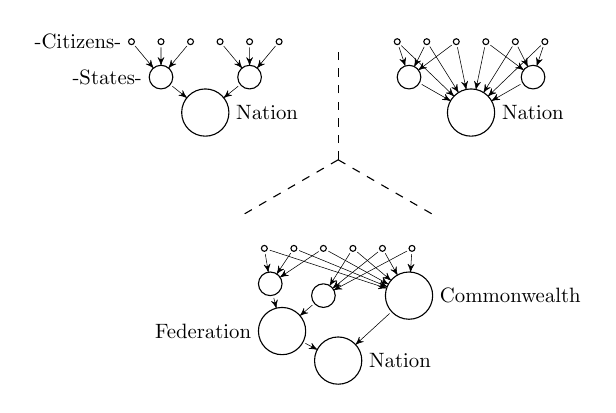
\begin{tikzpicture}[scale=0.75,transform shape]
  \tikzstyle{LabelStyle}=[fill=white,sloped]
  % bounds
  %\tikzstyle{EdgeStyle}=[dashed]
  \draw [dashed] (0,0) -- (0,1.9);
  \draw [dashed] (0,0) -- (1.6455,-0.95);
  \draw [dashed] (0,0) -- (-1.6455,-0.95);
  \tikzstyle{EdgeStyle}=[post,very thin]
  % model TL
  \tikzset{VertexStyle/.style = {draw=black,shape=circle,minimum size=0.1cm,inner sep=0pt}}
  \Vertex[x=-3.5,y=2.0,LabelOut=true,L=-Citizens-,Lpos=180]{c11_1}
  \SetVertexNoLabel
  \Vertex[x=-3.0,y=2.0]{c12_1}
  \Vertex[x=-2.5,y=2.0]{c13_1}
  \Vertex[x=-2.0,y=2.0]{c21_1}
  \Vertex[x=-1.5,y=2.0]{c22_1}
  \Vertex[x=-1.0,y=2.0]{c23_1}
  \tikzset{VertexStyle/.style = {draw=black,shape=circle,minimum size=0.4cm,inner sep=0pt}}
  \SetVertexLabel
  \Vertex[x=-3.0,y=1.4,LabelOut=true,L=-States-,Lpos=180]{s1_1}
  \SetVertexNoLabel
  \Vertex[x=-1.5,y=1.4]{s2_1}
  \tikzset{VertexStyle/.style = {draw=black,shape=circle,minimum size=0.8cm,inner sep=0pt}}
  \SetVertexLabel
  \Vertex[x=-2.25,y=0.8,LabelOut=true,L=Nation]{n_1}
  \Edge[](c11_1)(s1_1)
  \Edge[](c12_1)(s1_1)
  \Edge[](c13_1)(s1_1)
  \Edge[](c21_1)(s2_1)
  \Edge[](c22_1)(s2_1)
  \Edge[](c23_1)(s2_1)
  \Edge[](s1_1)(n_1)
  \Edge[](s2_1)(n_1)
  % model TR
  \SetVertexNoLabel
  \tikzset{VertexStyle/.style = {draw=black,shape=circle,minimum size=0.1cm,inner sep=0pt}}
  \Vertex[x=1.0,y=2.0]{c11_2}
  \Vertex[x=1.5,y=2.0]{c12_2}
  \Vertex[x=2.0,y=2.0]{c13_2}
  \Vertex[x=2.5,y=2.0]{c21_2}
  \Vertex[x=3.0,y=2.0]{c22_2}
  \Vertex[x=3.5,y=2.0]{c23_2}
  \tikzset{VertexStyle/.style = {draw=black,shape=circle,minimum size=0.4cm,inner sep=0pt}}
  \Vertex[x=1.2,y=1.4]{s1_2}
  \Vertex[x=3.3,y=1.4]{s2_2}
  \tikzset{VertexStyle/.style = {draw=black,shape=circle,minimum size=0.8cm,inner sep=0pt}}
  \SetVertexLabel
  \Vertex[x=2.25,y=0.8,LabelOut=true,L=Nation]{n_2}
  \Edge[](c11_2)(s1_2)
  \Edge[](c12_2)(s1_2)
  \Edge[](c13_2)(s1_2)
  \Edge[](c21_2)(s2_2)
  \Edge[](c22_2)(s2_2)
  \Edge[](c23_2)(s2_2)
  \Edge[](s1_2)(n_2)
  \Edge[](s2_2)(n_2)
  \Edge[](c11_2)(n_2)
  \Edge[](c12_2)(n_2)
  \Edge[](c13_2)(n_2)
  \Edge[](c21_2)(n_2)
  \Edge[](c22_2)(n_2)
  \Edge[](c23_2)(n_2)
  % model BOT
  \SetVertexNoLabel
  \tikzset{VertexStyle/.style = {draw=black,shape=circle,minimum size=0.1cm,inner sep=0pt}}
  \Vertex[x=-1.25,y=-1.5]{c11_3}
  \Vertex[x=-0.75,y=-1.5]{c12_3}
  \Vertex[x=-0.25,y=-1.5]{c13_3}
  \Vertex[x=0.25,y=-1.5]{c21_3}
  \Vertex[x=0.75,y=-1.5]{c22_3}
  \Vertex[x=1.25,y=-1.5]{c23_3}
  \tikzset{VertexStyle/.style = {draw=black,shape=circle,minimum size=0.4cm,inner sep=0pt}}
  \Vertex[x=-1.15,y=-2.1]{s1_3}
  \Vertex[x=-0.25,y=-2.3]{s2_3}
  \tikzset{VertexStyle/.style = {draw=black,shape=circle,minimum size=0.8cm,inner sep=0pt}}
  \SetVertexLabel
  \Vertex[x=1.20,y=-2.3,LabelOut=true,L=Commonwealth]{cw_3}
  \Vertex[x=-0.95,y=-2.9,LabelOut=true,L=Federation,Lpos=180]{f_3}
  \Vertex[x=0,y=-3.4,LabelOut=true,L=Nation]{n_3}
  \Edge[](c11_3)(s1_3)
  \Edge[](c12_3)(s1_3)
  \Edge[](c13_3)(s1_3)
  \Edge[](c21_3)(s2_3)
  \Edge[](c22_3)(s2_3)
  \Edge[](c23_3)(s2_3)
  \Edge[](c11_3)(cw_3)
  \Edge[](c12_3)(cw_3)
  \Edge[](c13_3)(cw_3)
  \Edge[](c21_3)(cw_3)
  \Edge[](c22_3)(cw_3)
  \Edge[](c23_3)(cw_3)
  \Edge[](s1_3)(f_3)
  \Edge[](s2_3)(f_3)
  \Edge[](cw_3)(n_3)
  \Edge[](f_3)(n_3)
\end{tikzpicture}
\caption{\label{fig:nation}Nation Models}
\end{figure}

As discussed in \autoref{sec:theself}, actions of a hive identity in the world (like those of any identity) result from actions of the self in the mind. It appears to be the case that in current systems, this mechanism is approximated by forming, as a representation of the self of the nation, an identity we call the government. For actions of a government ``in the mind'' result in actions of the nation ``in the world'' (including activities pertaining to the territories and people considered to be under its jurisdiction), and a government does approximately correspond to a representation of the nation as it exists in the (geopolitical) world, in conformance with the definition of the self. This sort of envisioning is not a new idea, and was perhaps first clearly articulated by the philosopher Hobbes, who conceived a nation to be an artificial person he called ``Leviathan,''\cite{hobbes} and the sovereign (i.e. government; Hobbes favored monarchy) to be an ``artificial soul''\cite{russell}.

\subsubsection{Economic Systems}

In the Wealth of Nations\cite{adamsmith}, Adam Smith identifies three broad divisions in society: landlords, laborers, and merchants. Of these three, Smith observes that the interests of the former two are aligned with that of society (whether they know it or not), while those of the merchants are not necessarily so, and are indeed sometimes opposed to those of society\cite{rothschild}. A good portion of the Wealth of Nations is engaged in discussing the ramifications of this possible misalignment. Of course it goes without saying that the interests of merchants are not necessarily aligned with those of other merchants. The question of interests and incentives identified here is an important one that has engaged economists right up to the present day. Let us focus our energies toward a precise understanding of the issue. In order to achieve this, it will be necessary to frame the problem at a higher level of abstraction.

Let us assume that all members of society may indulge in any activities at any time. That is, they may be landlords in an abstract sense, of having possessions recognized as their property in society; or they may be laborers, in the sense that they engage in the direct execution of some tasks in the course of their daily lives; and they may be merchants, in that they may have projects and designs that they undertake over a relatively long timespan. Whether Smith's three-fold characterization is the best one is irrelevant for the purposes for which we intend to use it. The important notion is that for some subset of activities of this generic person, his interests are aligned with or independent of those of society, and for some subset of activities these interests are either partially or diametrically misaligned with those of society. Let us keep this in mind as we evaluate common economic systems in this connection.

Pure free market capitalism can be said to represent a formal model wherein each participant is assumed to act in self-interest, irrespective of considerations of alignment with other interests. That this is a gross simplification is evident, but it has the appeal of being a relatively well-specified quantitative model. It has the further appeal that under the idealized conditions assumed, the system incentivizes valuable contributions by virtue of recognizing these contributions to an extent that is approximately covariant with their true value as realized in the world. In practice the covariance of market value with true value is high only for some contributions; for many others it reflects a crude approximation, and in some cases it is not able to account for value at all and indirect measures must be resorted to (particularly for intangible contributions such as scientific works and the arts, where ``supply'' is poorly defined and thus market value is theoretically zero). Additionally, by aligning efficiency in production with market value, free market capitalism (as conceived here) achieves a convergence on global efficiency in production, but due to competition being adversarial in nature, also admits locally of waste and redundancy, with competing agencies replicating rather than sharing work. The free market is also able to cope with the fact that human society is nonlinear: activities and needs cannot be predicted effectively, and so determining and responding to these organically (through dynamic assignment of value) as the free market does is an elegant solution. On the other hand, under the same idealized assumptions, the system can be said to be always in a state of unstable equilibrium in the sense that a small advantage for a competitor can lead to the formation of a monopoly (which inhibits the ability of the system to recognize value), a feature that must often be curtailed by legal means. Finally, adversarial competition entails enormous legal and logistical costs in addition to the costs arising from redundancy already identified. Stallman\cite{stallmancombat} likens this aspect to ``combat.'' The analogy is apt as free market capitalism can indeed, it seems, be conceived as a specific instance of a generalized abstraction of war, making each participant -- to the extent of mutual divergence of alignment in interests -- an enemy of every other. Of course, it is largely true that the Darwinian forces entailed lead to technological advancement.

Communism and socialism can be formally characterized as doing away with all interests except that of the State. As a result, they trivially achieve alignment of interests since there is only one interest modeled. The mutual enmity inherent in capitalism is precluded since such enmity would only arise from misaligned interests. The price paid for this alignment, however, is the lack of any means to recognize -- and thereby incentivize -- valuable contributions. As a consequence, although the local redundancy and waste inherent in adversarial competition is eliminated by the sharing of resources and developments, globally there is no mechanism in the model to drive efficiency in production, nor innovation more broadly. Communism advocates equality in all things, with Marx and Engels\cite{marx} going so far as to essentially propose a uniform distribution of people across the land, as opposed to the ``unequal'' distribution represented by cities and towns\footnote{Of course, such a distribution of people has more to do with efficiency than inequality. This example is thus perhaps unwittingly representative of the priorities intrinsic in communism.}. What this amounts to is an assumption in the model that all participants are in fact indistinguishable (i.e. ``equal''), which is again a gross simplification. As a result of the actual state of affairs entailing diversity (i.e. ``inequality'') of all kinds, the model effectively sacrifices fairness for the sake of equality. The absence of a market also means that needs cannot be accounted for dynamically and only in a centralized manner that is inadequate for the complexity of society.

Just as social and political institutions may be seen as approximations of identity models, economic systems too can be seen as such approximations. We will shortly conceive an economic system formally based on identity architecture, and hope to motivate that such a system can overcome many of the shortcomings of other systems while simultaneously retaining their benefits.

\subsubsection{Property}

Property is defined in Webster's dictionary as ``The exclusive right of possessing, enjoying, and disposing of a thing.'' Considerations of the need for, and the nature, extent and purpose of such rights have given rise to different conceptions over the course of history. In Ancient Greece in the time of Pythagoras, ``property was held in common [\ldots] Even scientific and mathematical discoveries were deemed collective.''\cite{russell}. By the time of Aristotle, this was evidently no longer the state of affairs, with Aristotle advocating private property. In the 16th century, according to Russell, Hobbes maintained that ``The laws of property are to be entirely subject to the sovereign; for in a state of nature there is no property, and therefore property is created by government, which may control its creation as it pleases.'' Locke\cite{locke} later placed great importance on \textit{private} property, suggesting that ``The great and chief end of men uniting into commonwealths, and putting themselves under government, is the preservation of their property[.]'' Rousseau, and later, Marx\cite{marx} proposed to abolish private property in favor of, essentially, all property being owned by the State (and indivisible, in Marx).

The predominant modern conception is largely the one espoused by Locke, but the matter is clearly not conclusively settled, with Russell observing that Lockean notions of property derive from the idea that production entails ownership, which was a valid heuristic in pre-industrial times, but which has needed to be revised post-industrial revolution. We make the following reductive observations as guiding principles that may inform such a revision. The purpose of property is:

\begin{enumerate}
	\item To secure privacy (including the concomitant sovereignty).
	\item To secure the freedom to use certain things (in any manner one wishes to). % "in any manner one wishes to" follows from privacy/sovereignty
	\item To facilitate the fair appropriation of value (e.g. in particular in relation to the ``owner'').
\end{enumerate}

The first item is tantamount to ensuring in human society the formal relationship between mind and world, in particular as developed in \autoref{sec:privacy}. The third item will be addressed in the following section. That leaves the second, freedom of use. But before we can discuss this, we will need some theoretical development.

Reich\cite{reich} calls attention to ``government largess'' -- rights, benefits, subsidies, contracts and so on emerging from government -- suggesting that it ought to be treated legally as a form of property. Perhaps more important in his analysis is the inverse observation that ``[\ldots] all property might be described as government largess[.]'' Thus, ``government largess'' can be seen to be a general conception, of which private property is a particular manifestation. Now, identity architecture motivates a further generalization -- that government largess is a particular instance of a more general phenomenon, that of actions of the self of a hive identity in its mind\footnote{We suggested in \autoref{sec:idebra} that actions of the self in the mind actually manifest in the world, but this is with the caveat that the manifestation in the world is the image under the expression functor, and as such it's conceivable that the manifestation in the world is trivial. That is, even if the action of the self is non-trivial in the mind, the resultant action in the world may be to do nothing. Further mathematical development is needed to specify this precisely.}. We will term such actions \textit{resolutions}.

\begin{defn}[Resolution]
	A \emph{resolution} by an identity $Q$ is an action $\phi$ of the self $Q'$ of $Q$ in the mind of $Q$. This action corresponds to an action of $Q$ in the world (under the expression functor), which may be a faithful, partial or trivial representation of $\phi$.
\end{defn}

This generalization allows us to consider manifestations of this phenomenon in the mind of nations, but also in any other mind. As an illustration of this: A house may be acknowledged to be the property of a particular family in the world -- this acknowledgement is a resolution by the nation (i.e. an act of the government). Within that house -- more precisely, within the mind of the family inhabiting that house -- a particular book may be acknowledged to belong to one member, and a particular toy to another. This is a familiar aspect of social existence -- property is not only assigned by the government (even if the government is the only one to do so \textit{legally}); it is assigned, rather, via resolution by the concerned hive identity; in this latter case, recognition of the book and the toy as property are resolutions by the family. We may continue the reasoning outward, and envision that the land that is the property of a particular nation, say the United States, is so via resolution of a global geopolitical hive, which we may consider as reified in the United Nations.

Now with this notion under our belt, we return to the issue of freedom of use. First, we differentiate two forms of this: (1) Freedom to use a representation of a thing (i.e. the thought corresponding to that thing) in the mind, and (2) freedom to use the thing itself in the world. Recall that in the formal specification of identity architecture, all things in the world have a representation in all minds in that world (\autoref{lem:maya}). Thus, the freedom to use articles of the world in a particular mind (such as in the mind of one's family, at home) is inherent -- in other words, articles of the world cannot (and in practical implementation, must not) be barred from use in any mind in that world. However, the free use of an article of the world in a mind is in practice often difficult to achieve. Articles of the world may be limited in number (or unique), and difficult to reproduce. In these situations, one resolution is to consider that the thing in question represents a potential value to the world in its capacity as an article of the world. If it is the case that relinquishing this value in favor of facilitating exclusive use of the article within a particular mind is of greater value to the world, then the resolution made in the world to this effect can be seen as the basis for this form of private property. This is indeed the justification often cited for private property, that it is bestowed upon private parties with limited regulation because it is in the public interest to do so.

Now in regard to the freedom to use a thing itself in the world, it is necessary for the activity involving such use to be treated as a composite identity in the world with the article in question as a component. That is, the article in question forms part of the body of the activity-as-a-thing\footnote{Heidegger\cite{heidegger} suggested that objects in the world when employed by us as ``equipment'' fade from conscious experience as separate things. The conception that such objects together with the wielder form the body of a derivative identity offers a precise basis for this view.}. Among other things, this allows value from the activity to be channeled fairly, as will be discussed in the following section. The freedom to access and use an article of the world must be determined also by resolution of the world hive. In this case the resolution is not for exclusive use in the mind, but instead for exclusive use for a limited period or for a particular purpose in the world, i.e. which is publicly known, and furthermore, publicly conducted. For example, this may relate to use of shared public resources, or the permission to undertake a proposed project using public resources, such as construction or decoration of a public building or bridge for some purpose. Importantly, any member of the world is free to request or suggest such use of articles of the world (even anonymously), and all such activities involving things themselves in the world must be ``public'' in relation to the concerned hive (even if conducted anonymously). In geopolitical hives such as nations these sorts of activities are largely facilitated (if at all) by governments. Government today is a particular approximation of the self of a hive identity, and does not necessarily represent the correct, precise manner in which resolutions must be made. We will attempt a beginning specification of this process in the following section.

Finally we observe that in the case of intangible things such as scientific contributions, ideas, computer software, literary and musical works, that these are easily reproducible and highly portable, making both freedom of use in the mind and freedom of use in the world trivial, and largely conforming to the ideal formal conception in identity architecture -- an eminently auspicious state of affairs. However at the present time these are artificially restricted by ``intellectual property'' law including copyrights and patents, in an attempt to facilitate fair appropriation of value. This is certainly a worthy goal, and it is thus not surprising that such systems may appear warranted. But in consideration of the above identification of the purpose of property, we see that this approach essentially seeks to achieve fair appropriation of value (item (3)) by sacrificing freedom of use (item (2)) and sometimes privacy (item (1))\footnote{Unlike traditional, tangible, property under oft-employed simplifying assumptions, the considerations here are ``mixed,'' sometimes applying to the ``owner'' and sometimes to ``users.'' This should be understood to reflect the broader confusion regarding ideas of property, rather than a flaw in the present argument.}, and arguably often the ``fair'' part of appropriation of value.

In recognition of these problems, an alternative proposal for intangibles is Stallman's ``copyleft,''\cite{stallmancopyleft} which entails a general system applied primarily to works of software in which such works are made freely (as in ``freedom'') available for use and modification with the proviso that any such modifications must be made available under the same conditions. This system succeeds in achieving freedom of use in mind and world (item (2)), but the requirement in the system for derivative works in a mind to be made available in the world constitutes a compromise on privacy (item (1)) in favor of minimal guarantees of fairness (item (3)): that although fair appropriation of value cannot be ensured, unfair exploitation will be structurally precluded. The system does not provide additional guarantees of fair appropriation of value from derivative works.

While such compromises may appear to be warranted in order to achieve the stated goals, we do not believe that they are necessary, and propose that they can be avoided if instead fair appropriation of value is facilitated as described in the following section.

\subsubsection{A Universal System}

The above discussion is intended to illustrate that common institutions in human society can be seen as approximations of identity architecture-based ones. With formal specification of the relevant models, we can begin to construct these models explicitly, replacing extant manifestations with more precise implementations. We can envision what such implementations would look like, so as to point the direction for further work in this area.

%As we proceed in this conception, we identify three broad ideals to maximize: freedom, fairness, and truth; and where these may be in conflict, we propose to err on the side of fairness. This is justified in consideration that absolute freedom is not desirable since it imposes on the freedom of others, and absolute clarity of truth may be detrimental as motivated in the baker example of \autoref{sec:introduction}. Fairness is never in conflict with desirable outcomes. It is the eternal tiebreaker, the ultimate arbiter. As a clarification we point out that fairness is not the same as equality. Even ``equality of opportunity,'' while being fair, is not a comprehensive characterization of the much broader ideal of fairness.

\paragraph{Decision Making} Let us first consider the nature of decision-making in an institution. The precise manner in which thoughts in a mind -- in general -- interact to produce actions of the self, that is to say to produce resolutions, remains to be specified in future work, with direct applicability to the operation of institutions. For now we can outline a possible mechanism for institutions which is likely to be an approximation of the ``correct'' general (i.e. mathematical) one, and which should ultimately be disregarded in favor of a specialization of that more general mechanism:

\begin{enumerate}
	\item Activities involving things themselves in a world are subject to resolution by that world hive -- i.e. an action of its self.
	\item Any constituent is free to contribute to, make proposals for, and vote on any resolution.
	\item A ``vote'' will comprise applying an influence toward a candidate resolution (by forming a composite identity with it).
	\item Votes will be cast anonymously (i.e. via dissociated identities).
\end{enumerate}

When the aggregate influence applied on the most highly weighted course of action (which itself may be arrived at through composition of multiple provisional proposals) exceeds the opportunity cost for a subset of thoughts, those thoughts take on that course of action, and by doing so, would be acting not as themselves but as the self of the hive identity, effecting the will of the hive in the world. Note that as this scheme applies in every mind within the hive under consideration, it can be seen to provide essentially a recursive (``fractal''), weighted democracy. By the same token, if a particular thing concerned in the resolution cannot reasonably be treated as ``private property'' of the world hive in the sense described in the previous section, then any such resolution would still be provisional pending an identical process in the hives of outer worlds, until a ``containing'' resolution is passed in a world where the thing is indeed the ``private property'' of that hive. For example, archaeological sites may be treated as the property of humanity rather than of the particular nation within whose boundaries it may exist, and thus any resolutions in that nation regarding land and artifacts associated with that site would be subject to resolution by a hive representing humanity, for example something like the United Nations.

The voting is anonymous so that the best ideas and courses of action for the hive are selected without regard to their originator. At the same time, since those who are more invested and/or knowledgeable in certain issues will have greater influence in those issues (i.e. in the relevant identity contexts), the better ideas (as measured in the concerned hive mind) would indeed be more highly weighted in terms of influence, even though they are anonymous. This is a subtle point and worth elaborating further: how much say an identity has in a particular context is proportional to its wealth in the context (as defined in \autoref{sec:currency}). This is a desirable state of affairs \textit{under the assumption that the system is fair in the assignment of value}\footnote{This cannot be assumed to hold in extant economic systems, for reasons including the inability to value intangibles, and issues deriving from interest alignment considerations that are touched upon elsewhere in the present work.}. Certainly, in the context of physicists, one would hope that the opinion of an accomplished physicist is taken more seriously than that of a layperson, whether presented anonymously or not. Likewise, if science is considered important in a world, then scientific opinions would be highly weighted and resolutions passed in the world hive would reflect this. In the event that some constituents decide to pursue an alternate course of action than the one favored within the mind of a hive, they must form a separate identity -- in the world -- to focus on that course of action. Their efforts toward this end will then be subject to resolution in the outer world.

\begin{theorem}[``Orwell's Observation'']
	Dialectical reality is defined by identities to an extent that is proportional to their influence in the relevant contexts.\footnote{In honor of George Orwell, author of \emph{Nineteen Eighty-Four}\cite{orwell}, the classic novel set in a dystopian society where in essence, to use our terminology, dialectical reality is defined exclusively by a minority ruling class. While Orwell's analysis is top-notch (notwithstanding that it is a work of fiction), the dystopia he describes can be viewed as a (perhaps inevitable) consequence of (a) the absence of a market economy, and in particular one that does not create an artificial bias in recognition of value and a consequent deviation in societal direction from ``the ideal'' (criteria which present market economies do not meet, due to the recognition of a subset of valuable contributions and not all valuable contributions), and (b) the presence of absolute contexts in which dialectical reality is defined; that is to say, the absence of privacy. To be clear, dialectical reality is defined collectively \emph{by definition} (\autoref{sec:catkno}), and thus, it is \emph{already} defined disproportionately by those in power. Orwell's observation therefore does not identify a state of affairs to be avoided, but an undesirable boundary condition in what is the very nature of dialectical reality. History is interpreted by those in power, political communication and public opinion are disproportionately influenced by those in power, scientific consensus is arrived at by acknowledged experts, well-known public entities claim the lion's share of thought and discourse. The difference in the system proposed in the present work is that this definition by those ``in power'' would be theoretically guaranteed to align with the interests of the constituents of each context (including themselves), as elaborated elsewhere in the present work. As a note on semantics, ``power'' is perhaps the wrong metaphor for the proposed state of affairs, for the influential identities do not control the collective -- they \emph{embody} it.}
\end{theorem}

\paragraph{Value and Fairness} Thus another important point is the determination of value, as this bears on the capacity of the system to be fair (and which we identified earlier as an objective of the institution of property). We have talked about ``wealth'' in contexts such as the ``context of physicists'' as if this generalized notion of value may be effectively assigned even in such intangible contexts where, as we already observed, free market capitalism fails to do so. How might this be accomplished? Our proposal is that this can be achieved if \textit{heritage is assigned in the world context}. Heritage assignment entails constructing the heritage -- the set of ancestors and the proportion of influence of each ancestor -- of a given identity. This heredity construction being done in the world context means that all constituents have a say in the process, and not only those that are party to a concerned transaction. The remarkable thing about this is that due to the system being operated in the world context and being transparently applied to all identities in the world, it is in everyone's interests to assign heritage fairly since ``what measure ye mete shall be meted unto you.'' In other words, the incentive to conduct value appropriation fairly in the world is aligned with self-interest. Additionally, any work done as part of this process is itself an identity in the world and can be referenced (i.e. inherited from) in future activities related to assignment of value, similar to the way that legal briefs and opinions today are public domain and may inform subsequent legal work. Thus there is the additional incentive that doing a good job (i.e. conforming to fairness) can yield economic returns by virtue of subsequent citation\footnote{The reason that ``doing a good job'' with heritage assignment ends up being equivalent to ``conforming to fairness'' is articulated in a related context by Russell\cite{russell} in his commentary on the work of Rousseau\cite{rousseau}: that the ``general will'' of the whole is formed from the collective wills of the citizens, and, since that component of the will of citizens that is in self-interest ``cancels out'' in the aggregate due to mutual divergence, ``there will be left a resultant which will represent their common interest; this interest is the general will.'' In like manner, the more one's proposals for heritage assignment deviate from ``true fairness'' (as analogous to ``general will'') the less likely it will conform to that standard that is arrived at after the canceling out of divergent local self-interest, and thus the lesser will be its proportionate presence in the standard that is ultimately accepted and cited, which in turn leads to lower value yield (``economic returns'') for the individual from that accepted standard (which, as a clarification, is an independent identity from the original identity being appraised).}. We observe in passing that heritage assignment appears to be a recursive process (since heritage assignment is performed even on the work done as part of heritage assignment), and, indeed, a likely manifestation, within the context of human society, of the general process of cognition outlined in \autoref{sec:cognition}.

Ideally, an economic system should be expressive enough to be able to capture the true value of a thing. ``True'' value is partially a function of composition (i.e. ``cost''), and partially also a function of more intangible factors that cannot be measured -- factors such as meaning and significance. Whether it is possible to capture this true value or not, we cannot say, but a key principle in this connection is that, whatever true value is, it is not an intrinsic nor a static property -- it is rather a property of an evolving relationship of that thing with the context in relation to which its value is assessed. We propose that the aforementioned process of heritage assignment can facilitate an approximation of this emergent value within the framework of identity architecture. As an illustration of how this may be achieved: For each identity, heritage assignment as described above only needs to be done once (although it can certainly be corrected and improved as needed). Over time, the ever-growing tree of descendants will continue to generate value upstream to ancestors (as specified in Eq.~\ref{eq:wealth}). That is, while heritage assignment is a one-time activity, value itself is an emergent process that need not (and arguably cannot) be predicted and assigned beforehand. Still, for any value generated, it is fair (and this scheme ensures) that all contributors to this value are recognized (even if anonymously) to the precise extent of their contribution as evident in the world. Finally, since ``everything is an identity,'' (\autoref{sec:conmodide}) this system can theoretically account for the value of \textit{any} activity -- whether it is the creation of something new, the propagation of existing products, communications, services provided, infrastructure, ideas, labor or capital invested. In future work it will be necessary to specify quantitative guidelines for how these various activities are to be appraised in terms of heritage and value.

The assignment of heritage (and consequently value) in the world by the constituents of the world is certainly a large undertaking, so let us consider how it may realistically be accomplished. First, we point out that much of intellectual property legislation is engaged in precisely this manner of activity, albeit for the relatively small subset of contributions that are protected by intellectual property law. In other words, we already invest a great deal of resources in this kind of pursuit, just not at the scale and generality we are presently talking about. Additionally, with the possibility of an economic incentive for valuable contributions toward heritage assignment, we can expect that there would be innovation in this area. Of particular interest is the approach of ``human computation'' described by von Ahn\cite{vonahn}, as it shows promise for dealing with extremely large datasets requiring human intelligence to process. For instance, von Ahn reports that using a particular platform for image tagging (``ESP Game''), ``Within a few months of initial deployment, the game collected more than 10 million image labels [\ldots At scale,] all images on the Web could be labeled [by humans] in a matter of weeks.'' It seems likely that a human computation approach to heritage assignment would prove fruitful, especially since there is an economic incentive involved (which has proven unnecessary for success in, for example, the ESP Game). Finally, with further development of identity architecture -- in particular the information theoretic aspects -- quantitative models may be developed that either aid in (e.g. heuristics such as entropy measures) or completely quantify (a full information theoretic development of identity architecture, quantifying entropy as well as inheritance and novelty of identities) this determination.

The result of the heritage-based system of value is that, while providing strong guarantees of privacy, the system at the same time also \textit{incentivizes} sharing of work and ideas in the world since all such work will return to their originators their fair share of derivative value generated. That is to say, while identities may withhold information entirely at their discretion, under the assumption that they are acting rationally, we can assume that such withholding of information is likely to be globally optimal, as in the case of the baker example of \autoref{sec:introduction}. Additionally, people are incentivized to collaborate and to develop the primordial ideas and work of others since, if such ideas are likely to lead to value, it is in everyone's interests to invest in those ideas and initiatives. ``Invest'' is used here not just in the financial sense (of applying an influence) but also in the sense of ``investing of themselves,'' -- labor -- actually participating in the development or propagation of those ideas and works, or applying those ideas and works in new ways. The precise specification of how labor and capital in this connection are to be treated is left for future work, but it seems likely that financial investment will grow at the rate of the value of the identity as a whole (by treating the investment as forming part of the anonymous identity of the mind of the invested-in identity), while labor may yield either lower or higher returns than that baseline.

\paragraph{Economic Analysis} Earlier we identified benefits and shortcomings of present economic systems and suggested that an identity-based conception could be a worthwhile evolution of them. Let us now conduct a summative analysis of the above proposals in this connection.

In the proposed system, we see that a mechanism for recognizing and incentivizing value exists, similar to free market capitalism. However unlike market value, this form of value can be said to be a function of progeny (encapsulating demand, and with supply only serving as a limiting constraint) rather than of demand and supply, and is thus robust in situations where supply may be essentially infinite, such as in the case of intangibles where market value breaks down. Alignment of interests was another aspect we identified earlier. We can identify three relationships in this connection that we are interested in: (1) the effect of what is good for a constituent on what is good for another constituent, (2) the effect of what is good for a constituent on what is good for the hive, and (3) the effect of what is good for the hive on what is good for a constituent. We can specify these roughly as three directional covariance values depicted in Fig.~\ref{fig:alignment} for each economic system discussed so far, where $+$ represents positive covariance, $-$ represents negative covariance, $0$ represents no covariance, and $\pm$ represents the possibility of both positive and negative covariance. It is apparent in this characterization that while capitalism does not provide many guarantees on alignment of interests, and communism does so but by employing a trivializing simplification, the proposed system based on identity architecture achieves positive covariance of all three values, i.e. the interests of each member of society are aligned with those of every other and also aligned with those of society as a whole\footnote{Note also that, unlike extant economic systems that provide guarantees at one particular scale (e.g. at the level of a State in relation to its constituents), the proposed system provides these guarantees at \textit{every} scale, from interpersonal interactions to international ones.} . Competition still exists, but it is to create value rather than to ``win,'' and is cooperative rather than adversarial.

\begin{figure}[htp]
	\begin{center}
		\begin{tabular}{ c | c | c | c }
			  & Capitalism & Communism & IAUS \\ \hline
			$C \implies C$ & $\pm$ & $0$ & $+$ \\
			$C \implies H$ & $\pm$ & $+$ & $+$ \\
			$H \implies C$ & $+$ & $+$ & $+$ \\
		\end{tabular}
	\end{center}
	\caption{\label{fig:alignment}Alignment of Interests}
\end{figure}

Like capitalism, the proposed system incentivizes global efficiency in production, and by a similar mechanism. Unlike capitalism, and like communism, the system also eliminates the local redundancy and inefficiency inherent in replication of work and the additional ``combat'' overhead of adversarial competition.

Since identities are incentivized to share information, innovations, ideas, and work, this results in a system that is dynamically stable; i.e. one that does not tend toward monopolies. We can convince ourselves of this by imagining the incentives for a would-be monopoly -- the longer it withholds privileged information, the greater the chance that someone else will release the same information in the world, minimizing the value that the monopoly would be able to derive from that information in the future. On the other hand, the sooner it shares this information, the greater the value it may derive from it. Additionally, it is likely to be the case that the wealth channeled upstream by descendants deriving from open use of the information in the world will be greater than the wealth the monopoly could have generated for itself on its own. The system is also largely an evolution of the free market; one that, via the machinery of nested contexts, formally captures the fractal properties already implicit in the latter. Each context is essentially equivalent to a market with its own value system, and as a result, the system is able to cope with the nonlinearity of human society. This nested system of value is possibly best facilitated by a decentralized currency such as BitCoin\cite{bitcoin}, operated independently in each context.

\paragraph{Universality} The proposed system exhibits great simplicity in comparison with extant institutions. While in the present state of affairs separate conceptual structures are applied to politics and decision-making (government, taxation, elections, legislation), economics and value (capitalism, communism), property and rights (government largess-derived; copyright, patents), and social and economic entities (family, corporations, nonprofits, associations, organizations), the proposed system entails a \textit{single} model that is applicable in all of these areas; one that does not differentiate between public and private sector, and likely motivates unforeseen generalizations. Additionally, by providing strong guarantees of privacy and supporting independent systems of value in each context, the system promises to enable a degree of freedom hitherto unimagined. While present systems largely sustain an ``absolute'' local world (e.g. a nation founded on particular principles codified into laws) within which diversity must still adhere to the norms of that world, in the new system it is likely that this ``absolute'' context would correspond to the mind of the anonymous identity in relation to all concerned constituents (i.e. it would be very minimal), with values and codes of living layered on top of that in constituent hive minds. This yields an arbitrary amount of flexibility in defining worlds conducive to particular modes and preferences. It also appears to motivate a general legal principle: \textit{disputes must be resolved via resolution in the mind of the relative anonymous identity}. This may be investigated further in future work.

\subsubsection{A Note on Conflict and War}

A worthwhile observation in passing is that in the present state of affairs, the minds of different hive identities are partially superimposed on the (common) physical world, while ideally minds ought to exist as independent contexts with a specified relationship to the world. This leads inevitably to these minds overlapping in the physical world, with the result that the same thing in the world is conceived differently essentially \textit{in the world} (and not merely in their minds) by different hives, a contradiction that, as history shows, often leads to conflict and war.

There are two possible resolutions in this scenario: The first is to somehow achieve the separation of mind and world, forming independent faithful representations of the world to serve as the minds of the concerned conflicting hives, possibly as virtual or augmented\footnote{In the sense of Augmented Reality.} worlds. This is obviously not especially practical at the present time. A second resolution is to construct the anonymous identity in relation to the hives in question -- that is, that identity formed by all the elements that are common to both hives -- and then allow resolutions by this anonymous hive to determine property rights between the conflicting hives (i.e. applying the legal principle introduced in the previous section). For example, if there are two religious groups in conflict over a common holy ground, the anonymous identity in relation to these two groups may be the group of all people and things touched by the issue, involved in their occupations, engaged in their activities, the economy, industry, flora and fauna -- modulo any connection to the religions concerned. That is, \textit{unaffiliated} people (not people who are unaffiliated, but all people, treated as unaffiliated\footnote{This can likely be formalized as a forgetful functor of some sort.}), activities, and things. Now, the goal is the maximization of the interests of this conceptually unaffiliated collection of identities in relation to the specific activities and needs of the conflicting religious groups. World context heritage assignment in this anonymous context (e.g. applied to the historical evolution of the context) would determine the influence of its members, and the resolutions taken would reflect this influence.

%TODO: develop the forgetful functor observation somewhere else and remove (reference) it from here

\subsection{On Religious and Mystical Traditions} \label{sec:phirelhistra}

Identities correspond in history to human institutions, and few institutions have been more persistent through history than religions and the philosophical traditions that undergird them. We present below a discussion of these traditions in the framework of identities. Underlying the discussion is an attempt to understand why religions exist in human societies, and more broadly why they exist in nature. It is suggested that religions, like other social institutions, represent historical innovations stemming from a latent conscious understanding of identity architecture (as suggested in \autoref{sec:humins}). Secondly, religions likely arise in connection with `mystical experience' and derived conclusions about the nature of consciousness. And finally, most extant and historical human institutions do formally presuppose `faith': legal systems, property, currency, nations would not function without the faith of participants in these systems. After all, these systems do not exist in the world; they exist in our minds. Our ``faith'' is a precondition for these things (and indeed our own personal identities) to have representation (``life'') in the world -- an interesting dynamic worthy of philosophical study. Religions in this respect represent an early insight into this mechanism, enabling the foundation of large-scale societies with common mores and modes of living, fixated by faith in a common gospel\footnote{introducing duality -- which, as will be motivated further, is a foundational organizing principle -- in an otherwise multifarious society.}. We will primarily discuss the former two points in what follows. Before we continue, we invoke the Jain doctrine of Anek\={a}ntav\={a}da: that ``truth and reality are perceived differently from diverse points of view, and no single point of view is the complete truth.''\footnote{While on the face of it this is simply an admirable and inclusive philosophy (and that is the mode in which it is intended here), anekantavada appears to be yet another one of those ``radically general'' devices that is taken to apply universally in reality and to reality itself, and which may yield non-obvious results in application. A good English name for this concept may be ``iridescent reality'' or, simply, ``Iridescence.''}\cite{anekantavada}

\subsubsection{Dharmic Tradition} \label{sec:dhatra}

Identity architecture shows us what things ultimately are, and how they come together. It seems that Siddhartha Gautama (the Buddha), anticipating the essence of the present work by over two thousand years, told us what that thing is that they come together as. Awareness of that thing is the experience of Nirvana -- enlightenment -- the `freedom from the cycle of birth and rebirth\footnote{This appears to be explained in \cite{lankavatara}, where the Buddha enumerates each conception of ``liberation'' as held by the various philosophers, and then explains that Nirvana is none of those things; that the true realization is that ``all things are in Nirvana from the beginning.''}.' This freedom is possible because, as a consequence of intuitive apprehension of this or an equivalent universal abstraction (likely coupled with meditative practice), one is able to experience higher awarenesses in nature thereby leaving experience of this plane of living and embodying higher purposes that are not subject to cessation by death of the individual\footnote{based on the author's momentary experience of this awareness on April 24, 2014. This section may be treated as conjectural pending further verification; however, as this phenomenon appears to have been reported throughout history, the author does not presume to be the basis upon which its reality may be admitted.}. The claim of this kind of switch between the levels is dialectically undecidable since it crosses the mind/world boundary, and yet its epistemic priority (irrespective of its \textit{validity}) is higher than that of any proposition addressable by dialectical scientific method.

Indeed, while it is tempting to implicate the brain as the basis for reality and experience, the possibility of Nirvana experience suggests something more -- that perhaps it is not just the universe amenable to our intellect that is in terms of identities, but Nature itself that exhibits identity architecture. It appears that the term used by the buddhists to refer to this Ultimate structure -- the infinite, eternal\footnote{These are only intended to convey the general idea. It's likely that words like ``eternal'' are poorly defined in relation to the thing being discussed.}, interpenetrative nonlinear flow of causal primitives (e.g. identities) -- may be \emph{dharmadh\={a}tu}\cite{dharmadhatu}. In buddhist literature the verb that is used in connection with Nirvana is often ``enter'' rather than ``attain.'' One \textit{enters} Nirvana, and leaves the plane of life and death. Conjecturally, this experience may correspond to a model in terms of identity architecture\footnote{Note that the application of identity architecture as a model for this experience corresponds to an axiom of lower epistemic priority (\autoref{sec:epipri}) than identity architecture itself.} as one's conscious awareness withdrawing from the human identity to, for instance, an ancestor node in the ``Ultimate Bodhitree'' (depicted in Fig.~\ref{fig:nirvana}) in the same sense as Fig.~\ref{fig:awareness}. To be clear, this reality can be \textit{experienced} -- not merely known\footnote{Perhaps the gateway to such experience is to realize that awareness is evidently not an emergence of the brain, \textit{but of nature.}} -- constituting what is perhaps the most surprising revelation about the nature of nature (to put it as Feynman did) that can conceivably be understood in terms of identity architecture.

\begin{figure}[htp]
	\centering
	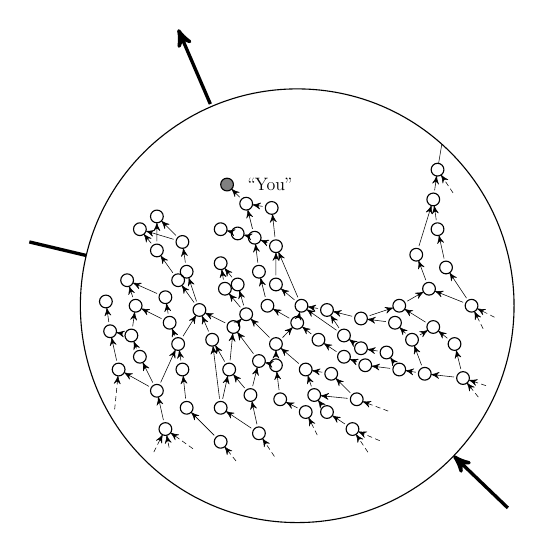
\begin{tikzpicture}[scale=0.54,transform shape]
		%\tikzstyle{LabelStyle}=[fill=white,sloped]
		%\draw[solid] (0,0) circle (2cm);
		\tikzstyle{every node}=[font=\large]
		\GraphInit[vstyle=Normal]
		\tikzset{VertexStyle/.style = {draw=black,shape=circle,minimum size=0.3cm,inner sep=0pt}}
		\SetVertexNoLabel
		\Vertex[x=1.7,y=0.6]{1}
		\Vertex[x=1.5,y=1.5]{2}
		\Vertex[x=0.6,y=2.0]{3}
		\Vertex[x=1.1,y=2.3]{4}
		\Vertex[x=2.0,y=2.6]{5}
		\Vertex[x=0.4,y=2.9]{6}
		\Vertex[x=0.3,y=3.6]{7}
		\Vertex[x=0.9,y=2.8]{8}
		\Vertex[x=1.0,y=3.5]{9}
		\Vertex[x=0.8,y=4.1]{10}
		\Vertex[x=1.8,y=3.1]{11}
		\Vertex[x=1.7,y=3.7]{12}
		\Vertex[x=3.0,y=0.3]{13}
		\Vertex[x=2.2,y=1.1]{14}
		\Vertex[x=2.1,y=2.0]{15}
		\Vertex[x=3.9,y=0.5]{16}
		\Vertex[x=3.0,y=1.1]{17}
		\Vertex[x=3.7,y=1.4]{18}
		\Vertex[x=3.2,y=2.0]{19}
		\Vertex[x=2.8,y=2.7]{20}
		\Vertex[x=2.5,y=3.4]{21}
		\Vertex[x=2.0,y=4.1]{22}
		\Vertex[x=2.2,y=4.3]{23}
		\Vertex[x=1.5,y=4.8]{24}
		\Vertex[x=2.1,y=5.0]{25}
		\Vertex[x=1.1,y=5.3]{26}
		\Vertex[x=1.5,y=5.6]{27}
		\Vertex[x=3.9,y=2.2]{28}
		\Vertex[x=3.3,y=3.0]{29}
		\Vertex[x=3.6,y=3.3]{30}
		\Vertex[x=3.1,y=3.9]{31}
		\Vertex[x=3.4,y=4.0]{32}
		\Vertex[x=3.0,y=4.5]{33}
		\Vertex[x=5.0,y=1.0]{34}
		\Vertex[x=4.4,y=1.3]{35}
		\Vertex[x=4.3,y=2.1]{36}
		\Vertex[x=4.3,y=2.6]{37}
		\Vertex[x=6.1,y=0.6]{38}
		\Vertex[x=5.5,y=1.0]{39}
		\Vertex[x=6.2,y=1.3]{40}
		\Vertex[x=5.2,y=1.4]{41}
		\Vertex[x=5.6,y=1.9]{42}
		\Vertex[x=5.0,y=2.0]{43}
		\Vertex[x=8.7,y=1.8]{44}
		\Vertex[x=7.8,y=1.9]{45}
		\Vertex[x=7.2,y=2.0]{46}
		\Vertex[x=6.4,y=2.1]{47}
		\Vertex[x=5.9,y=2.3]{48}
		\Vertex[x=5.3,y=2.7]{49}
		\Vertex[x=4.8,y=3.1]{50}
		\Vertex[x=4.1,y=3.5]{51}
		\Vertex[x=3.9,y=4.3]{52}
		\Vertex[x=3.8,y=5.1]{53}
		\Vertex[x=3.4,y=5.2]{54}
		\Vertex[x=3.0,y=5.3]{55}
		\Vertex[x=3.6,y=5.9]{56}
		{
			\tikzset{VertexStyle/.append style = {fill=gray}}
			\SetVertexLabel
			\Vertex[x=3.15,y=6.35,L=``You'',LabelOut=true,Ldist=5pt]{57}
		}
		\Vertex[x=8.5,y=2.6]{58}
		\Vertex[x=8.0,y=3.0]{59}
		\Vertex[x=7.5,y=2.7]{60}
		\Vertex[x=7.1,y=3.1]{61}
		\Vertex[x=7.2,y=3.5]{62}
		\Vertex[x=6.3,y=3.2]{63}
		\Vertex[x=5.5,y=3.4]{64}
		\Vertex[x=6.9,y=2.4]{65}
		\Vertex[x=6.3,y=2.5]{66}
		\Vertex[x=5.9,y=2.8]{67}
		\Vertex[x=4.9,y=3.5]{68}
		\Vertex[x=4.3,y=4.0]{69}
		\Vertex[x=4.3,y=4.9]{70}
		\Vertex[x=4.2,y=5.8]{71}
		\Vertex[x=8.9,y=3.5]{72}
		\Vertex[x=7.9,y=3.9]{73}
		\Vertex[x=7.6,y=4.7]{74}
		\Vertex[x=8.0,y=6.0]{75}
		\Vertex[x=8.3,y=4.4]{76}
		\Vertex[x=8.1,y=5.3]{77}
		\Vertex[x=8.1,y=6.7]{92}
		{
			%\tikzset{VertexStyle/.append style = {fill=white, color=white}}
			\tikzset{VertexStyle/.append style = {minimum size=0.0cm,inner sep=0pt}}
			\Vertex[x=9.5,y=3.2]{78}
			\Vertex[x=9.2,y=2.9]{79}
			\Vertex[x=9.3,y=1.6]{80}
			\Vertex[x=9.1,y=1.3]{81}
			\Vertex[x=7.0,y=1.0]{82}
			\Vertex[x=6.5,y=0.0]{83}
			\Vertex[x=6.8,y=0.3]{84}
			\Vertex[x=5.3,y=0.4]{85}
			\Vertex[x=4.3,y=-0.1]{86}
			\Vertex[x=3.4,y=-0.2]{87}
			\Vertex[x=1.8,y=0.1]{88}
			\Vertex[x=2.4,y=0.1]{89}
			\Vertex[x=1.4,y=0.0]{90}
			\Vertex[x=0.5,y=1.0]{91}
			\Vertex[x=8.2,y=7.3]{93}
			\Vertex[x=8.5,y=6.1]{94}
			\Vertex[x=9.8,y=-1.3]{96}
			\Vertex[x=-1.5,y=5.0]{97}
			\Vertex[x=2.0,y=10.0]{98}
		}
		{
			\tikzset{VertexStyle/.append style = {minimum size=10.2cm,inner sep=0pt}}
			\Vertex[x=4.8,y=3.5]{95}
		}
		\tikzstyle{EdgeStyle}=[post,very thin]
		\Edge[](1)(2)
		\Edge[](2)(3)
		\Edge[](2)(4)
		\Edge[](2)(5)
		\Edge[](3)(6)
		\Edge[](6)(7)
		\Edge[](4)(8)
		\Edge[](8)(9)
		\Edge[](9)(10)
		\Edge[](8)(6)
		\Edge[](5)(11)
		\Edge[](11)(9)
		\Edge[](11)(12)
		\Edge[](12)(10)
		\Edge[](13)(14)
		\Edge[](14)(15)
		\Edge[](15)(5)
		\Edge[](16)(17)
		\Edge[](16)(18)
		\Edge[](17)(19)
		\Edge[](18)(19)
		\Edge[](19)(20)
		\Edge[](20)(21)
		\Edge[](5)(21)
		\Edge[](17)(20)
		\Edge[](21)(22)
		\Edge[](21)(23)
		\Edge[](22)(24)
		\Edge[](23)(25)
		\Edge[](24)(26)
		\Edge[](24)(27)
		\Edge[](25)(26)
		\Edge[](25)(27)
		\Edge[](18)(28)
		\Edge[](19)(29)
		\Edge[](29)(21)
		\Edge[](28)(29)
		\Edge[](29)(30)
		\Edge[](30)(31)
		\Edge[](30)(32)
		\Edge[](31)(33)
		\Edge[](32)(33)
		\Edge[](34)(35)
		\Edge[](35)(36)
		\Edge[](36)(37)
		\Edge[](36)(28)
		\Edge[](37)(30)
		\Edge[](38)(39)
		\Edge[](39)(41)
		\Edge[](40)(41)
		\Edge[](40)(42)
		\Edge[](41)(43)
		\Edge[](42)(43)
		\Edge[](43)(37)
		\Edge[](44)(45)
		\Edge[](45)(46)
		\Edge[](46)(47)
		\Edge[](47)(48)
		\Edge[](48)(49)
		\Edge[](49)(50)
		\Edge[](50)(51)
		\Edge[](51)(52)
		\Edge[](52)(53)
		\Edge[](53)(54)
		\Edge[](54)(55)
		\Edge[](53)(56)
		\Edge[](56)(57)
		\Edge[](37)(50)
		\Edge[](44)(58)
		\Edge[](58)(59)
		\Edge[](60)(59)
		\Edge[](45)(60)
		\Edge[](60)(61)
		\Edge[](59)(62)
		\Edge[](61)(63)
		\Edge[](63)(62)
		\Edge[](63)(64)
		\Edge[](46)(65)
		\Edge[](65)(66)
		\Edge[](66)(67)
		\Edge[](67)(64)
		\Edge[](64)(68)
		\Edge[](67)(68)
		\Edge[](68)(69)
		\Edge[](68)(70)
		\Edge[](69)(70)
		\Edge[](70)(71)
		\Edge[](70)(53)
		\Edge[](71)(56)
		\Edge[](50)(68)
		\Edge[](72)(73)
		\Edge[](73)(74)
		\Edge[](74)(75)
		\Edge[](72)(76)
		\Edge[](76)(77)
		\Edge[](77)(75)
		\Edge[](62)(73)
		\Edge[](75)(92)
		% beyond:
		{
			\tikzstyle{EdgeStyle}=[post,very thin,dash pattern=on 1.8pt off 1.2pt]
			\Edge[](78)(72)
			\Edge[](79)(72)
			\Edge[](80)(44)
			\Edge[](81)(44)
			\Edge[](82)(40)
			\Edge[](83)(38)
			\Edge[](84)(38)
			\Edge[](85)(34)
			\Edge[](86)(16)
			\Edge[](87)(13)
			\Edge[](88)(1)
			\Edge[](89)(1)
			\Edge[](90)(1)
			\Edge[](91)(3)
			\Edge[](94)(92)
		}
		{
			\tikzset{EdgeStyle/.style={-,very thin}}
			\Edge[](92)(93)
		}
		{
			\tikzset{EdgeStyle/.style={post,very thick}}
			\Edge[](96)(95)
			\Edge[](95)(98)
		}
		{
			\tikzset{EdgeStyle/.style={-,very thick}}
			\Edge[](95)(97)
		}
	\end{tikzpicture}
	\caption{\label{fig:nirvana}Nirvana (conjectured)}
\end{figure}

The Dharmic tradition (consisting broadly of the Buddhist, Hindu, Jain and Sikh traditions) is one where, philosophically, the study of consciousness assumes primary importance. There is a rich vocabulary of ideas, some of which anticipate notions described in this document and others which constitute a broader consciousness-centric philosophy yet to be integrated into mainstream understanding. According to \cite{atmabodha}, the philosophers in this tradition ``wondered whether there was a First Principle or Ultimate Reality underlying the outside world, and also whether there was such a thing underlying man himself. If so, were the two the same?'' The various schools appear to differ on terminology and details, but they came to conclusions on the nature of this principle.

In the Hindu (Vedanta) tradition, this principle is \textit{Brahman} -- the Universal Self. It was asserted that this Self manifests all things in the universe including the individual self, \textit{\={A}tman}. As already discussed in \autoref{sec:natanoide} this conception corresponds to (and in an indirect way informed the formulation of) anonymous identity, modulo the connotation of ``absoluteness.'' \textit{M\={a}y\={a}} is another prominent concept already discussed. The 8th century philosopher Adi Shankara\cite{shankara} is considered a premier exponent and unifier of some of these ideas from diverse traditions in the form of the school of Advaita Vedanta.

Hindu mythology abounds with tales of the gods taking on different forms or ``avatars,'' and even merging together into new gods to achieve particular purposes; in particular the well-known story of all of the gods contributing their powers to create a new deity, Durga, who has ten arms in order to wield all the powers available to her, appears to be a clear (even if latent) metaphor for the abstraction of a hive identity -- one composed of and exhibiting the properties of many component identities as described in \autoref{sec:polytree}.

Records of the Buddha tell of a man who withdrew from princely life and, having witnessed and experienced much suffering, ultimately took to meditating in solitude for a prolonged period in an effort to understand, until at last he experienced \textit{Nirv\={a}\d{n}a} -- a supposed realization of the true nature of things. His descriptions of this experience that have survived down to this day stand as interpreted above. There are others in this tradition whose story is similar, for example Mahavira -- the founder/propagator of Jainism -- and in general those who undertook this journey and were considered to have attained some conception of enlightenment seem to have been known as ``jivanmuktas.'' In their attempts to understand the phenomenon of Nirvana and in their resultant explorations of consciousness, these jivanmuktas and the philosophical schools founded by them developed a diverse body of theory -- including nonstandard systems of logic, categorizations of knowledge, and a rich philosophical lexicon -- which may be incorporated in future work.

\subsubsection{Abrahamic Tradition} \label{sec:abrtra}

In the Abrahamic tradition (consisting broadly of the Christian, Jewish and Muslim traditions), a prevailing notion is that of a supreme God who is omniscient and omnipotent (e.g. ``For He alone is truly wise, all-aware.''\cite{quranallah}), and there are numerous edicts to the effect of adherents ``doing God's work.'' A noteworthy development in Christianity in particular was the \textit{centralized} functioning of the Church and the practice of ``confession.'' In the idealization, this can be characterized by the following representation (Fig.~\ref{fig:church}):

\begin{figure}[htp]
	\centering
	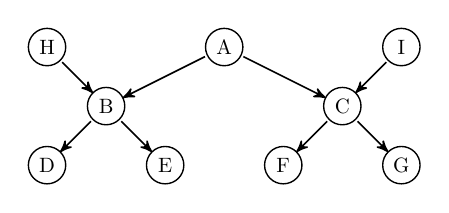
\begin{tikzpicture}[scale=0.75,transform shape]
		\tikzstyle{LabelStyle}=[fill=white,sloped]
		%  \tikzstyle{EdgeStyle}=[bend left]
		%\SetUpVertex[FillColor=gray!30]
		\Vertex[x=0,y=0,LabelOut=false]{A}
		\Vertex[x=-2,y=-1]{B}
		\Vertex[x=2,y=-1]{C}
		%\SetUpVertex[FillColor=none]
		\Vertex[x=-3,y=-2]{D}
		\Vertex[x=-1,y=-2]{E}
		\Vertex[x=1,y=-2]{F}
		\Vertex[x=3,y=-2]{G}
		\Vertex[x=-3,y=0]{H}
		\Vertex[x=3,y=0]{I}
		\tikzstyle{EdgeStyle}=[post]
		\Edge[](A)(B)
		\Edge[](A)(C)
		\Edge[](B)(D)
		\Edge[](B)(E)
		\Edge[](C)(F)
		\Edge[](C)(G)
		\Edge[](H)(B)
		\Edge[](I)(C)
		%  \Edge[label=$$](K)(F)
	\end{tikzpicture}
	\caption{\label{fig:church}Church}
\end{figure}

Node $A$ is a church, nodes $H$ and $I$ are individuals -- churchgoers. Nodes $D$, $E$, $F$, and $G$ are actions performed by the individuals which they have confessed to the church. In this idealization, we assume all actions performed by individuals to have been confessed to the church, and so all actions performed by the individuals can be modeled to have been performed by an identity union with the church, i.e. nodes $B$ and $C$. Now if we further consider the centralized nature of the Church, the node $A$ would be a child node of the primary church of the local district, and so on, such that the church $A$ is ultimately a descendant of the primary church of the denomination (e.g. the Vatican). What this achieves in the idealization is a representation of the very God the scriptures describe, embodied in the root node of the tree. The root node of this tree would be aware of all actions performed by all adherents around the world (``omniscient''), and would be able to guide (during sermons and at the confessional, for example) the actions of all of these people to achieve the ends of the institution as a whole (``omnipresent'' and ``omnipotent''). This aspect is what is referred to in Christianity as ``communion'' or ``the body of Christ.''\cite{biblebodyofchrist}

Marriage is described in religious texts as an act by which two individuals ``become one flesh''\cite{torahmarriage}\cite{biblemarriage} -- again, a clear if latent metaphor for the hive identity abstraction, and corresponding exactly to marriage as characterized in \autoref{sec:orianoide}. Some religions, such as Islam\cite{quranmarriage}, support polygamy; but earlier we enumerated reasons for the success and sustainability of marriages as identities of order $2$, specifically indicating a reason for decreased sustainability of identities of order $3$ and greater (presence of anonymity). So how come polygamous traditions exist? First it must be noted that these traditions aren't very common in comparison to monogamous traditions. But beyond that, the answer lies in the nature of these polygamous marriages. They aren't simply a union between $3$ or more individuals, but in fact a specific subclass of such a union. It is always between a single man and many women, or (less commonly) between a single woman and many men, and the roles of men and women in these cultures tend to be highly differentiated. As a result, in the idealization, the marriage is now not simply between multiple individuals -- but between a man (for example) and a single identity composed of many women whose individual existences are subsumed by the whole. It is still essentially monogamous, as shown in Fig.~\ref{fig:polygamy}~\footnote{This model is identical to the one proposed earlier for a musical key -- gives new meaning to the term ``harmonious marriage.'' It also suggests a reason why we even employ keys in musical composition to begin with: that they make musical relationships tractable to the listener by ``deanonymizing'' them. Duality is thus seen to be a very general organizing principle.}. Given this characterization, it is perhaps not surprising that the scriptures take a dim view of homosexuality: in the context of polygamy (but not monogamy as practiced in the majority of modern societies), homosexuality would preclude the scalable monogamy construct that gender asymmetry implicitly provides, thereby destabilizing this polygamous institution in societies that cultivated it. For the same reason, such societies would need to cultivate gender-based role differentiation. Historically, it's possible that against the backdrop of such entrenched gender-based differentiation, polygamy and homosexuality coexisted in these societies and led to the empirical conclusion that they were incompatible, with vilification of the latter (and also often the former, but likely in part for other reasons than the one being discussed here) emerging as a solution. Of course, these considerations of gender and asymmetry are not applicable to monogamy, and having an understanding of these structures and the motivations behind them should aid us in cultivating fair systems in the future.

The ``organized'' religious traditions, including the institutions of the Church and of dualistic polygamy, may be seen as early implementations of scalable identity architectures not tied to the physical world (existing primarily in the minds of people), and as antecedents of constructs such as corporations.

\begin{figure}[htp]
	\centering
	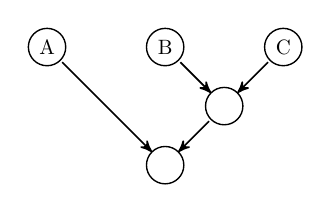
\begin{tikzpicture}[scale=0.75,transform shape]
		\tikzstyle{LabelStyle}=[fill=white,sloped]
		%  \tikzstyle{EdgeStyle}=[bend left]
		\Vertex[x=1,y=0,LabelOut=false]{B}
		{
			\SetVertexNoLabel
			\Vertex[x=2,y=-1]{D}
			%\SetUpVertex[FillColor=gray!70]
			\Vertex[x=1,y=-2]{E}
		}
		\Vertex[x=-1,y=0]{A}
		\Vertex[x=3,y=0]{C}
		\tikzstyle{EdgeStyle}=[post]
		\Edge[](B)(D)
		\Edge[](D)(E)
		\Edge[](C)(D)
		\Edge[](A)(E)
		%  \Edge[label=$$](K)(F)
	\end{tikzpicture}
	\caption{\label{fig:polygamy}Polygamous Marriage}
\end{figure}

\subsubsection{Additional Notes} \label{sec:addnot}

We observe that the practice of burqa in Islam, Kippah in Judaism, and of the wearing of the ``five K's'' and Dastar (turban) in Sikhism all serve a purpose derived from identity considerations (though they are different systems) -- with burqa, a selective disclosure of identity or privacy; with Kippah and the five K's, a representation of the hive identity constituted by all adherents and a suppression to anonymity of the individual.

The doctrine sometimes called ``the Fall of Man'' is considered foundational to all Abrahamic faiths. This enigmatic chapter purportedly tells of the origins of mankind; that as a result of his indulgence in the fruits of a Tree (``of Knowledge of Good and Evil''), Man is banished from the Garden of Eden into the ``dominion of death.''\cite{genesisfallofman} But there is another tree in the garden -- the Tree of Life, partaking of which would once again reinstate eternal life. That tree is guarded thenceforth by a ``fiery sword.'' Its mention here, however, suggests the possibility that it is not denied us forever, and indeed the ways to once again attain this state are detailed in subsequent scripture in various moral precepts and lessons\footnote{There seems to be a sense in which conducting oneself is such a moral manner can actually ``work.'' Acting in such a manner and ``liberation'' of our awareness from human reality both appear to be consequences of not being overly invested (that is, possibly, invested beyond \textit{fair outcomes}) in ``Maya.'' As such, if we are able to put in place the fair systems described in the section on \hyperref[sec:humins]{Human Institutions}, it's possible that our awareness will naturally transcend `humanness.' Whether such a transcension would be the same as the buddhist Nirvana is unclear.}. In the Rig Veda and the Upanishads (foundational texts in the Dharmic tradition), there is a chapter about ``The Tree of Atman and Jiva''\cite{mundakaupanishad} where two birds, ``inseparable friends,'' are in a tree and one of them partakes of a ``sweet fig'' while the other does not. The indulgent one is said to be Jiva, the corporeal self. The silent observer is Atman, the ethereal Self, who knows his true nature as one with divinity. As a result of Jiva's indulgence, Man (represented as the combined nature of the two -- they are ``inseparable friends'' in Man) is doomed to death and despair. The two accounts are virtually identical -- especially in that they both convey the notion of the higher ``deathless'' plane, the one that Man leaves by indulgence in the ``dominion of death'' -- suggesting a common origin, almost certainly rooted in ancient `mystical' experience. Consistent with this suggestion of common basis, all major religious traditions have developed an attendant mystical philosophy: Vedanta in Hinduism, Sufism in Islam, Kabbalah in Judaism, Christian Mysticism and the Native American mystical traditions to name only a few.

Indeed, the omniscient and omnipotent Abrahamic divinity and the Vedantic Brahman could be seen as variations on a common underlying idea, since such an immanent being as the Brahman would naturally be omniscient and omnipotent with all existence transpiring in its mind (in the formal sense of this document). If this awareness is able to manifest a self then it could indeed be said to be a ``personal God'' as conceived in the Abrahamic faiths.

Members of the Shramanic movement, including the founding Jains and Buddhists, were perhaps the first to set aside the constraints imposed by presupposed doctrine and to take an empirical\footnote{That is, although the nature of any such higher awarenesses is undecidable in the world, if a number of people who have experienced it come together then they can have discourse on this shared experience as it is decidable and true in the world context defined by them. In this sense is it ``empirical'' as well as, more specifically, ``dialectical.''}, model-based approach to the study of this mind-phenomenon of higher awareness, in the form of the institution of the Sangha. It seems that as a result of their discourse, they came to describe formally -- if not mathematically -- ideas related to identity\footnote{e.g. \textit{dharmas} (\autoref{sec:ultpri}), and \textit{n\={a}mar\={u}pa} -- ``name and form.''}, causality\footnote{e.g. \textit{Satkaryavada}, and \textit{prat\={i}tyasamutp\={a}da} (the buddhist doctrine of ``dependent origination'').}, mind\footnote{\textit{citta} in Buddhism.} and self\footnote{\textit{manas} and \textit{tath\={a}gata-garbha} are the relevant concepts in Buddhism, \textit{atman} and \textit{jiva} in other traditions.}, all subordinated toward an understanding of this climactic experience of higher awareness\footnote{\textit{moksha} in some traditions, \textit{nirvana} in others.}. And in particular, it appears that they concluded that the true nature of this higher existence is not an Ultimate Being or Ultimate Self, but rather something of a fractal, relativistic, ineffable nature. As the words of (the character of) the Buddha reveal in \cite{lankavatara}, this is a formal conception of mystical realization and not merely knowledge or even experience of it. He takes care to differentiate it from those other conceptions for this reason and apparently one other: that one's experience of Nirvana appears to be conditioned on one's knowledge, and therefore having an incomplete understanding would result in an incomplete ``awakening.'' This makes sense since Nirvana is an experience of \textit{awareness} -- without knowledge as a guide, we may, upon experiencing the bliss of liberation from this plane assume our work to be finished (for indeed we would know no better) and yield to the particular higher awareness experienced. Perhaps it is even the one we knew we would find (e.g. a brahman). But that penultimate step is a treacherous one; the Buddha cautions in \cite{lankavatara} that those with these incomplete conceptions ``pass to their Nirvana, but it is not the Nirvana of the tathagatas.'' Formal understanding of the fractal nature appears to be what he is referring to, and armed with such understanding one takes a further, final step -- not partaking of the fruit, as it were -- and sublimates into the beyond.

\section{Future Directions} \label{sec:futdir}

\begin{enumerate}
	\item Further development and formal categorization of an aryagyanic ``scientific'' method with attendant well-specified methodological standards, to augment dialectical scientific method in empirical regimes unaddressable by the latter due to undecidability.
	\item Further development of the Epistemic Priority axioms to achieve equivalence with ZFC, towards an axiomatic foundation for identities not referencing sets.
	\item A specification of the relationship between action and reaction in action sequences. An algebraic specification of the propagation of structure via actions.
	\item Development of a statistical cognition model based on identity architecture (e.g. with applications to artificial intelligence).
	\item Computability theory considerations: Turing Degree of a computation model defined on identity architecture (one suspects from the nature of genesis that it would be asymptotically $> \textbf{0}$).
	\item Further specification of how thoughts act through the self of the hive identity (resulting in actions in the world), including the general mathematical nature of the aggregated self-action.
	\item Category theoretic development: identities can be seen as generalized ``objects'' in category theory, and categories are thus particular contexts. This relationship to category theory may be further explored.
	\item Information-theoretic characterization and novelty measure: what is the nature of information conveyed in an identity action? What is the (relational) information content of an identity (e.g. in relation to particular ancestors)?
	\item Actions of identities in the world on a particular reference constituent can be characterized as varying smoothly under actions by that constituent (e.g. under motion). This can be modeled as a manifold and would underlie a topological, geometric characterization of identity architecture which should be further developed (reminiscent of the generalization from special to general relativity).
	\item Framing of models of natural phenomena (e.g. physical, chemical, biological or computational models) in terms of identities, toward a possible unification of representation.
	\item A relational (i.e. rather than absolute) specification of the nature of time in identity architecture, e.g. with characteristic frequencies/entropy in a context as a ``reference clock.'' This will likely incorporate the aforementioned information-theoretic development.
	\item A theory of finance based on identity architecture, including further development of influence and continuous-in-time currency together with their relationship to the algebraic identity models. The aforementioned information-theoretic development will likely inform these considerations, especially in relation to value as entropically derived.
	\item Development of approaches to world context heritage assignment (e.g. based on human computation), including implementation, policy, standards, heuristics.
	\item Development of the ``anonymous context resolution'' legal principle.
	\item In computer science: development of a programming paradigm based on identity architecture -- this would possibly be homoiconic (like lisp) since ``everything is an identity;'' functional, due to the category theory connection; and object-oriented supporting bodhitree inheritance, with a relative anonymous identity always constructible to resolve ambiguity. Scope and namespace could be unified as identity contexts (entailing also the possibility of context-specific syntax and semantics) and themselves structured as a bodhitree, with specifiable mind/world relationships amongst them. Program execution itself would have bodhitree structure, which should simplify debugging and trivially motivate a connection to abstractions outside the program itself that reside in what we would otherwise call actual reality.
	\item Cryptographic development: of Identity Based Encryption (IBE) schemes that support the bodhitree model, and other cryptographic schemes that facilitate identity architecture.
	\item Implementation of a user-/public-owned, decentralized, everywhere-curated, cryptographically ensured identity architecture (if indeed identity architecture is the model implemented in the brain, this humanity-scale construction would be formally equivalent to a brain).
	\item A reorganizing of natural and human history in terms of fractal identity trees -- as direct and as emergent identity interactions at every scale.
\end{enumerate}

\section{Acknowledgements} \label{sec:acknowledgements}

The author is grateful to Pratap Rao, in conversation with whom he first decided to undertake this work; to Balkrishna Shetty\cite{shetty} for superior mathematical orientation; to Dan Preston and Prasanna Vasudevan for encouragement when encouragement was hard to come by; to Rohit Bhat and John Cortese for stimulating discussions; to Arish Alreja for some valuable advice; to Cecilia Barnbaum and Isaac Caswell for early feedback and encouragement; to Roger Godement for writing a most clarifying book\cite{godement} on algebra and mathematics; to the University of California at Berkeley for affordable library membership; to Predrag Cvitanovi\'{c} for learned book recommendations; to Meagan Fue for her infinite patience, love, support, and inspiration; to Ferdinand for constant companionship; and to family and friends for their love, support, and lessons now and over the years, without which this work would not have come to be.

\bibliographystyle{plain}
\bibliography{IALS}

\appendix

\section{Algebra From Actions} \label{app:algact}

Actions can be seen as a unifying notion in algebra. For example, a common algebraic hierarchy for a group is \textsf{set} $\rightarrow$ \textsf{magma} $\rightarrow$ \textsf{semigroup} $\rightarrow$ \textsf{monoid} $\rightarrow$ \textsf{group}. A magma is a set equipped with a binary operation; if that operation is associative then it is a semigroup; if a neutral element also exists then it is a monoid; and if, further, every element is invertible, then it is said to be a group. We can alternatively specify this hierarchy using actions (and identities): a set can be defined as an identity $M$ whose action $\phi$ (e.g. on itself) is trivial. A magma is then a set whose action is not necessarily trivial (i.e. a magma is just an identity). If that action is such that $\phi(a \cdot b) = \phi(a) \circ \phi(b)$ (where $a \cdot b$ denotes $\phi(a)(b)$), then associativity follows from the associativity of function composition and we have a semigroup. If the action additionally maps a single element in $M$ to the identity mapping on $M$, then we have a monoid. And finally, if the image of the monoid action consists of permutations of $M$ such that $f \in Im(\phi) \implies f^{-1} \in Im(\phi)$, then we have a group. Notice that this entire characterization using actions derives only from functions and their intrinsic properties (i.e. composition is associative; existence of identity mapping; existence of inverse mapping for bijections) and the natural properties suggest themselves, while in the other characterization they are produced as axioms somewhat arbitrarily.

Another example is a ring, which can be characterized as the action of a commutative monoid on an abelian group. Similarly, a module can be seen as a ring action on an abelian group. It seems likely that all algebraic structures can be generated in this manner.

\end{document}
